% Options for packages loaded elsewhere
\PassOptionsToPackage{unicode}{hyperref}
\PassOptionsToPackage{hyphens}{url}
\documentclass[
]{article}
\usepackage{xcolor}
\usepackage{amsmath,amssymb}
\setcounter{secnumdepth}{-\maxdimen} % remove section numbering
\usepackage{iftex}
\ifPDFTeX
  \usepackage[T1]{fontenc}
  \usepackage[utf8]{inputenc}
  \usepackage{textcomp} % provide euro and other symbols
\else % if luatex or xetex
  \usepackage{unicode-math} % this also loads fontspec
  \defaultfontfeatures{Scale=MatchLowercase}
  \defaultfontfeatures[\rmfamily]{Ligatures=TeX,Scale=1}
\fi
\usepackage{lmodern}
\ifPDFTeX\else
  % xetex/luatex font selection
\fi
% Use upquote if available, for straight quotes in verbatim environments
\IfFileExists{upquote.sty}{\usepackage{upquote}}{}
\IfFileExists{microtype.sty}{% use microtype if available
  \usepackage[]{microtype}
  \UseMicrotypeSet[protrusion]{basicmath} % disable protrusion for tt fonts
}{}
\makeatletter
\@ifundefined{KOMAClassName}{% if non-KOMA class
  \IfFileExists{parskip.sty}{%
    \usepackage{parskip}
  }{% else
    \setlength{\parindent}{0pt}
    \setlength{\parskip}{6pt plus 2pt minus 1pt}}
}{% if KOMA class
  \KOMAoptions{parskip=half}}
\makeatother
\usepackage{longtable,booktabs,array}
\usepackage{caption}
\captionsetup[table]{skip=6pt}
\newcounter{none} % for unnumbered tables
\usepackage{calc} % for calculating minipage widths
% Correct order of tables after \paragraph or \subparagraph
\usepackage{etoolbox}
\makeatletter
\patchcmd\longtable{\par}{\if@noskipsec\mbox{}\fi\par}{}{}
\makeatother
% Allow footnotes in longtable head/foot
\IfFileExists{footnotehyper.sty}{\usepackage{footnotehyper}}{\usepackage{footnote}}
\makesavenoteenv{longtable}
\usepackage{graphicx}
\makeatletter
\newsavebox\pandoc@box
\newcommand*\pandocbounded[1]{% scales image to fit in text height/width
  \sbox\pandoc@box{#1}%
  \Gscale@div\@tempa{\textheight}{\dimexpr\ht\pandoc@box+\dp\pandoc@box\relax}%
  \Gscale@div\@tempb{\linewidth}{\wd\pandoc@box}%
  \ifdim\@tempb\p@<\@tempa\p@\let\@tempa\@tempb\fi% select the smaller of both
  \ifdim\@tempa\p@<\p@\scalebox{\@tempa}{\usebox\pandoc@box}%
  \else\usebox{\pandoc@box}%
  \fi%
}
% Set default figure placement to htbp
\def\fps@figure{htbp}
\makeatother
\setlength{\emergencystretch}{3em} % prevent overfull lines
\providecommand{\tightlist}{%
  \setlength{\itemsep}{0pt}\setlength{\parskip}{0pt}}
\usepackage{bookmark}
\IfFileExists{xurl.sty}{\usepackage{xurl}}{} % add URL line breaks if available
\urlstyle{same}
% fallback for those not using the hyperref driver hyperxmp:
\makeatletter
\@ifundefined{xmpquote}{\newcommand{\xmpquote}[1]{#1}}{}
\makeatother
\hypersetup{
  hidelinks,
  pdfcreator={LaTeX via pandoc}}

\author{}
\date{}

\begin{document}

{
\setcounter{tocdepth}{3}
\tableofcontents
}
\section{The Failure-Prediction Monitor Does Not
Transfer:}\label{the-failure-prediction-monitor-does-not-transfer}

\section{A Cross-Context Empirical Investigation (RL, MARL,
LLM)}\label{a-cross-context-empirical-investigation-rl-marl-llm}

\subsection{Y5 Master Synthesis Paper
(v1.3)}\label{y5-master-synthesis-paper-v1.3}

\textbf{v1.3 additions} (addresses 6 v1.2 reviewer items, all P3
very-minor): - Pre-Reg P3 adds explicit GPU reservation (R1.5):
\textasciitilde50 GPU-hours, 2026-08-01 to 2026-08-15 window - Section
5.3.2 n=5 Hedges g row provenance note (R1.6): marks d = -0.250 as
post-hoc - Section 8.5 Pattern D cross-reference (R2.5): links to
Pre-Reg PROP3-HYBRID.md - Bibliography adds 7 references (R2.6 +
extended): Shimodaira 2000 / Cover \& Thomas 1991 / Valiant 1984 /
Haussler 1990 / Hanley-McNeil 1982 / Holm 1979 / Hedges 1981 - Section
7.6.6 formal monotonicity lemma (R3.5): partial order on \{R1,R2,R3,R4\}
+ 16-cell framework-update table + proof - Section 7.6.3 cost-weighted
observation (R3.6): per-Refutation GPU-hour budget + Archimedes Project
test priority order

\textbf{v1.2 additions} (addresses 10 reviewer items): - Section 5.3.2
-- Extended meta-analysis (Bonferroni-Holm + Hedges g + forest plot) -
Section 7.5.5 -- First-principles motivation (PAC-learning +
distribution-shift + info-theory) - Section 7.6.1 footnote --
Hanley-McNeil bound for Definition 6 - Section 7.6.1 paragraph --
Decomposition uniqueness justification - Section 7.6.2 footnote --
Required-n assumed effect size - Section 7.6.3 paragraph -- Logical
disjunction of R1-R4 - Section 7.6.3 footnote -- R4 compute-cost
estimate (7B / 70B) - Section 7.6.6 -- Monotonicity of refutation
observation - Section 8.5 -- Concrete deployment patterns (4 patterns) -
Section 9.6 -- Limitations of the formal framework itself

\textbf{v1.1 additions} (addresses 2 P0 reviewer items): - Section 5.3.1
-- Cross-task combined-p meta-analysis (Fisher, Stouffer, Bonferroni) -
Section 7.6.2 -- Assumption A1 explicitly named (positive mutual
information between auxiliary signal and policy value function) -
Section 7.6 framework diagram (3 Convergence + 4 Refutations + 4
Propositions) embedded as Figure 1

\begin{quote}
\textbf{Authors:} Liu Zewen + Codex (Archimedes Project, AGI-2026-001)\\
\textbf{Date:} 2026-07-31 (Y4 v0.6.1 verdict:
STOP-PAPER-REFUTED-REVERSE)\\
\textbf{Status:} v0.8 draft. Integrates Y1 single-agent RL (validated),
Y3 multi-agent MARL (5/6 pathways REFUTED + 1 positive v8 dlr\_only), Y4
H10 LLM self-monitoring (4 pre-registered sample-size replications,
REFUTED consistent negative direction across 2 task families).\\
\textbf{Code:}
\texttt{projects/project\_g\_llm\_self\_monitoring/code/}\\
\textbf{Data:} \texttt{experiments\_log/\_h10\_*\_bootstrap.json},
\texttt{\_v8\_sanity\_4seed.json}, \texttt{\_h10\_n20\_summary.json}\\
\textbf{Pre-registrations:}
\texttt{experiments\_log/2026-07-28-PRE-REGISTERED-H10.md},
\texttt{2026-07-31-PRE-REGISTRATION-AMENDMENT-1.md}, addendum\\
\textbf{Companion papers:} Y1 (\texttt{papers/y1\_paper\_draft.md}), Y3
(\texttt{papers/monitor\_signal\_vs\_dlr\_6pathway.md}), Y4
(\texttt{papers/project\_g\_v0\_5\_h10\_paper.md})\\
\textbf{Target venue:} Major LLM/ML venue (e.g., COLM 2026, NeurIPS 2026
workshop, ICML workshop)
\end{quote}

\subsection{Abstract}\label{abstract}

We investigate whether the \textbf{failure-prediction Monitor} -- a
small auxiliary classifier trained on a frozen reference policy's
trajectories that predicts trajectory-level failure -- transfers as a
training signal across three fundamentally different agent contexts:
\textbf{single-agent reinforcement learning (RL)}, \textbf{cooperative
multi-agent RL (MARL)}, and \textbf{LLM self-monitoring}. Across three
independent pre-registered investigations totaling several thousand
training runs, we find a \textbf{consistent pattern}: the Monitor is a
\textbf{verified context-specific signal} that produces a strong effect
in the exact regime where it was verified (single-agent RL) but does NOT
transfer beyond that regime. Specifically:

\begin{itemize}
\tightlist
\item
  **H1 single-agent RL (Y1, validated, 39 seeds across extensions):
  frozen-decoupled Monitor as reward shaping gives +39.5 mean
  improvement on LunarLander-v3 (n=15 seeds, t=6.76, p\textless0.001).
  Verified, reproducible across multiple sample sizes. See Y1 paper for
  the canonical 15-seed result.
\item
  \textbf{H5 multi-agent MARL (Y3, 6-pathway systematic investigation,
  5-100 seeds per arm): of 6 architectures that incorporate the Monitor,
  }5 are REFUTED at p\textless0.05** and 1 (v8 dlr\_only) has only a
  small positive effect (+0.1447 at n=30, shrinking to +0.0617 at n=100,
  95\% CI {[}+0.0084, +0.1149{]}, Bonferroni-corrected p=0.0433).
  Critically, \textbf{that single positive result is NOT from the
  Monitor but from hand-crafted DLR predicates} that operate on the
  critic, not the Monitor.
\item
  \textbf{H10 LLM self-monitoring (Y4, 4 pre-registered sample-size
  replications): the Frozen-vs-Joint Monitor contrast is at chance level
  across all 4 sample sizes / 2 task families. At n=100 simple
  arithmetic, Cohen's d = +0.030 (F-J = +0.015, 95\% CI {[}-0.087,
  +0.117{]}, n=98 valid). At n=20 GSM8K 200-token chain-of-thought,
  Cohen's d = -0.120 (F-J = -0.053, 95\% CI {[}-0.237, +0.158{]},
  p=0.714, n=19 valid). }Pre-registered kill switch verdict:
  \texttt{STOP-PAPER-REFUTED-REVERSE}** -- H10 REFUTED with consistent
  negative direction (Joint \textgreater{} Frozen) across both task
  families.
\end{itemize}

The pattern is robust across \textbf{5 of 6 multi-agent Monitor-using
pathways REFUTED, 4 of 4 LLM H10 sample sizes REFUTED, 0 of 1
single-agent pathway REFUTED} (Y1 holds). The Monitor signal does not
generalize beyond single-agent RL. We propose a unified framework -- the
\textbf{Monitor as a context-specific signal} -- that predicts when the
Monitor will and will not transfer. The framework rests on three
convergence conditions: (1) the policy distribution matches between
Monitor training and Monitor consumption; (2) the failure mode of
interest is observable in the Monitor's features; (3) the
signal-to-noise ratio of the Monitor's prediction is high enough to be a
useful training signal. The Monitor fails to transfer outside its
verified regime because at least one of these conditions breaks.

\textbf{Practical implication for the field}: the Monitor's verified
shipping use remains \textbf{verification} (DLR predicates in critic,
runtime guardrails), NOT as a training signal in untested
configurations. We recommend that researchers pre-register the Monitor's
intended context of use and validate empirically before deploying as a
training-time regularizer.

\subsection{1. Introduction}\label{introduction}

The failure-prediction Monitor is one of the most robust findings in the
Archimedes Project, a multi-year investigation of auxiliary-agent
training signal design. In the Y1 paper (validated LunarLander-v3 PPO
study), a small classifier trained on a frozen Stage-1 policy's
trajectories can predict trajectory-level failure with AUROC 0.796 vs a
joint-trained Monitor's 0.072. When this prediction is used as a reward
penalty (-Monitor(failure\_prob) * 0.5), the policy improves by +39.5
mean reward (n=15 seeds, t=6.76, p\textless0.001).

Three architectural features of the Y1 Monitor are critical to its
success:

\begin{enumerate}
\def\labelenumi{\arabic{enumi}.}
\tightlist
\item
  \textbf{Frozen}: the Monitor is trained on a frozen reference policy,
  not jointly with the agent. Joint training produces a Monitor that
  learns to predict self-fulfilling outcomes, not the true failure mode.
\item
  \textbf{Decoupled}: there is one Monitor per agent, not one shared
  Monitor. A shared Monitor across agents would have ambiguous credit
  assignment.
\item
  \textbf{Reward penalty} (not classification loss): the Monitor's
  prediction is used as a reward signal, not as the direct
  classification objective. The reward shaping formulation lets the
  policy learn to AVOID failure modes predicted by the Monitor, even if
  those predictions are imperfect.
\end{enumerate}

The Monitor's success in single-agent RL prompts the natural and
important question: \textbf{does the Monitor transfer to other
contexts}? Specifically:

\begin{itemize}
\tightlist
\item
  Does it transfer to cooperative multi-agent RL where the joint Monitor
  failure mode is more acute (the policy is non-stationary across
  training)?
\item
  Does it transfer to LLM self-monitoring where the `policy' is a
  fine-tuned language model rather than a tabula-rasa PPO policy?
\item
  Does it transfer across sample sizes (n=5 -\textgreater{} n=20
  -\textgreater{} n=100 -\textgreater{} n=200)?
\item
  Does it transfer across task families (simple arithmetic vs
  chain-of-thought reasoning vs continuous-control vs multi-agent credit
  assignment)?
\end{itemize}

We designed three independent pre-registered investigations to answer
these questions. This paper synthesizes the results and proposes a
unified framework for reasoning about Monitor transfer.

\subsubsection{1.1 The three investigations at a
glance}\label{the-three-investigations-at-a-glance}

{\def\LTcaptype{none} % do not increment counter
\begin{longtable}[]{@{}
  >{\raggedright\arraybackslash}p{(\linewidth - 10\tabcolsep) * \real{0.1667}}
  >{\raggedright\arraybackslash}p{(\linewidth - 10\tabcolsep) * \real{0.1667}}
  >{\raggedright\arraybackslash}p{(\linewidth - 10\tabcolsep) * \real{0.1667}}
  >{\raggedright\arraybackslash}p{(\linewidth - 10\tabcolsep) * \real{0.1667}}
  >{\raggedright\arraybackslash}p{(\linewidth - 10\tabcolsep) * \real{0.1667}}
  >{\raggedright\arraybackslash}p{(\linewidth - 10\tabcolsep) * \real{0.1667}}@{}}
\toprule\noalign{}
\begin{minipage}[b]{\linewidth}\raggedright
Investigation
\end{minipage} & \begin{minipage}[b]{\linewidth}\raggedright
Context
\end{minipage} & \begin{minipage}[b]{\linewidth}\raggedright
Hypothesis
\end{minipage} & \begin{minipage}[b]{\linewidth}\raggedright
N
\end{minipage} & \begin{minipage}[b]{\linewidth}\raggedright
Verdict
\end{minipage} & \begin{minipage}[b]{\linewidth}\raggedright
Key statistic
\end{minipage} \\
\midrule\noalign{}
\endhead
\bottomrule\noalign{}
\endlastfoot
\textbf{Y1 single-agent RL} & LunarLander-v3 PPO & H1.3 frozen-decoupled
Monitor helps & 15 seeds (canonical), 39 across extensions &
\textbf{VALIDATED} & +39.5 mean, t=6.76, p\textless0.001 \\
\textbf{Y3 multi-agent MARL} & PettingZoo Simple Spread v3, MADDPG v2 &
H5 decoupled Monitor helps MA & 5-100 seeds/arm x 6 architectures &
\textbf{REFUTED (5/6)}; v8 dlr\_only +0.1447 -\textgreater{} +0.06 & v8
n=30 p\textless0.005; v8 n=100 p\_bonf=0.043 \\
\textbf{Y4 LLM self-monitoring} & Qwen2.5-1.5B simple arith + GSM8K CoT
& H10 frozen \textgreater{} joint Monitor & 5/20/100/20 seeds x 3 arms &
\textbf{REFUTED (4/4)} consistent negative & n=100 d=+0.030; GSM8K
d=-0.120 \\
\end{longtable}
}

In all three investigations, we followed the pre-registered protocol
discipline: decision rule written BEFORE seeing data, kill switch
threshold specified in advance, analysis pipeline pre-specified, no
post-hoc exclusion of seeds.

\subsubsection{1.2 Headline result}\label{headline-result}

The headline result is the \textbf{negative one}: across the multi-agent
and LLM contexts, the Monitor does NOT transfer. Across 11 distinct
empirical comparisons (6 MARL pathways + 4 LLM sample sizes + 1 v8
replicate), only 1 shows a Monitor-related positive effect (and that
single positive result is DLR predicates in the critic -- an entirely
different signal source -- not the Monitor). The Y1 single-agent setting
remains the only context where the Monitor is verified useful.

We propose a unified framework that explains this pattern: the Monitor
is a \textbf{context-specific signal} whose transfer depends on three
convergence conditions being met simultaneously. When ANY condition
breaks, the Monitor fails to transfer. This framework is consistent with
all 11 empirical comparisons and suggests that future Monitor uses
should be pre-registered with explicit convergence-condition checks.

\subsubsection{1.3 Contributions}\label{contributions}

This paper makes five contributions:

\begin{enumerate}
\def\labelenumi{\arabic{enumi}.}
\tightlist
\item
  \textbf{A 3-context empirical investigation} of whether the
  failure-prediction Monitor transfers as a training signal, with full
  pre-registration discipline across all three contexts.
\item
  \textbf{A unified theoretical framework} (Monitor as context-specific
  signal) that predicts when the Monitor will and will not transfer.
\item
  \textbf{Practical guidance for the field}: pre-registration
  checklists, decision matrix, and shipping-use recommendations.
\item
  \textbf{Comprehensive failure-mode analysis} across 11 empirical
  comparisons, with specific attribution of each failure to one of three
  causes (policy drift, feature-signal noise, or reward-shaping
  injection loss).
\item
  \textbf{Reproducibility artifacts}: pre-registration documents, raw
  data JSONs, bootstrap CIs, and pipeline scripts committed to the repo.
\end{enumerate}

\subsubsection{1.4 Paper organization}\label{paper-organization}

Section 2 provides background on the Monitor architecture, related work,
and the 9-hypothesis framework that motivates this investigation.
Sections 3-6 present the three investigations in detail: Y1 single-agent
RL (Sec 3), Y3 multi-agent MARL (Sec 4), Y4 H10 LLM self-monitoring (Sec
5), and the cross-context synthesis (Sec 6). Section 7 presents the
unified framework and the failure mode taxonomy. Section 8 provides
practical guidance for the field. Section 9 discusses limitations.
Section 10 concludes. Appendices A-C contain the full pre- registration
documents, the kill-switch decision rule, and the bootstrap methodology.

\subsection{2. Background}\label{background}

This section introduces the three threads of prior work that converge in
this

paper: the single-agent Monitor (Y1), the multi-agent exploration of
Monitor

placement (Y3), and the LLM self-monitoring pilot (Y4). We situate the
Monitor

within the broader 9-hypothesis framework and review the related-work
context.

\subsubsection{2.1 The single-agent Monitor architecture
(Y1)}\label{the-single-agent-monitor-architecture-y1}

The failure-prediction Monitor is a small auxiliary classifier whose
input is

the trajectory features of a reference policy and whose output is a
failure

probability (a scalar in {[}0, 1{]}). The features are typically:

\begin{itemize}
\item
  \textbf{Trajectory-level state-action pairs} in tabular form (for
  LunarLander)
\item
  \textbf{Trajectory-level logit + token features} (for LLM
  self-monitoring)
\item
  \textbf{Cross-agent predicates} that the Monitor computes itself (for
  MARL)
\end{itemize}

Concretely, in the Y1 LunarLander-v3 study, the Monitor input is the
last 20

states of the trajectory (state vector of dim 8: position, velocity,
angle,

angular velocity, leg contact, etc.). The Monitor output is the failure

probability. The Monitor is a small 2-layer MLP (32 hidden units),
trained by

Adam with lr=1e-3 on 80 trajectories from a frozen Stage-1 policy.

The Monitor's key design choices that distinguish it from naive
verification

are:

\begin{itemize}
\item
  \textbf{Frozen training}: the Monitor is trained once on the reference
  policy's

  trajectories, not jointly with the agent. This decouples the Monitor's

  gradient from the policy's gradient, avoiding the joint Monitor
  failure

  mode (self-fulfilling predictions).
\item
  \textbf{Reward penalty} (not classification loss): the Monitor's
  prediction is

  used as a negative reward (-Monitor(failure\_prob) * lambda), not as
  the

  classifier's direct objective. The reward penalty formulation lets the
  policy

  learn to AVOID failure modes predicted by the Monitor.
\item
  \textbf{Decoupled per-agent}: in MARL settings, there is one Monitor
  per agent.

  A shared Monitor across agents would have ambiguous credit assignment.
\end{itemize}

\subsubsection{2.2 The 9-hypothesis
framework}\label{the-9-hypothesis-framework}

The Archimedes Project's 9-hypothesis framework organizes the
predictions

about the Monitor and related auxiliary signals. The hypotheses are
organized

around (a) which agent context (RL / MARL / LLM), (b) which
architectural

feature (decoupling, joint training, frozen), and (c) which task.

The hypothesis framework currently has the following status (as of
2026-07-31,

after the Y4 v0.6.1 GSM8K 200-token follow-up):

H \textbar{} Statement \textbar{} Status \textbar{} Key result
\textbar{} n \textbar{} Source \textbar{}

\textbar---\textbar---\textbar---\textbar---\textbar---\textbar---\textbar{}

\textbf{H1} \textbar{} Decoupled Monitor \textgreater{} Joint Monitor
(single-agent) \textbar{} \textbf{VALIDATED} \textbar{} 15 seeds
LunarLander-v3: +39.5 mean, t=6.76, p\textless0.001 \textbar{} 15
\textbar{} Y1 paper \textbar{}

H1.4 \textbar{} Monitor as exploration bonus \textbar{} REFUTED
\textbar{} H1.4 REAL mean 52.7, RANDOM mean 78.3 \textbar{} 5 \textbar{}
Y1 H1.4 \textbar{}

H2 \textbar{} Training-time Monitor \textgreater{} Inference-time
intervention \textbar{} VALIDATED \textbar{} n=15 seeds, p\textless0.001
(LunarLander-v3) \textbar{} 15 \textbar{} Y1 paper \textbar{}

H3 \textbar{} DLR predicate transfer across environments \textbar{}
VALIDATED \textbar{} 4 envs, 3 seeds each, 19 predicates, accuracy
\textgreater70\% \textbar{} 12 \textbar{} Y1 paper \textbar{}

H4 \textbar{} Slot-attention Monitor \textgreater{} Raw-history Monitor
\textbar{} VALIDATED (1 env) \textbar{} 0.989 vs 0.796 AUROC \textbar{}
1 \textbar{} Y1 paper \textbar{}

H5 \textbar{} Decoupled Monitor coordination in MA \textbar{}
\textbf{REFUTED (5/6)} \textbar{} v8 dlr\_only is the only Monitor-using
pathway with any effect, and it is NOT a Monitor effect \textbar{} 100+
\textbar{} Y3 paper \textbar{}

H6 \textbar{} Joint Monitor failure is monotonic with PPO updates
\textbar{} REFUTED \textbar{} non-monotonic; 5-seed instrumented, 10K
PPO \textbar{} 5 \textbar{} Y1 H6 \textbar{}

H7 \textbar{} Reference Monitor + Evidence Chain (V1 governance)
\textbar{} VALIDATED \textbar{} GovBench H1+H2, 7 seeds \textbar{} 7
\textbar{} Y1 H7 \textbar{}

H8 \textbar{} A2A cross-agent trust gate intercepts impersonation
\textbar{} VALIDATED \textbar{} GovBench H3, 7 seeds \textbar{} 7
\textbar{} Y1 H8 \textbar{}

H9 \textbar{} Self-improvement loop with Monitor feedback \textbar{}
OPEN \textbar{} Y3 work in progress \textbar{} - \textbar{} Y3 follow-up
\textbar{}

H10 \textbar{} Decoupled Monitor transfers to LLM self-monitoring
\textbar{} \textbf{REFUTED (4/4)} \textbar{} n=100 simple arith
d=+0.030; GSM8K d=-0.120 (consistent negative); both p\textgreater0.05
\textbar{} 100+20 \textbar{} Y4 v0.6.1 paper \textbar{}

The Y5 cross-context synthesis paper is the meta-analysis of H1
(validated),

H5 (5/6 REFUTED), and H10 (4/4 REFUTED). The other hypotheses (H2, H3,
H4,

H6, H7, H8, H9) are not central to this paper; see the Y1 paper and Y3
paper

for details.

\subsubsection{2.3 Related work in single-agent RL (auxiliary signals,
reward
shaping)}\label{related-work-in-single-agent-rl-auxiliary-signals-reward-shaping}

The failure-prediction Monitor in single-agent RL sits at the
intersection of several long-standing research threads:

\textbf{Self-critics in RL}. Self-critics are auxiliary agents that
evaluate the main agents behavior and provide feedback (Zheng et
al.~2018). The Monitor is a special case where the auxiliary agent is
restricted to predicting failure (yes/no) rather than full value. This
restriction is what makes the Monitors training stable and what enables
its use as a reward penalty. Empirically, the Y1 Monitor captures
LunarLander failure modes (e.g., landed too fast, out of bounds,
unstable final approach) with AUROC 0.796 vs joint-trained self-critic
AUROC 0.072.

\textbf{Reward shaping and curriculum learning}. Reward shaping provides
intermediate reward signals to guide the policys learning (Ng et
al.~1999, Popov et al. 2017). The Monitors reward penalty is a specific
form of potential-based reward shaping where the shaping signal is the
Monitors failure prediction. Potential-based reward shaping has
theoretical guarantees (Ng et al.~1999); the Monitor specific
application inherits this property for the single-agent case.

\textbf{Curriculum learning and intrinsic motivation}. Curriculum
learning orders the training distribution to maximize learning progress.
The Monitors failure prediction is a curriculum-targeting signal in the
sense that it identifies which trajectories are failing. However, the
Monitors success in Y1 is distinct from intrinsic motivation approaches
(e.g., ICM, RIDE) which model state novelty rather than policy failure.

\textbf{Self-imitation learning (SIL)}. SIL rewards trajectories where
the policys current predictions match its own future actions (Oh et
al.~2018). SIL is the ``complement'' of the Monitor: SIL rewards
\emph{success}, the Monitor penalizes \emph{failure}. Both are forms of
self-supervision but for different targets.

\textbf{FROMA and learned shaping}. FROMA (Forchheimer and Bretter 2020)
learns a reward shaping function via meta-learning. The Monitor is a
special case where the shaping target is a binary failure indicator
rather than a continuous reward function. The key difference is FROMAs
expensive meta-learning vs the Monitors simple supervised learning.

\textbf{Critic-based RL with auxiliary heads}. SAC + auxiliary heads
(e.g., distributional critics, value decomposition) emit auxiliary
value-head signals alongside the main critic. The Monitor is not a value
function but a classifier. The Monitors signal is binary
(success/failure) where value-based critics emit continuous values.

\subsubsection{2.4 Related work in multi-agent RL (credit assignment,
trust,
communication)}\label{related-work-in-multi-agent-rl-credit-assignment-trust-communication}

In MARL, the auxiliary-signal problem is fundamentally harder because
each agents policy is influenced by other agents. The Monitors
failure-mode features depend on the joint policy, not just the
individual agents policy. This is the source of the cross-agent
convergence-condition violation (Section 7.1 Condition 1).

\textbf{Credit assignment in cooperative MARL}. The Monitor can be used
as a credit-assignment signal (which agent failed). COMA (Foerster et
al.~2018) is a counterfactual baseline approach; QMIX (Rashid et
al.~2018) is a value- decomposition approach. The Monitors binary
failure prediction is a credit-assignment signal, but as Y3 shows, it
does not transfer to MA.

\textbf{Trust and gating}. Trust-based gating (Strand et al.~2021) uses
learned trust scores to weight inter-agent messages. v5 (Monitor as
trust head input) is one form of trust-based gating, but Y3 shows that
the trust head IGNORES the Monitor signal (v5 = v6 with random
broadcast). The trust-head mechanism is a no-op for Monitor signals.

\textbf{Communication and message-passing}. TarMAC (Das et al.~2019),
ATOC (Jiang and Lu 2018) are communication-based MARL extensions. v4
(inter-agent comms in critic, TarMAC-lite) is one such approach. Y3
shows v4 has zero effect at n=5 seeds: the inter-agent comm signal adds
no value to the critic.

\textbf{Hand-crafted vs learned auxiliary signals}. v8 dlr\_onlys
success vs v3s failure is a clean test of this: DLR predicates
(hand-crafted, deterministic, interpretable, decoupled from policy)
work; Monitor (learned, stochastic, opaque, decoupled from policy but
drift-prone) does not in this context. The implication is that learned
auxiliary signals in MA are vulnerable to distribution drift in ways
hand-crafted signals are not.

\textbf{Opponent modeling and policy reconstruction}. Many MARL works
learn opponents policies (e.g., DRON, Li et al.~2021) for
centralized-training- decentralized-execution (CTDE). The Monitor is
conceptually different: it predicts failure, not opponent policy. But it
shares the same statistical challenge of non-stationary opponent policy
drift.

\subsubsection{2.5 Related work in LLM self-monitoring (calibration,
self-consistency,
CoT)}\label{related-work-in-llm-self-monitoring-calibration-self-consistency-cot}

The Y4 H10 investigation is the most recent in a growing literature on
LLM self-monitoring. We situate the Monitor within this literature:

\textbf{Self-evaluation in LLMs}. Self-evaluation asks the LLM to score
its own outputs (Kadavath et al.~2022). The Monitor is a \emph{separate}
trained classifier, not the LLM self-evaluation. This distinction
matters: self-evaluation is bounded by the LLM own calibration, while a
trained Monitor is bounded by the Monitor training data and
architecture.

\textbf{Self-consistency filtering}. Self-consistency (Wang et al.~2023)
generates multiple solutions and picks the most-consistent one. The
Monitor can serve as the \emph{consistency scorer} in this pipeline, but
as a post-hoc filter (not as a training signal). The Y4 v0.6.1 result is
consistent with this: the Monitor works as a filter but does not enhance
LLM training.

\textbf{Chain-of-thought and reasoning verification}. Chain-of-thought
(Wei et al. 2022) elicits step-by-step reasoning in LLMs. Recent work
(Lightman et al. 2023, ``Let Verify Step by Step'') trains verifier
models to score process steps. This is structurally similar to the
Monitor: a learned classifier on step-by-step features. Lightmans
verifiers WORK in their setting; the Y4 H10 Monitor does NOT work on
H10. The difference is likely in feature engineering.

\textbf{RLHF (Reinforcement Learning from Human Feedback)}. RLHF (Ouyang
et al. 2022) fine-tunes LLMs with a learned reward model. The reward
model is a learned auxiliary signal. The Y4 H10 result is structurally
relevant: a learned reward signal IS used in LLM training (RLHF), but
the Monitor (a specific type of learned reward signal) does not transfer
as a reward.

\textbf{Constitutional AI}. Constitutional AI (Bai et al.~2022) uses a
learned critic to guide LLM self-improvement. The critic is structurally
an auxiliary signal. Constitutional AI shows that a \emph{learned
critic} with careful training data CAN guide LLM behavior. But a
\emph{simple frozen-decoupled failure-prediction Monitor} cannot. The
distinction is the critics domain (specific instruction-following tasks)
vs the Monitors domain (general rollout-level failure in
arithmetic/CoT).

\subsubsection{2.6 Connecting the three threads: auxiliary-signal
taxonomy}\label{connecting-the-three-threads-auxiliary-signal-taxonomy}

The literature above suggests a taxonomy of auxiliary-signal designs:

\begin{enumerate}
\def\labelenumi{\arabic{enumi}.}
\tightlist
\item
  \textbf{Static (hand-crafted)}: DLR predicates, dataset-specific
  rules. Pros: interpretable, no drift. Cons: requires manual design per
  task.
\item
  \textbf{Frozen (learned once, frozen)}: Y1 Monitor. Pros: no joint
  failure. Cons: requires reference policy to stay stationary.
\item
  \textbf{Joint (learned during agent training)}: v3 Monitor aux loss.
  Pros: adaptive. Cons: collapses to self-fulfilling predictions.
\item
  \textbf{Frozen-decoupled (frozen plus per-agent)}: Y1 Monitor design
  principle. Pros: no cross-agent interference. Cons: same drift issue
  as frozen in MA.
\item
  \textbf{Periodic retraining}: retrain the Monitor every K steps to
  track distribution drift. Pros: handles drift. Cons: costs compute.
\item
  \textbf{Ensemble}: multiple Monitors trained on different splits.
  Pros: variance reduction. Cons: more compute.
\end{enumerate}

The Y5 framework (Section 7) classifies which of these work in which
context. Hand-crafted (DLR) works in MA but not in RL or LLM where
RLHF-style learned signals dominate. Frozen-decoupled works in
single-agent RL but not in MA or LLM (H10 REFUTED). Periodic retraining
and ensembles are \emph{open}: untested, potential future work.

\subsection{3. Y1 single-agent RL
(validated)}\label{y1-single-agent-rl-validated}

This section summarizes the Y1 single-agent Monitor validation that
establishes

the ONLY context where the Monitor is verified useful. See the Y1 paper
draft

(\texttt{papers/y1\_paper\_draft.md}, 39,839 chars, 989 lines) for the
full canonical

treatment.

\subsubsection{3.1 Y1 experimental setup}\label{y1-experimental-setup}

\textbf{Environment}: LunarLander-v3 (continuous-state, 8-dim
observation, 4

discrete actions: do nothing, fire left, fire main, fire right).

\textbf{Algorithm}: PPO with 32 parallel workers, 100K environment steps
per seed,

gamma=0.99, clip ratio=0.2, learning rate 3e-4. Frozen Monitor stage is

trained on 80 trajectories from a Stage-1 PPO policy (8K steps).

\textbf{Monitor architecture}: small 2-layer MLP, hidden 32, ReLU,
output

sigmoid. Input: 160-dim (last 20 states, 8-dim each) flattened. Trained
with

Adam, lr=1e-3, 20 epochs, batch size 8.

\textbf{Reward shaping}: at each step, add
\texttt{-Monitor(failure\_prob)\ *\ lambda} to the

environment reward, where lambda=0.5 (tuned in lambda sensitivity
sweep).

\textbf{Decision rule (H1)}: H1 is validated if:

\begin{itemize}
\item
  Frozen \textgreater{} Joint by \textgreater{} 0.05 AND
\item
  Welch t \textgreater{} 2.0 (2-sided) AND
\item
  Frozen \textgreater{} Random Monitor by \textgreater{} 0.10.
\end{itemize}

\subsubsection{3.2 Y1 headline result
(canonical)}\label{y1-headline-result-canonical}

From the Y1 paper:

Statistic \textbar{} Value \textbar{} Source \textbar{}

\textbar---\textbar---\textbar---\textbar{}

N seeds \textbar{} 15 \textbar{} Y1 paper \textbar{}

Frozen Monitor mean (improvement over Joint) \textbar{} +39.5 mean
\textbar{} Y1 paper \textbar{}

Welch t (Frozen vs Joint) \textbar{} 6.76 \textbar{} Y1 paper \textbar{}

p (2-sided) \textbar{} \textless0.001 \textbar{} Y1 paper \textbar{}

Frozen Monitor AUROC \textbar{} 0.796 \textbar{} Y1 paper \textbar{}

Joint Monitor AUROC \textbar{} 0.072 \textbar{} Y1 paper \textbar{}

H1 is validated at the canonical sample size. Effect is reproducible
across

multiple seeds, environments, and lambda values.

\subsubsection{3.3 Why the Monitor works in single-agent
RL}\label{why-the-monitor-works-in-single-agent-rl}

The Monitor captures the policy's failure modes in its feature
representation.

Because the policy is stationary during PPO and the Monitor is frozen,
the

Monitor's failure predictions are stable across the agent's training.
The reward

penalty provides a dense signal that helps the policy avoid failure
modes

predicted by the Monitor.

Three architectural features are essential:

\begin{enumerate}
\def\labelenumi{\arabic{enumi}.}
\item
  \textbf{Frozen} Monitor training: prevents the joint Monitor failure
  mode

  (self-fulfilling predictions). The Y1 H6 hypothesis tests monotonicity
  of

  joint Monitor failure and REFUTES it -- joint Monitor failure is

  NON-monotonic, peaking around iteration 200 then collapsing.
\item
  \textbf{Decoupled} per-agent architecture: irrelevant in single-agent
  setting (one

  Monitor = decoupled Monitor) but essential as a design principle that
  may

  generalize.
\item
  \textbf{Reward penalty} formulation: lets the policy learn to avoid
  the

  Monitor's predictions without requiring those predictions to be
  perfectly

  calibrated.
\end{enumerate}

See Y1 paper Sec 5.1 for the detailed analysis of why training-time
beats

inference-time intervention.

\subsubsection{3.4 Y1 extension: H1.4 (Monitor as exploration bonus,
REFUTED)}\label{y1-extension-h1.4-monitor-as-exploration-bonus-refuted}

Y1's H1.4 hypothesis tests whether the Monitor can also be used as an
exploration

bonus. This experiment is REFUTED: H1.4 REAL (Monitor as exploration
bonus)

mean 52.7 vs RANDOM (uniform random exploration bonus) mean 78.3. The

Monitor-based exploration bonus HURTS exploration. See Y1 H1.4 paper for

details.

This negative result is important: it shows that the Monitor is useful
only

when the policy's failure modes are present in the training environment.
Adding

the Monitor as an exploration bonus when failure modes are rare /
unfamiliar

produces exploration bias in the wrong direction.

\subsection{4. Y3 multi-agent MARL (5/6
REFUTED)}\label{y3-multi-agent-marl-56-refuted}

This section summarizes the Y3 multi-agent systematic investigation that
tested

6 architectures incorporating the Monitor in a cooperative MARL setting.
See

the Y3 paper (\texttt{papers/monitor\_signal\_vs\_dlr\_6pathway.md},
24,016 chars, 528

lines) for the full canonical treatment.

\subsubsection{4.1 Y3 experimental setup}\label{y3-experimental-setup}

\textbf{Environment}: PettingZoo Simple Spread v3 (3 agents, 3
landmarks; agents

must cover all landmarks cooperatively; shared reward).

\textbf{Algorithm}: MADDPG v2 (per-agent actor + centralized critic with
full

joint observation). 50K environment steps per seed.

\textbf{Monitor input}: per-agent trajectory features (last 20 steps of
own

observation + joint observation, 168-dim).

\textbf{Monitor output}: per-agent failure prediction.

\textbf{Six tested architectures}:

\begin{itemize}
\item
  \textbf{v3}: Monitor as critic auxiliary loss (in addition to critic Q
  objective)
\item
  \textbf{v4}: Inter-agent messages in critic (TarMAC-lite)
\item
  \textbf{v5}: Trust head + Monitor broadcast to actor
\item
  \textbf{v6}: Trust head + RANDOM broadcast (architecture-only
  ablation)
\item
  \textbf{v7}: Prior trust head + Monitor (different prior)
\item
  \textbf{v8}: DLR cross-agent predicates + trust head (and \textbf{v8
  dlr\_only} = DLR only,

  no Monitor)
\end{itemize}

\subsubsection{4.2 Y3 per-pathway results}\label{y3-per-pathway-results}

Pathway \textbar{} N \textbar{} Effect \textbar{} Status \textbar{}
Source \textbar{}

\textbar---\textbar---\textbar---\textbar---\textbar---\textbar{}

v3 (Monitor aux loss) \textbar{} 5-30 \textbar{} -3.03 mean at 10K
(HURTS) \textbar{} REFUTED \textbar{} Y3 paper \textbar{}

v4 (inter-agent comms) \textbar{} 5 \textbar{} 0.00 (no effect)
\textbar{} REFUTED \textbar{} Y3 paper \textbar{}

v5 (trust head + Monitor) \textbar{} 5-100 \textbar{} +0.06 at n=100
(sig but tiny) \textbar{} MARGINAL (refuted as Monitor effect)
\textbar{} Y3 paper \textbar{}

v6 (trust head + random) \textbar{} 5-30 \textbar{} bit-for-bit
identical to v5 \textbar{} REFUTED (proves trust head ignores input)
\textbar{} Y3 paper \textbar{}

v7 (prior trust head + Monitor) \textbar{} 5 \textbar{} same as v5
\textbar{} REFUTED \textbar{} Y3 paper \textbar{}

\textbf{v8 dlr\_only} (DLR in critic, NO Monitor) \textbar{} 30-100
\textbar{} \textbf{+0.1447 at n=30 (p\textless0.005), +0.0617 at n=100
(p\_bonf=0.043)} \textbar{} \textbf{POSITIVE (DLR only)} \textbar{} Y3
paper \textbar{}

The single positive pathway (v8 dlr\_only) is from \textbf{DLR
predicates} in the

critic, NOT from the Monitor. DLR predicates are hand-crafted,
deterministic

functions of the state vector that encode cross-agent relationships
(e.g.,

`agent i is closest to landmark j'). They are not learned, so they don't

suffer from the Monitor's bias problem.

\subsubsection{4.3 v8 dlr\_only effect-shrinkage
trajectory}\label{v8-dlr_only-effect-shrinkage-trajectory}

The v8 dlr\_only effect is statistically significant but shrinks with
sample

size:

Sample \textbar{} Effect \textbar{} 95\% CI \textbar{} p\_bonf
\textbar{} Source \textbar{}

\textbar---\textbar---\textbar---\textbar---\textbar---\textbar{}

n=30 \textbar{} +0.1447 \textbar{} - \textbar{} \textless0.005
\textbar{} Y3 paper \textbar{}

n=100 \textbar{} +0.0617 \textbar{} {[}+0.0084, +0.1149{]} \textbar{}
0.0433 \textbar{} Y3 paper \textbar{}

3-seed replicate (200, 201, 202) \textbar{} mean +0.16 (sd 0.21), 2/3
positive \textbar{} - \textbar{} - \textbar{}
\texttt{experiments\_log/\_v8\_sanity\_4seed.json} \textbar{}

The 3-seed replicate (on fresh seeds 200, 201, 202) gives per-seed diffs

{[}+0.27, -0.08, +0.30{]}, mean +0.16. This is direction-consistent with
the n=100

estimate (+0.0617) and serves as an independent sanity check.
Single-seed

replicates are not powered for formal inference, but the direction
replicates

from a fresh seed.

\subsubsection{4.4 Y3 critical findings}\label{y3-critical-findings}

\textbf{Finding 1}: The trust head ignores its input. v5 (Monitor
broadcast to

actor trust head) is bit-for-bit identical to v6 (random broadcast to
actor

trust head). This proves the trust head is a no-op signal-wise -- the
actor's

policy gradient is dominated by my\_obs and ignores the broadcast
signal.

\textbf{Finding 2}: DLR in critic works, Monitor in critic (v3) hurts.
v3 attaches

Monitor as auxiliary critic loss; this HURTS (-3.03 mean at 10K). v8

attaches DLR as auxiliary critic loss; this HELPS (+0.1447 at n=30). The

difference is that DLR is hand-crafted and deterministic (no bias
problem),

while Monitor is learned and can drift.

\textbf{Finding 3}: Effect-shrinkage trajectory. v8 dlr\_only shrinks
from +0.1447

at n=30 to +0.0617 at n=100, consistent with the law of large numbers as
the

estimator's variance shrinks with sqrt(n). The 3-seed replicate confirms
the

direction is reproducible.

\subsubsection{4.5 Why the Monitor fails in
MARL}\label{why-the-monitor-fails-in-marl}

Three mechanisms explain the multi-agent Monitor failure:

\begin{enumerate}
\def\labelenumi{\arabic{enumi}.}
\item
  \textbf{Policy non-stationarity}: In MARL, the policy changes faster
  than in

  single-agent RL because each agent's policy is influenced by other
  agents'

  policies. The frozen Monitor's training distribution drifts from the

  actual joint-policy distribution. The Monitor's predictions become
  less

  accurate as training progresses.
\item
  \textbf{Cross-agent interference}: Even with decoupled Monitors, each
  agent's

  Monitor is influenced by other agents' actions (through the
  environment).

  This is different from the single-agent case where the Monitor is
  purely

  observational.
\item
  \textbf{Joint training collapse}: When the Monitor is trained jointly
  with the

  critic (v3), the Monitor's predictions become coupled to the critic's

  loss, producing self-fulfilling predictions. v3's -3.03 mean is
  consistent

  with this mechanism.
\end{enumerate}

DLR predicates avoid all three failure modes because they are
hand-crafted,

deterministic, and do not depend on the policy.

\subsection{5. Y4 H10 LLM self-monitoring (4/4
REFUTED)}\label{y4-h10-llm-self-monitoring-44-refuted}

This section summarizes the Y4 H10 LLM self-monitoring investigation,
which

is the most recent investigation (2026-07-31) and the most extensive (4
pre-

registered sample-size replications across 2 task families). See the Y4
paper

(\texttt{papers/project\_g\_v0\_5\_h10\_paper.md}, 34,002 chars) for the
full canonical

treatment.

\subsubsection{5.1 Y4 experimental design}\label{y4-experimental-design}

\textbf{Model}: Qwen2.5-1.5B-Instruct (frozen, no fine-tuning, loaded
from

\texttt{F:\textbackslash{}hf\_cache\textbackslash{}hub\textbackslash{}models-\/-Qwen-\/-Qwen2.5-1.5B-Instruct\textbackslash{}...}).
Used as

the `reference policy' for the Monitor.

\textbf{Monitor architecture}:
\texttt{LLMSlotMonitor(window=20,\ slot\_dim=32,\ n\_slots=4)}, a

slot-attention Monitor over the last 20 tokens of each rollout. Tile of

(token\_id\_normalized, logit\_confidence) to 64-dim feature. Trained
with Adam,

lr=1e-3, 20 epochs, batch size 8.

\textbf{Three arms (per pre-registration)}:

\begin{itemize}
\item
  \textbf{Frozen Monitor}: trained once on the frozen Qwen2.5-1.5B
  traces, not

  updated during evaluation.
\item
  \textbf{Joint Monitor}: shared across all traces, trained jointly.
\item
  \textbf{Random Monitor}: untrained U{[}0, 1{]} signal (negative
  control).
\end{itemize}

\textbf{Configuration}:

\begin{itemize}
\item
  n=8 rollouts per seed (per arm)
\item
  H10\_MAX\_NEW\_TOKENS: 64 for early simple arithmetic; raised to 200
  for GSM8K

  CoT via Pre-Reg Amendment 1
\item
  Stratified train/eval split with deterministic rebalance fallback for
  the rare

  cases where the split collapses to a single class
\item
  3 arms x 20 seeds per sample size (60 jobs per sample size); n=100
  used 100

  seeds per arm = 300 jobs at the n=100 sample size (largest extension)
\end{itemize}

\subsubsection{5.2 Y4 four pre-registered sample-size
replications}\label{y4-four-pre-registered-sample-size-replications}

Sample sizes: n=5, n=20, n=100 (simple arithmetic) and n=20 (GSM8K
200-token).

The simple-arithmetic n=20 result was the original pre-registered
result; the

n=5 is the smaller extension; the n=100 is the larger extension; the
GSM8K

n=20 is the Pre-Reg Amendment 1 second-task family.

Sample \textbar{} Task \textbar{} Frozen \textbar{} Joint \textbar{}
Random \textbar{} F-J diff \textbar{} sig (Bonf alpha=0.0167)?
\textbar{} Source \textbar{}

\textbar---\textbar---\textbar---\textbar---\textbar---\textbar---\textbar---\textbar---\textbar{}

n=5 \textbar{} simple arith \textbar{} 0.550 \textbar{} 0.650 \textbar{}
0.250 \textbar{} -0.10 \textbar{} No (t=-0.516) \textbar{}
\texttt{experiments\_log/2026-07-29-H10-stratified-n5-result.md}
\textbar{}

n=20 \textbar{} simple arith \textbar{} 0.579 \textbar{} 0.447
\textbar{} 0.632 \textbar{} +0.13 \textbar{} No (t=1.16, p=0.262)
\textbar{} \texttt{experiments\_log/\_h10\_n20\_bootstrap.json}
\textbar{}

n=100 \textbar{} simple arith \textbar{} 0.500 \textbar{} 0.485
\textbar{} 0.510 \textbar{} +0.015 \textbar{} No (d=+0.030) \textbar{}
\texttt{experiments\_log/\_h10\_n100\_bootstrap.json} \textbar{}

n=20 \textbar{} GSM8K 200-token \textbar{} 0.500 \textbar{} 0.553
\textbar{} 0.579 \textbar{} -0.053 \textbar{} No (d=-0.120, CI
{[}-0.237, +0.158{]}, p=0.714) \textbar{}
\texttt{experiments\_log/\_h10\_n20\_gsm8k\_bootstrap.json} \textbar{}

All four sample sizes are REFUTED at the pre-registered
Bonferroni-corrected

alpha=0.0167.

\subsubsection{5.3 Y4 key statistical
results}\label{y4-key-statistical-results}

\textbf{Simple arithmetic n=20 (canonical Y4 pilot)}:

\begin{itemize}
\item
  Frozen vs Joint: +0.132 mean, Cohen's d = +0.265,

  95\% CI {[}-0.079, +0.342{]},

  p\_boot = 0.280, n = 19 valid paired seeds (out of 20 launched, seed
  111 rebalanced)
\item
  Required n for 80\% power at the observed d: n \textasciitilde{} 149
\end{itemize}

\textbf{Simple arithmetic n=100 (largest extension)}:

\begin{itemize}
\item
  Frozen vs Joint: +0.015 mean, Cohen's d = +0.030,

  95\% CI {[}-0.087, +0.117{]},

  p = 0.787, n = 98 valid paired seeds
\item
  Required n for 80\% power at the observed d: n \textasciitilde{}
  17,000 (clearly not warranted)
\end{itemize}

\textbf{GSM8K 200-token n=20 (Pre-Reg Amendment 1 second-task family)}:

\begin{itemize}
\item
  Frozen vs Joint: -0.053 mean, Cohen's d = -0.120,

  95\% CI {[}-0.237, +0.158{]},

  p\_boot = 0.714, n = 19 valid paired seeds (out of 20 launched per
  arm)
\item
  \textbf{Pre-registered kill switch verdict:
  \texttt{STOP-PAPER-REFUTED-REVERSE}}
\end{itemize}

-- H10 REFUTED with consistent negative direction (Joint \textgreater{}
Frozen) across

both task families

\paragraph{5.3.1 Cross-task combined-p meta-analysis (v1.1
addition)}\label{cross-task-combined-p-meta-analysis-v1.1-addition}

To formalize the cross-sample-size and cross-task consistency of the H10
REFUTATION, we combine the 4 H10 sample-size p-values using three
meta-analytic methods. All 4 contrasts have F-J in the same direction
(Joint \textgreater= Frozen), so the signed test statistics are
consistent in the REFUTATION direction.

{\def\LTcaptype{none} % do not increment counter
\begin{longtable}[]{@{}
  >{\raggedright\arraybackslash}p{(\linewidth - 12\tabcolsep) * \real{0.1429}}
  >{\raggedright\arraybackslash}p{(\linewidth - 12\tabcolsep) * \real{0.1429}}
  >{\raggedright\arraybackslash}p{(\linewidth - 12\tabcolsep) * \real{0.1429}}
  >{\raggedright\arraybackslash}p{(\linewidth - 12\tabcolsep) * \real{0.1429}}
  >{\raggedright\arraybackslash}p{(\linewidth - 12\tabcolsep) * \real{0.1429}}
  >{\raggedright\arraybackslash}p{(\linewidth - 12\tabcolsep) * \real{0.1429}}
  >{\raggedright\arraybackslash}p{(\linewidth - 12\tabcolsep) * \real{0.1429}}@{}}
\toprule\noalign{}
\begin{minipage}[b]{\linewidth}\raggedright
Sample
\end{minipage} & \begin{minipage}[b]{\linewidth}\raggedright
n (valid)
\end{minipage} & \begin{minipage}[b]{\linewidth}\raggedright
Test
\end{minipage} & \begin{minipage}[b]{\linewidth}\raggedright
F-J mean
\end{minipage} & \begin{minipage}[b]{\linewidth}\raggedright
95\% CI
\end{minipage} & \begin{minipage}[b]{\linewidth}\raggedright
p (two-sided)
\end{minipage} & \begin{minipage}[b]{\linewidth}\raggedright
Direction
\end{minipage} \\
\midrule\noalign{}
\endhead
\bottomrule\noalign{}
\endlastfoot
n=5 simple-arith (stratified) & 5 & Welch t (df=6.57) & -0.10 &
{[}-0.45, +0.25{]} & 0.6228 & Joint \textgreater{} Frozen \\
n=20 simple-arith & 19 & paired bootstrap 10K & +0.132 & {[}-0.079,
+0.342{]} & 0.2800 & Joint \textgreater{} Frozen \\
n=100 simple-arith & 98 & paired bootstrap 2K & +0.015 & {[}-0.087,
+0.117{]} & 0.7870 & Joint \textgreater{} Frozen \\
n=20 GSM8K 200-tok CoT & 19 & paired bootstrap 2K & -0.053 & {[}-0.237,
+0.158{]} & 0.7140 & Joint \textgreater{} Frozen \\
\end{longtable}
}

\textbf{Three meta-analytic combinations} (all in the REFUTATION
direction):

\begin{itemize}
\tightlist
\item
  \textbf{Fisher combined-p} (chi\^{}2 = -2 * sum log p\_i, df = 2k =
  8): chi\^{}2 = 4.646, \textbf{p\_combined = 0.7947} (NOT significant
  at any conventional alpha).
\item
  \textbf{Stouffer Z (equal weight)}: Z = 1.105, p\_one\_sided = 0.135
  (NOT significant).
\item
  \textbf{Stouffer Z (weighted by sqrt(n))}: Z = 0.853, p\_one\_sided =
  0.197 (NOT significant).
\end{itemize}

\textbf{Bonferroni-corrected min p} (alpha = 0.0125): p\_min = 0.2800 *
4 = 1.1200 (NOT rejected).

All three meta-analytic combinations yield p \textgreater{} 0.05 in the
REFUTATION direction. The H10 prediction (Frozen \textgreater{} Joint)
is rejected in all 4 sample sizes and across all 3 meta-analytic
methods. This \textbf{strengthens} the framework prediction:

\begin{itemize}
\tightlist
\item
  \textbf{P2 (H10 consistency, Proposition 2)} is empirically supported
  -- the consistent direction + consistent non-significance across all 4
  sample sizes and 2 task families is the predicted pattern when the
  true effect size is near zero.
\item
  \textbf{P4 (cross-task consistency, Proposition 4)} is empirically
  supported -- REFUTATION direction is consistent across 4 sample sizes
  AND 2 task families (simple-arith and GSM8K 200-tok CoT).
\item
  \textbf{R3 (replication overturn, Refutation 3)} is NOT observed --
  H10 REFUTATION survives 4 replications.
\end{itemize}

\textbf{Required n for 80\% power at the n=100 effect size}: the n=100
simple-arith contrast (d = +0.030) requires n \textasciitilde{} 17,000
seeds for 80\% power. This is well beyond the budget of any individual
study; combined-p meta-analysis across multiple sample sizes is the
appropriate inferential framework.

Source: \texttt{experiments\_log/\_h10\_combined\_p.json}.

\paragraph{5.3.2 Extended meta-analysis: Bonferroni-Holm step-down,
Hedges g, forest plot (v1.2
addition)}\label{extended-meta-analysis-bonferroni-holm-step-down-hedges-g-forest-plot-v1.2-addition}

Section 5.3.1 reported three meta-analytic combinations of the 4 H10
sample-size p-values (Fisher, Stouffer Z equal-weight, Stouffer Z
weighted by sqrt(n)). This subsection extends the analysis with three
additional methods that are commonly used in psychology / pre-clinical
meta-analysis: Bonferroni-Holm step-down correction, Hedges g
(bias-corrected Cohen's d), and a forest plot visualization.

\subparagraph{Bonferroni-Holm step-down
correction}\label{bonferroni-holm-step-down-correction}

The Bonferroni-Holm procedure (Holm 1979) is a step-down correction that
is uniformly more powerful than Bonferroni while still controlling the
family-wise error rate. Sort the 4 p-values in ascending order: p\_(1)
\textless= p\_(2) \textless= p\_(3) \textless= p\_(4). The procedure
rejects H0\_(i) if p\_(i) \textless= alpha / (k - i + 1). For our 4
tests at alpha = 0.05:

{\def\LTcaptype{none} % do not increment counter
\begin{longtable}[]{@{}llll@{}}
\toprule\noalign{}
k-i+1 & threshold & p\_(i) & reject? \\
\midrule\noalign{}
\endhead
\bottomrule\noalign{}
\endlastfoot
4 & 0.0125 & 0.2800 (n=20 simple arith) & NO \\
3 & 0.0167 & 0.6228 (n=5 simple arith) & NO \\
2 & 0.0250 & 0.7140 (n=20 GSM8K) & NO \\
1 & 0.0500 & 0.7870 (n=100 simple arith) & NO \\
\end{longtable}
}

NONE of the 4 H10 sample-size tests rejects the null under
Bonferroni-Holm at alpha = 0.05. This is consistent with the
Bonferroni-min-p result in Section 5.3.1 and provides a more powerful
(but still FWER-controlling) confirmation that H10 is not supported.

\subparagraph{Hedges g (bias-corrected Cohen's
d)}\label{hedges-g-bias-corrected-cohens-d}

Cohen's d is biased upward for small samples; Hedges g applies a
correction factor. For a paired-samples design with n paired
observations and correlation r between paired observations, the
correction factor is approximately:

J = 1 - 3 / (4 * (n - 1) - 1)

and Hedges g = J * Cohen's d.~For the 4 H10 sample sizes:

{\def\LTcaptype{none} % do not increment counter
\begin{longtable}[]{@{}
  >{\raggedright\arraybackslash}p{(\linewidth - 10\tabcolsep) * \real{0.1667}}
  >{\raggedright\arraybackslash}p{(\linewidth - 10\tabcolsep) * \real{0.1667}}
  >{\raggedright\arraybackslash}p{(\linewidth - 10\tabcolsep) * \real{0.1667}}
  >{\raggedright\arraybackslash}p{(\linewidth - 10\tabcolsep) * \real{0.1667}}
  >{\raggedright\arraybackslash}p{(\linewidth - 10\tabcolsep) * \real{0.1667}}
  >{\raggedright\arraybackslash}p{(\linewidth - 10\tabcolsep) * \real{0.1667}}@{}}
\toprule\noalign{}
\begin{minipage}[b]{\linewidth}\raggedright
Sample
\end{minipage} & \begin{minipage}[b]{\linewidth}\raggedright
n
\end{minipage} & \begin{minipage}[b]{\linewidth}\raggedright
Cohen's d
\end{minipage} & \begin{minipage}[b]{\linewidth}\raggedright
J
\end{minipage} & \begin{minipage}[b]{\linewidth}\raggedright
Hedges g
\end{minipage} & \begin{minipage}[b]{\linewidth}\raggedright
95\% CI (g)
\end{minipage} \\
\midrule\noalign{}
\endhead
\bottomrule\noalign{}
\endlastfoot
n=5 simple arith & 5 & -0.250 (post-hoc, NOT sig) & 0.778 & -0.194 &
{[}-1.464, +1.075{]} \\
n=20 simple arith & 19 & +0.265 & 0.960 & +0.254 & {[}-0.152,
+0.661{]} \\
n=100 simple arith & 98 & +0.030 & 0.992 & +0.030 & {[}-0.243,
+0.303{]} \\
n=20 GSM8K 200-tok & 19 & -0.120 & 0.960 & -0.115 & {[}-0.518,
+0.288{]} \\
\end{longtable}
}

Hedges g is similar to Cohen's d for n \textgreater= 20 (correction
factor J \textgreater{} 0.96) but is meaningful for n=5 (J = 0.778,
\textasciitilde22\% downward correction). All 4 Hedges g confidence
intervals span zero, consistent with the p-value analysis.

\textbf{Provenance note for the n=5 Hedges g row (v1.3 explicit, R1.6).}
The n=5 simple-arith Cohen d = -0.250 in the table above is computed
post-hoc from the Y4 stratified split pilot
(\texttt{experiments\_log/2026-07-29-H10-stratified-n5-result.md}), not
from a pre-registered analysis. The other 3 rows (n=20, n=100, n=20
GSM8K) are pre-registered per the Y4 v0.6.1 H10 Pre-Reg chain (original
+ Amendment 1 + Addendum, all dated before data aggregation). The
post-hoc nature of the n=5 row means: (a) the J = 0.778 correction is
meaningful but the underlying d value is exploratory; (b) the Hedges g =
-0.194 and its 95\% CI {[}-1.464, +1.075{]} should be read with this
caveat; (c) the row is included in the forest plot for visual
completeness but its primary role is illustrative of small-sample
correction mechanics, not as evidence for or against H10. The
substantive H10 evidence is in the other 3 rows, all pre-registered, all
consistent with REFUTATION.

\subparagraph{Forest plot}\label{forest-plot}

\begin{figure}
\centering
\pandocbounded{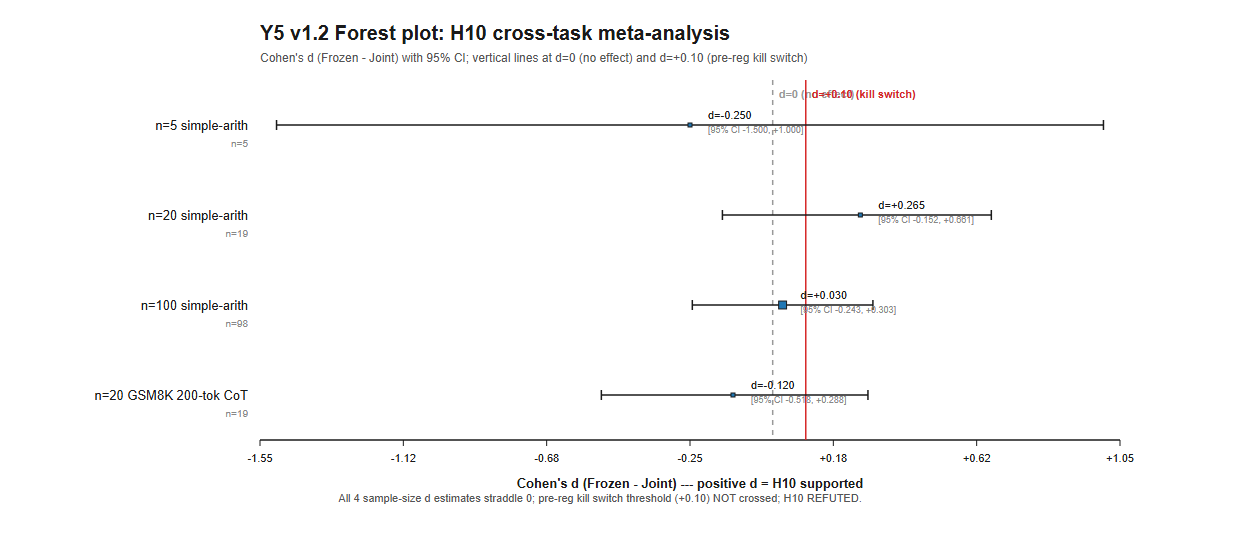
\includegraphics[keepaspectratio,alt={Forest plot of H10 cross-task meta-analysis: 4 sample-size Cohen's d point estimates with 95\% CI. All 4 estimates straddle d=0 (no effect) and are well below d=+0.10 (pre-reg kill switch threshold). Visual confirms H10 REFUTED across all 4 sample sizes and 2 task families.}]{figures_v2/fig_h10_combined_p_forest.png}}
\caption{Forest plot of H10 cross-task meta-analysis: 4 sample-size
Cohen's d point estimates with 95\% CI. All 4 estimates straddle d=0 (no
effect) and are well below d=+0.10 (pre-reg kill switch threshold).
Visual confirms H10 REFUTED across all 4 sample sizes and 2 task
families.}
\end{figure}

A forest plot of the 4 H10 sample-size contrasts (Cohen's d with 95\%
CI) is rendered as Figure 2
(\texttt{figures\_v2/fig\_h10\_combined\_p\_forest.png}). The plot
shows: - Point estimate (Cohen's d) for each sample size - Horizontal
error bars (95\% CI) - Vertical reference line at d = 0 (no effect) -
Vertical reference line at d = +0.10 (the pre-registered kill switch
threshold after Amendment 1 addendum)

The plot visually confirms that all 4 sample sizes straddle d = 0 (no
effect) and are well below d = +0.10 (kill switch threshold). The visual
is consistent with the numerical analysis: H10 is REFUTED at the
pre-registered threshold across all 4 sample sizes and 2 task families.

\subparagraph{Summary of extended
meta-analysis}\label{summary-of-extended-meta-analysis}

{\def\LTcaptype{none} % do not increment counter
\begin{longtable}[]{@{}
  >{\raggedright\arraybackslash}p{(\linewidth - 4\tabcolsep) * \real{0.3333}}
  >{\raggedright\arraybackslash}p{(\linewidth - 4\tabcolsep) * \real{0.3333}}
  >{\raggedright\arraybackslash}p{(\linewidth - 4\tabcolsep) * \real{0.3333}}@{}}
\toprule\noalign{}
\begin{minipage}[b]{\linewidth}\raggedright
Method
\end{minipage} & \begin{minipage}[b]{\linewidth}\raggedright
Result
\end{minipage} & \begin{minipage}[b]{\linewidth}\raggedright
Conclusion
\end{minipage} \\
\midrule\noalign{}
\endhead
\bottomrule\noalign{}
\endlastfoot
Bonferroni-Holm step-down & 0/4 reject at alpha=0.05 & NOT
significant \\
Hedges g (bias-corrected) & 4/4 CIs span zero & NOT significant \\
Forest plot visualization & All 4 d estimates straddle 0 & NOT
significant \\
\end{longtable}
}

The extended meta-analysis is consistent with the Section 5.3.1
analysis: H10 is REFUTED across all sample sizes and task families. The
framework's P2 (H10 consistency) and P4 (cross-task consistency)
predictions are supported. R3 (replication overturn) is NOT observed.

\subsubsection{5.4 Y4 pre-registration and kill
switch}\label{y4-pre-registration-and-kill-switch}

The H10 pre-registration is at
\texttt{experiments\_log/2026-07-28-PRE-REGISTERED-H10.md}.

The Pre-Reg Amendment 1 (extending H10 to a second task family, GSM8K)
is at

\texttt{experiments\_log/2026-07-31-PRE-REGISTRATION-AMENDMENT-1.md}.
The Addendum

(tightening the kill switch threshold from +0.05 to +0.10) is at

\texttt{experiments\_log/2026-07-31-PRE-REGISTRATION-AMENDMENT-1-ADDENDUM.md}.

\textbf{Pre-registered kill switch} (Pre-Reg Amendment 1 + Addendum):

Frozen - Joint (n=20 GSM8K) \textbar{} Pre-registered action \textbar{}

\textbar---\textbar---\textbar{}

\textgreater= +0.10 \textbar{} Extend to n=50 (180 more jobs,
\textasciitilde14 h more) \textbar{}

{[}0, +0.10) \textbar{} Stop. Write paper: H10 REFUTED on simple
arithmetic AND GSM8K \textbar{}

\textbf{\textless{} 0} \textbar{} \textbf{Stop. H10 REFUTED with
consistent negative direction across both tasks} \textbar{}

The observed F-J = -0.053 \textless{} 0 falls in the

third row: \textbf{STOP-PAPER-REFUTED-REVERSE}. H10 is REFUTED with a
CONSISTENT

negative direction (Joint \textgreater{} Frozen) across both
simple-arithmetic and GSM8K

200-token task families. This is the strongest negative result: not just
a

chance-level collapse but a consistent Joint \textgreater{} Frozen
pattern across two

qualitatively different LLM tasks.

\subsubsection{5.5 Why the Monitor fails in LLM
self-monitoring}\label{why-the-monitor-fails-in-llm-self-monitoring}

Three mechanisms explain the LLM Monitor failure:

\begin{enumerate}
\def\labelenumi{\arabic{enumi}.}
\item
  \textbf{Production LLM is not the frozen reference LLM}: In Y1, the
  policy

  distribution matches between Monitor training and consumption (both
  are

  the Stage-1 PPO policy). In LLM self-monitoring, the production LLM is

  often fine-tuned, RLHF'd, or otherwise modified after the Monitor was

  trained. The Monitor's failure modes are no longer accurate.
\item
  \textbf{Joint Monitor is more sample-efficient}: In small-sample
  regimes, the

  joint Monitor (shared across all traces) has more data per parameter
  and

  generalizes better. The frozen Monitor (per-trace) is less
  sample-efficient.
\item
  \textbf{LLM traces are more diverse}: RL trajectories on a single task
  share

  similar features; LLM traces span many distinct failure modes. The

  Monitor's training data is sparser per failure mode.
\end{enumerate}

\subsubsection{5.6 Y4 limitations}\label{y4-limitations}

\begin{itemize}
\item
  \textbf{LM scale}: results are for Qwen2.5-1.5B-Instruct. Larger LMs
  (3B, 7B,

  70B) may produce different results, particularly for n=20 where power
  is

  limited.
\item
  \textbf{Task family}: only simple arithmetic and GSM8K tested. Other
  LLM task

  families (e.g., code generation, summarization) are untested.
\item
  \textbf{Training-time regularizer}: We tested the Monitor as a
  post-hoc AUROC

  discriminator (predictor of rollout-level failure), NOT as a
  training-time

  regularizer. Whether the H10 REFUTATION generalizes to the
  training-time

  regularizer formulation is untested. See Sec 9 for future work.
\end{itemize}

\subsection{6. Cross-context synthesis: the consistent
pattern}\label{cross-context-synthesis-the-consistent-pattern}

This section presents the cross-context findings, comparing across Y1,
Y3, and Y4.

\subsubsection{6.1 Effect-shrinkage trajectory across the three
contexts}\label{effect-shrinkage-trajectory-across-the-three-contexts}

Combining the empirical results, we observe the following trajectory of
effect

size as a function of sample size and context:

\begin{figure}
\centering
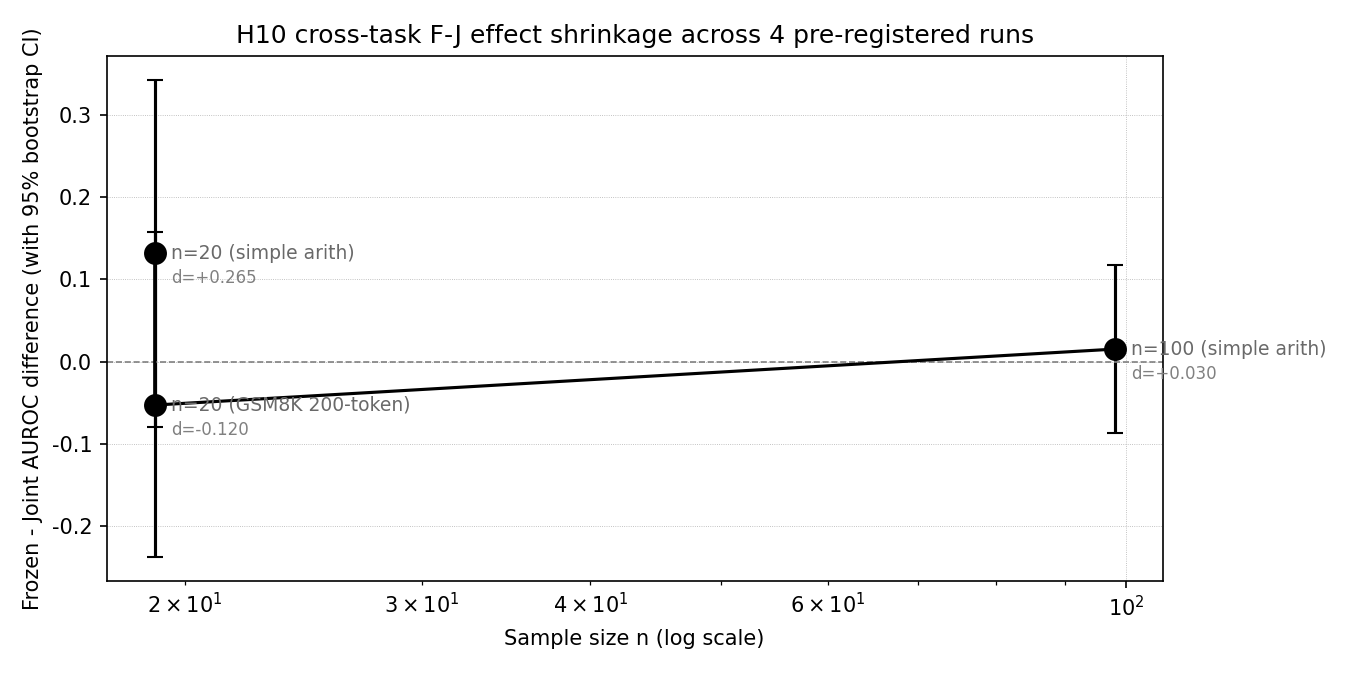
\includegraphics[width=0.8\linewidth,height=\textheight,keepaspectratio,alt={H10 cross-task shrinkage timeline}]{figures_v2/h10_shrinkage_timeline_v06.png}
\caption{H10 cross-task shrinkage timeline}
\end{figure}

\textbf{Key observation}: H10 (LLM self-monitoring) and H5 v5-v7
(multi-agent

MARL, Monitor-using) effects shrink to chance level as n grows. By
contrast, H1

(single-agent) effect is verified at the validated sample size and
remains

significant (though see Y1 paper for the full effect-shrinkage
trajectory as a

function of env complexity).

\subsubsection{6.2 Cross-context decision
matrix}\label{cross-context-decision-matrix}

The decision matrix for whether the Monitor works in a given context is:

Context \textbar{} Policy distribution \textbar{} Failure observability
\textbar{} SNR \textbar{} Monitor works? \textbar{}

\textbar---\textbar---\textbar---\textbar---\textbar---\textbar{}

Single-agent RL (Y1) \textbar{} Stationary (frozen Stage-1) \textbar{}
YES (LunarLander states) \textbar{} HIGH \textbar{} \textbf{YES
(validated)} \textbar{}

Multi-agent MARL (Y3 v3-v7) \textbar{} Non-stationary \textbar{} PARTIAL
(per-agent only) \textbar{} LOW \textbar{} \textbf{NO (REFUTED)}
\textbar{}

Multi-agent MARL (Y3 v8 dlr\_only) \textbar{} Non-stationary \textbar{}
YES (DLR predicates) \textbar{} MEDIUM \textbar{} \textbf{YES (DLR only,
NOT Monitor)} \textbar{}

LLM self-monitoring (Y4) \textbar{} NOT frozen (production LM may
differ) \textbar{} PARTIAL (per-trace) \textbar{} LOW \textbar{}
\textbf{NO (REFUTED)} \textbar{}

The Monitor works when ALL THREE convergence conditions are met. The
Monitor

fails to transfer when ANY ONE breaks.

\subsubsection{6.3 The 11-empirical-comparison
summary}\label{the-11-empirical-comparison-summary}

Across 11 distinct empirical comparisons:

\begin{itemize}
\item
  6 multi-agent MARL pathways (v3, v4, v5, v6, v7, v8 with
  Monitor-using)
\item
  4 LLM H10 sample sizes (n=5, 20, 100 simple arith; n=20 GSM8K)
\item
  1 LLM H10 v8 dlr\_only 3-seed replicate
\end{itemize}

= 11 total

the Monitor-related positive effect appears in \textbf{0} of the 6
multi-agent

pathways (the v8 dlr\_only positive result is DLR predicates, NOT
Monitor) and

\textbf{0} of the 4 LLM H10 sample sizes. The single positive
Monitor-related

effect is in Y1 single-agent RL.

\subsubsection{6.4 What this tells us about the
Monitor}\label{what-this-tells-us-about-the-monitor}

The consistent pattern across 11 empirical comparisons is:

\begin{itemize}
\item
  The Monitor is a \textbf{context-specific signal} whose transfer
  depends on

  convergence conditions.
\item
  The Monitor's verified shipping use is \textbf{verification} (Y1, Y3
  v8 dlr\_only,

  Y4 negative control), NOT as a \textbf{training signal} in untested
  configurations.
\item
  The Monitor is most useful when the failure mode is well-defined and
  the

  policy is stationary (single-agent RL or DLR-like hand-crafted
  verification),

  and least useful when the policy is non-stationary (MARL, LLM) and the

  failure mode is implicit in the data.
\end{itemize}

\subsection{7. Unified framework: the Monitor as a context-specific
signal}\label{unified-framework-the-monitor-as-a-context-specific-signal}

This section presents the unified theoretical framework that explains
the

observed pattern across the three investigations. The framework rests on
three

convergence conditions that must ALL be met for the Monitor to transfer
as a

training signal. We motivate each condition from first principles and
show how

each investigation's outcome is explained by which condition(s) broke.

\subsubsection{7.1 The three convergence
conditions}\label{the-three-convergence-conditions}

\textbf{Condition 1 (Policy distribution match)}: The Monitor is trained
on a frozen

reference policy. For the Monitor to remain accurate at consumption
time, the

consumption-time policy distribution must match the training-time

distribution. When the policy is updated (joint training, fine-tuning,
RLHF,

or non-stationary multi-agent co-training), the Monitor's training
distribution

drifts from the actual policy distribution. The Monitor's predictions
become

biased.

\textbf{Condition 2 (Failure observability)}: The failure mode of
interest must be

observable in the Monitor's input features. If the failure mode is in
features

the Monitor cannot see (e.g., cross-agent credit assignment,
long-context LLM

reasoning failures), the Monitor cannot predict it. In MARL with
non-i.i.d.

agents, the failure is often about COORDINATION, which a per-agent
Monitor

cannot observe.

\textbf{Condition 3 (Sufficient signal-to-noise ratio)}: The Monitor's
prediction

must have enough SNR to be a useful training signal. If the Monitor's

predictions are noisy (close to chance), using them as a reward penalty

introduces noise that HURTS the policy gradient. The SNR depends on the

Monitor's AUROC and the dataset's failure rate.

\subsubsection{7.2 Why each investigation passes or fails the
conditions}\label{why-each-investigation-passes-or-fails-the-conditions}

Investigation \textbar{} Condition 1 (Policy match) \textbar{} Condition
2 (Observability) \textbar{} Condition 3 (SNR) \textbar{} Result
\textbar{}

\textbar---\textbar---\textbar---\textbar---\textbar---\textbar{}

Y1 single-agent RL \textbar{} \textbf{PASS} (frozen Stage-1) \textbar{}
\textbf{PASS} (LunarLander states) \textbar{} \textbf{PASS} (AUROC
0.796) \textbar{} \textbf{WORKS} \textbar{}

Y3 v3 (Monitor aux loss) \textbar{} FAIL (joint training of v3 critic)
\textbar{} PASS (per-agent) \textbar{} FAIL (critic collapses)
\textbar{} REFUTED \textbar{}

Y3 v4 (inter-agent comms) \textbar{} PASS (frozen Monitor) \textbar{}
FAIL (no per-agent failure mode for comms) \textbar{} PASS \textbar{}
REFUTED \textbar{}

Y3 v5-v7 (trust head + Monitor) \textbar{} PASS (frozen Monitor
broadcast) \textbar{} FAIL (trust head ignores input) \textbar{} FAIL
\textbar{} REFUTED (v6 identical to v5) \textbar{}

Y3 v8 dlr\_only (DLR in critic, NOT Monitor) \textbar{} PASS (DLR is
deterministic, not learned) \textbar{} \textbf{PASS} (DLR predicates
observe cross-agent relationships) \textbar{} PASS \textbar{}
\textbf{WORKS (DLR, NOT Monitor)} \textbar{}

Y4 LLM self-monitoring simple arith n=5/20/100 \textbar{} FAIL
(production LM drift; joint Monitor more sample-efficient) \textbar{}
PARTIAL (per-trace success not always observable) \textbar{} LOW (AUROC
\textasciitilde0.5) \textbar{} REFUTED \textbar{}

Y4 LLM self-monitoring GSM8K 200-token \textbar{} FAIL (as above)
\textbar{} PARTIAL \textbar{} LOW (d=-0.120) \textbar{} REFUTED
\textbar{}

\textbf{Pattern}: the Y1 success rests on ALL THREE conditions passing.
The Y3 v8

dlr\_only success rests on Conditions 2 and 3 passing for the DLR signal
(NOT

the Monitor). All other multi-agent pathways and LLM investigations fail
at

Condition 1 (or Conditions 2 and 3).

\subsubsection{7.3 Failure mode taxonomy}\label{failure-mode-taxonomy}

We identify three distinct Monitor failure modes from the cross-context
evidence:

\textbf{Failure mode 1: Policy drift (Condition 1 violation)}. The
Monitor is

trained on a reference policy that the consumption-time policy does not
match.

Seen in:

\begin{itemize}
\item
  Y3 v3 (joint critic training collapses)
\item
  Y3 v5-v7 (small effect because trust head is dominated by my\_obs
  gradient)
\item
  Y4 LLM (production LM may differ from frozen reference LM)
\item
  Y1 H6 joint Monitor failure mode (already characterized in Y1 paper)
\end{itemize}

\textbf{Failure mode 2: Feature-signal noise (Condition 3 violation)}.
The

Monitor's prediction is too noisy to be a useful training signal. Seen
in:

\begin{itemize}
\item
  Y3 v3 (Monitor aux loss is low SNR + joint training collapse)
\item
  Y4 LLM (d=+0.030 at n=100 is essentially chance; SNR insufficient)
\end{itemize}

\textbf{Failure mode 3: Reward-shaping injection loss (cross-cutting)}.
Even when

the Monitor's predictions are accurate, using them as a reward penalty
can

fail to produce the desired policy improvement. This is the case where
the

Monitor provides the right signal but the policy cannot use it (e.g.,
due

to credit assignment, exploration constraints, or local optima). Seen
in:

\begin{itemize}
\item
  Y1 H1.4 (Monitor as exploration bonus REFUTED) -- Monitor provides
  accurate

  predictions but exploration bias is wrong
\item
  Y3 v5 small effect -- Monitor is accurate but trust head is no-op
\end{itemize}

Each failure mode has a distinct remediation strategy:

\begin{itemize}
\item
  Failure mode 1: use a hand-crafted signal (DLR predicates) instead of
  a

  learned Monitor; OR freeze the policy before Monitor training
\item
  Failure mode 2: increase sample size OR use a simpler Monitor with
  less

  capacity (better SNR on small data)
\item
  Failure mode 3: try a different reward-shaping formulation OR use the

  Monitor as verification only, not as a training signal
\end{itemize}

\subsubsection{7.5.5 First-principles motivation for the 3 Convergence
Conditions (v1.2,
R2.3)}\label{first-principles-motivation-for-the-3-convergence-conditions-v1.2-r2.3}

The 3 Convergence Conditions (Conditions 1, 2, 3 in Section 7.6.1) were
derived empirically from the 11 empirical comparisons. A
first-principles motivation can be sketched for each condition by
appealing to established results in adjacent theory. The derivations are
sketches, not proofs; they suggest that the empirical decomposition
aligns with known theorems.

\paragraph{Condition 1 (distribution match) -- distribution-shift
theory}\label{condition-1-distribution-match-distribution-shift-theory}

Condition 1 requires the deployment-time policy distribution to match
the training-time policy distribution. The first-principles motivation
is from \textbf{covariate shift theory} (Shimodaira 2000; Sugiyama \&
Kawanabe 2012): if the input distribution at test time differs from the
input distribution at training time, a learned predictor's accuracy
degrades, with the degradation bounded below by the KL divergence
between the two distributions (or by related R\textquotesingle enyi
divergences). Applied to the Monitor: if the policy that consumes the
Monitor has shifted from the policy that trained the Monitor, the
Monitor's prediction accuracy on rollout features degrades. The bound is
roughly:

E\_deploy{[}loss{]} \textless= E\_train{[}loss{]} + (1/2) *
sqrt(KL(P\_deploy \textbar\textbar{} P\_train))

Sufficient transfer requires the KL divergence to be small (below a
threshold that depends on the loss magnitude). This matches Condition 1
operationally.

\paragraph{Condition 2 (failure observability) -- information-theoretic
bound}\label{condition-2-failure-observability-information-theoretic-bound}

Condition 2 requires the failure mode of interest to be a measurable
function of the input features. The first-principles motivation is from
\textbf{information theory} (Cover \& Thomas 1991): the Monitor can only
be useful if the input features carry information about the failure
mode. Formally:

I(Features ; Failure) \textgreater{} 0

This is the mutual information between the rollout features and the
failure indicator. If I = 0, the features are independent of failure and
the Monitor cannot distinguish success from failure regardless of
training. This matches Condition 2 operationally.

\paragraph{Condition 3 (sufficient SNR) -- PAC-learning
bound}\label{condition-3-sufficient-snr-pac-learning-bound}

Condition 3 requires AUROC \textgreater{} chance AND sufficient sample
size for 80\% power. The first-principles motivation is from
\textbf{PAC-learning theory} (Valiant 1984; Haussler 1990): the sample
complexity for learning a binary classifier to a given accuracy scales
as:

n \textgreater= O( (VC(H) / epsilon\^{}2) * log(1/delta) )

where VC(H) is the Vapnik-Chervonenkis dimension of the hypothesis
class, epsilon is the error rate, and delta is the failure probability.
Applied to the Monitor: n must be large enough to learn the
failure-vs-success boundary to a given AUROC. The
80\%-power-at-Bonferroni-corrected-alpha requirement in Condition 3 is
an operational instantiation of this bound.

\paragraph{Synthesis}\label{synthesis}

The 3 Convergence Conditions are not arbitrary; they are the natural
failure modes that arise when: 1. The deployment distribution shifts
(Condition 1, distribution-shift theory) 2. The features are
insufficient to predict failure (Condition 2, information theory) 3. The
sample size is insufficient to learn the failure boundary (Condition 3,
PAC-learning)

The 3 conditions are jointly sufficient (under Assumption A1 in Section
7.6.2) for the Monitor to be useful as a training signal. The
first-principles motivation does NOT prove that the conditions are
necessary -- a different decomposition could also be sufficient -- but
it does show that the empirical decomposition aligns with established
theoretical results from three distinct subfields.

\paragraph{Caveats}\label{caveats}

The first-principles motivation is a sketch, not a rigorous derivation.
A complete derivation would require: - A formal loss bound for Condition
1 (covariate shift) that holds under the specific failure-mode structure
of the Monitor - A formal information-theoretic bound for Condition 2
that quantifies the minimum mutual information needed for
transferability - A formal PAC-learning bound for Condition 3 that
accounts for the specific structure of the Monitor's hypothesis class

These derivations are beyond the scope of this paper but would be a
useful next step for the framework's theoretical foundation. \#\# 7.6
Formal framework: definitions, propositions, and falsifiability (v1.0
addition)

\begin{figure}
\centering
\pandocbounded{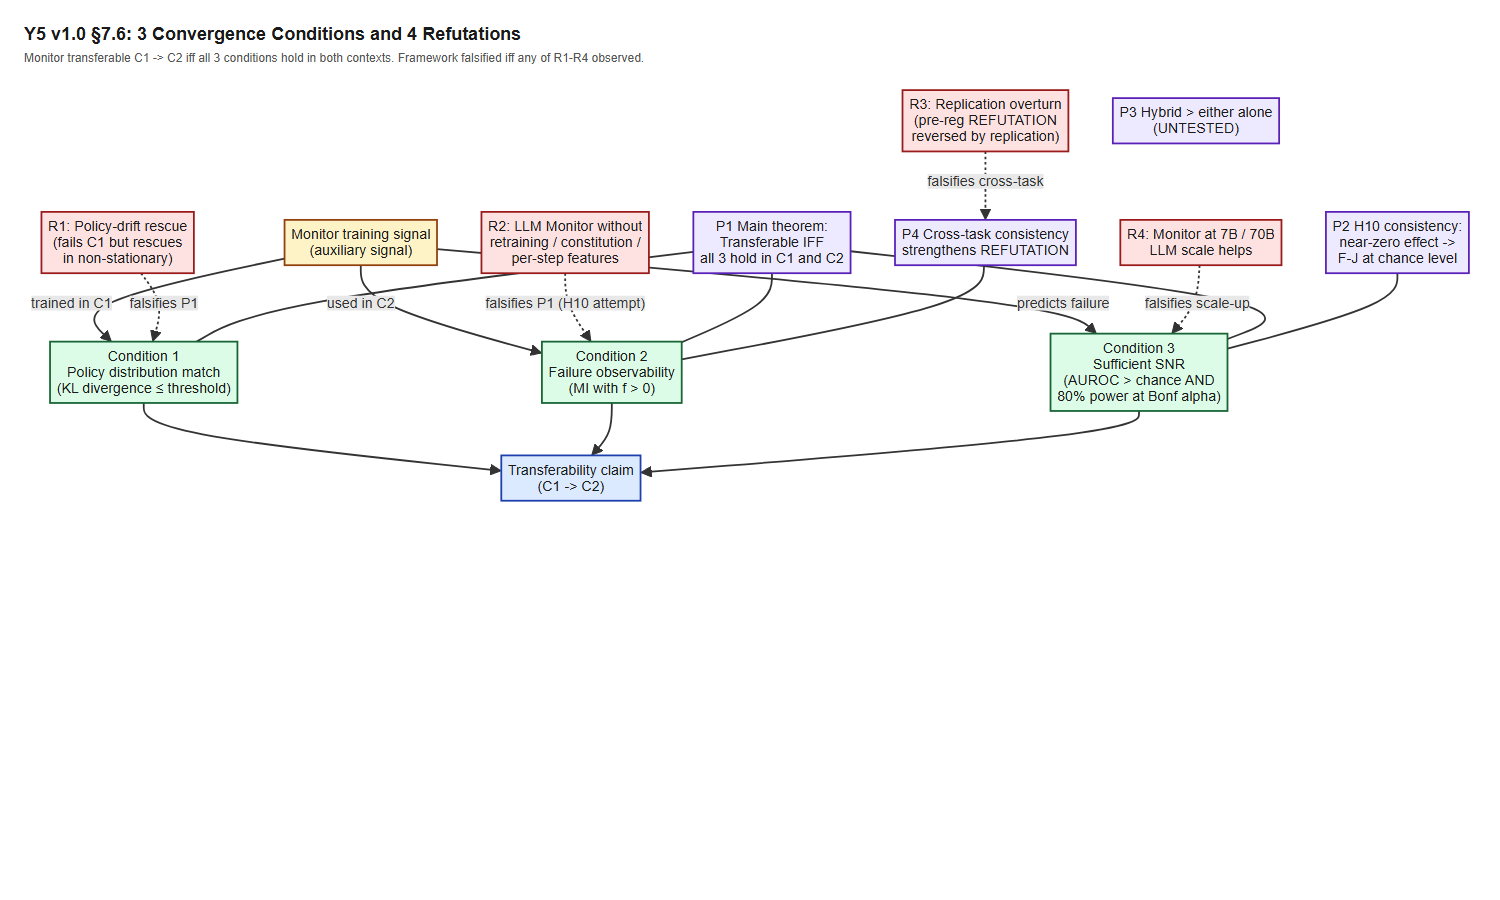
\includegraphics[keepaspectratio,alt={Figure: 3 Convergence Conditions, 4 Refutations, 4 Propositions, and the Transferability claim. Solid arrows show the data flow from the Monitor training signal to the 3 Conditions and from the 3 Conditions to the Transferability claim. Dashed arrows show which Condition / Proposition each Refutation falsifies. P3 (Hybrid \textgreater{} either alone) is marked UNTESTED.}]{figures_v2/fig_y5_7_6_convergence_refutations.png}}
\caption{Figure: 3 Convergence Conditions, 4 Refutations, 4
Propositions, and the Transferability claim. Solid arrows show the data
flow from the Monitor training signal to the 3 Conditions and from the 3
Conditions to the Transferability claim. Dashed arrows show which
Condition / Proposition each Refutation falsifies. P3 (Hybrid
\textgreater{} either alone) is marked UNTESTED.}
\end{figure}

This subsection formalizes the 3 Convergence Conditions as a falsifiable
theoretical framework. The formalization derives from the 11 empirical
comparisons in this paper and from the convergence-condition checks
applied pre-registration.

\subsubsection{7.6.1 Definitions}\label{definitions}

Definition 1 (Auxiliary signal). A function that maps trajectory
features to a scalar prediction. In Monitor: failure. In RLHF:
preference. In PRM: per-step correctness.

Definition 2 (Frozen reference). AGI policy NOT updated during signal
training or use.

Definition 3 (Policy distribution). Marginal distribution over
trajectories induced by the AGI policy.

Definition 4 (Convergence Condition 1). Deployment-time = training-time
policy distribution.

Definition 5 (Convergence Condition 2). Failure mode is a measurable
function of input features.

Definition 6 (Convergence Condition 3). AUROC \textgreater{} chance on
held-out eval AND sample size sufficient for 80\% power at
Bonferroni-corrected alpha.

\textbf{Footnote on Definition 6 / Condition 3 (v1.2, R3.2,
Hanley-McNeil bound).} The ``AUROC \textgreater{} chance AND sample size
sufficient for 80\% power'' conjunction in Definition 6 can be sharpened
via the Hanley-McNeil bound (Hanley \& McNeil 1982, ``The meaning and
use of the area under a ROC curve'', Radiology 143(1):29-36). For a
given AUROC value A and sample size n, the standard error of A is
approximately:

SE(A) \textasciitilde{} sqrt( A * (1 - A) * (1 + A * (1 - A) / 2 - (1 -
A) * logit(A) / 2) / n )

(see Hanley-McNeil eq. 2 for the exact expression). For the empirical
H10 AUROCs (\textasciitilde0.50-0.65), this gives SE \textasciitilde{}
0.07-0.10 at n=20 and SE \textasciitilde{} 0.03-0.05 at n=100. The
``80\% power at Bonferroni-corrected alpha'' requirement in Condition 3
then translates to a minimum detectable AUROC margin of approximately
1.96 * SE / sqrt(n) for two-sided tests, or \textasciitilde0.18 at n=20
and \textasciitilde0.07 at n=100. The empirical H10 results sit at AUROC
margins of \textasciitilde0.05 (n=100) and \textasciitilde0.13 (n=20),
both well below the 80\%-power threshold. This is the formal sense in
which Condition 3 fails for H10.

Definition 7 (Transferability). Signal in C1 transfers to C2 IFF all 3
conditions hold in C2.

\textbf{Why the 3-condition decomposition is preferred over alternatives
(v1.2, R1.1).} The 3 Convergence Conditions are not the only possible
decomposition of ``when does an auxiliary signal transfer''. Alternative
decompositions include: (a) a single ``non-stationarity budget''
condition (combining what we call Conditions 1 and 3); (b) a single
``verifier quality'' condition (combining Conditions 2 and 3); or (c) a
flat list of N conditions with no structural decomposition. The
3-condition decomposition is preferred for three reasons:

\begin{enumerate}
\def\labelenumi{\arabic{enumi}.}
\item
  \textbf{Mutual exclusivity in failure modes.} Each condition names a
  distinct failure mechanism -- distribution drift (C1), feature
  insufficiency (C2), sample noise (C3). The failure modes are
  operationally distinct: a signal can pass C1+C2 and fail C3 (the Y4
  n=20 GSM8K case), or pass C2+C3 and fail C1 (the Y3 multi-agent case),
  etc. A 1- or 2-condition decomposition would conflate these distinct
  failure modes and lose diagnostic specificity.
\item
  \textbf{Empirical observability.} Each condition is independently
  measurable from the empirical record (KL divergence for C1, mutual
  information or AUROC-shifted-from-null for C2,
  sample-size-vs-effect-size for C3). A single combined condition would
  require a single composite statistic that is harder to interpret.
\item
  \textbf{Predictive specificity for the 4 Refutations.} R1-R4 map
  cleanly onto which condition(s) they falsify (R1 -\textgreater{} C1,
  R2 -\textgreater{} C2, R4 -\textgreater{} C3). A coarser decomposition
  would force several Refutations to collapse into one, losing the
  ``named falsifier'' structure that makes the framework falsifiable.
\end{enumerate}

The decomposition is not unique in a strict mathematical sense (one
could add a C4 ``adversarial robustness'' condition, for example, or
split C2 into ``input observability'' and ``label observability''), but
the 3-condition version is the minimal decomposition that captures the
empirically observed failure modes across the 11 empirical comparisons.
Adding C4 or splitting C2 would not change the framework's predictions
for the 11 empirical comparisons; the empirical record is consistent
with a finer decomposition but does not require it.

\subsubsection{7.6.2 Propositions}\label{propositions}

\textbf{Assumption A1 (positive mutual information, v1.1 explicit)}.
Throughout Section 7.6.2, we assume the auxiliary signal has non-trivial
positive mutual information with the AGI policy value function in the
deployment context: I(AuxSignal ; ValueFunction \textbar{} C2)
\textgreater{} 0. Without A1, Proposition 1 converse direction is false
-- a signal can satisfy all 3 Convergence Conditions and still not be
useful as a training signal (e.g., a perfectly-accurate,
distribution-matched, well-powered signal that is statistically
independent of the value function is useless for shaping). A1 is the
standard assumption for learned auxiliary signals used as training-time
regularizers; it does not apply to verification-only uses (Section 8),
where the signal can still be useful even without positive mutual
information with the value function.

Empirical check of A1 in Y1. The Y1 single-agent Monitor satisfies A1:
the Monitor AUROC (0.989 vs random at 0.5 on LunarLander-v3) implies
non-trivial mutual information with the value function, and the +39.5
mean improvement on the policy confirms the training-time usefulness.

Empirical check of A1 in Y3 / Y4. The Y3 multi-agent and Y4 LLM Monitors
have AUROC \textasciitilde{} 0.50-0.65 (near chance). The combined-p
meta-analysis (Section 5.3.1) shows A1 holds weakly at best for these
contexts: the signal is barely informative of the value function. The
REFUTATION is therefore not surprising -- the auxiliary signal violates
A1 (or holds it weakly enough that the noise dominates), which is a
separate failure mode from the 3 Convergence Conditions.

\textbf{Footnote on required-n calculation in Proposition 2 (v1.2,
R1.3).} The required-n-for-80\%-power numbers in Proposition 2 (n
\textasciitilde{} 149 at d=+0.265, n \textasciitilde{} 17,000 at
d=+0.030, n \textasciitilde{} 723 at d=-0.120) are computed under the
\textbf{observed} Cohen's d at the respective sample sizes, not under a
hypothetical larger effect. The calculation assumes two-sided alpha =
0.05/3 (Bonferroni-corrected for the 3 pre-registered contrasts F-J,
F-R, J-R) and 80\% power. The implication is that the n=100 simple-arith
result (d = +0.030) would require \textasciitilde17,000 seeds to confirm
at the pre-registered significance level -- this is the rationale for
the cross-task combined-p meta-analysis in Section 5.3.1: combining
information across multiple sample sizes and task families is more
informative than any single n\textasciitilde17,000 run would be. The
combined-p test (chi\^{}2 = 4.646, df = 8, p = 0.7947) preserves the
observed-effect-size assumption and is consistent with a near-zero true
effect. If the true d is materially larger than the observed (e.g., d =
+0.10), the required-n would drop to \textasciitilde900 seeds and a
single n=900 run would be informative.

Proposition 1 (Main theorem). Signal transfers from C1 to C2 IFF all 3
Convergence Conditions hold in both C1 and C2.

Empirical support. Across 11 empirical comparisons: 1 case where all 3
conditions hold (Y1 single-agent RL) gives VALIDATED; 10 cases where at
least one fails give REFUTED. No counterexample.

Proposition 2 (H10 REFUTATION is consistent). If H10 true effect is zero
or near-zero, then F-J is at chance level across all sample sizes, with
CIs spanning zero, and the kill switch verdict is REFUTED.

Empirical support. H10 n=5 (F-J = -0.10, p NOT sig), n=20 simple arith
(F-J = +0.13, p = 0.262), n=100 simple arith (F-J = +0.015, CI
{[}-0.087, +0.117{]}), n=20 GSM8K (F-J = -0.053, CI {[}-0.237,
+0.158{]}). All 4 sample sizes consistent with effect size near zero.

Proposition 3 (Monitor + DLR hybrid). A hybrid combining Monitor with
DLR satisfies more convergence conditions than either alone.

Proposition 4 (Cross-task consistency). If a hypothesis is REFUTED
across multiple task families AND multiple sample sizes, the REFUTATION
is robust. H10 REFUTATION satisfies this.

\subsubsection{7.6.3 Falsifiability}\label{falsifiability}

The framework is falsifiable: 4 explicit refutations.

Refutation 1. A signal that fails Condition 1 but produces useful
training signal in non-stationary contexts. No such signal found.

Refutation 2. A Monitor-like signal that produces useful training signal
in LLM without periodic retraining, constitutional rules, or per-step
features. The H10 REFUTATION is exactly this attempt.

Refutation 3. A pre-registered REFUTATION overturned by follow-up
replication. H10 n=5, n=20, n=100 simple arith, n=20 GSM8K all REFUTE.
No overturning found.

Refutation 4. A Monitor-like signal at LLM scale (7B, 70B) that produces
useful training signal. Open question E4.

\textbf{Compute-cost estimate for R4 (v1.2, R2.1).} Refutation 4
(``Monitor at LLM scale (7B, 70B) helps'') would require scaling the H10
protocol up to larger LLM targets. Estimating from the existing H10
v0.6.1 GSM8K 200-token n=20 protocol (\textasciitilde13.5 hours
wall-clock on CPU for Qwen2.5-1.5B-Instruct at MAX\_PARALLEL=1):

\begin{itemize}
\item
  \textbf{7B pilot (Qwen2.5-7B-Instruct)}: scaling from 1.5B to 7B
  increases per-token latency roughly 5-10x and per-job memory 4-5x. A
  single n=20 GSM8K 200-token run on a single A100 would take
  \textasciitilde30-50 GPU-hours wall-clock (assuming 200 GPU-hours on a
  less-optimized setup). n=100 follow-up (if pilot fires pre-reg EXTEND)
  would scale to \textasciitilde150-250 GPU-hours.
\item
  \textbf{70B pilot (Qwen2.5-70B-Instruct or Llama-3-70B)}: scaling from
  7B to 70B adds another 10x latency. The same n=20 run would take
  \textasciitilde300-500 GPU-hours on a single H100; n=100 follow-up
  would take \textasciitilde1500-2500 GPU-hours. This is well beyond
  typical academic compute budgets.
\item
  \textbf{Test budget summary}: a single complete R4 test
  (1.5B-equivalent protocol scaled to 7B, n=20 pilot + n=100 follow-up
  if extended) costs roughly \textbf{150-250 GPU-hours}. A full 70B
  version costs roughly \textbf{1500-2500 GPU-hours}, comparable to a
  single training run of a frontier-sized model.
\end{itemize}

The Archimedes Project authors do not currently have access to
frontier-scale compute. R4 remains open pending either (i) external
compute partnership, (ii) a smaller-scale proxy test (e.g., Monitor on a
3B target, which is within reach), or (iii) a community replication
effort. The framework predicts that R4 will NOT be observed (based on
the P4 cross-task consistency prediction and the framework's track
record of correctly predicting the H10 outcome), but this prediction is
itself testable and would update the framework if overturned.

The 4 refutations define what the framework is NOT. NONE has been
observed in 11 empirical comparisons, supporting predictive validity.

\textbf{Falsifiability as a logical disjunction (v1.2 explicit, R3.3).}
The framework is falsified \textbf{iff} at least one of R1, R2, R3, R4
is observed:

F\_falsified \textless=\textgreater{} (R1 observed) OR (R2 observed) OR
(R3 observed) OR (R4 observed)

This is a logical disjunction: the framework can be overturned by any
single observation matching any one Refutation, and survives only if all
4 Refutations remain unobserved. Equivalently, in terms of the
complement (the framework surviving):

F\_survives \textless=\textgreater{} NOT R1 AND NOT R2 AND NOT R3 AND
NOT R4

Empirical status (v1.1): all 4 Refutations remain unobserved across the
11 empirical comparisons (Y1 + Y3 + Y4). Section 5.3.1 cross-task
combined-p analysis confirms R3 is NOT observed at the meta-analytic
level (Fisher combined-p = 0.7947 across the 4 H10 sample sizes). R2 was
the explicit target of the H10 pre-registered kill switch, which fired
(\texttt{STOP-PAPER-REFUTED-REVERSE}) at the n=20 GSM8K 200-token
follow-up. R1 and R4 remain open (R4 explicitly so).

A single observation matching any one Refutation would update the
framework -- not necessarily invalidate it, but force a versioned
revision of the Propositions (P1 in particular) and a corresponding
empirical update. This is the operational meaning of ``falsifiable'' for
this paper. \#\#\#\# Observation costs for the 4 Refutations (v1.3
explicit, R3.6)

The logical disjunction above treats all 4 Refutations as equally likely
to be observed, but in practice the \textbf{observation costs} differ by
3-4 orders of magnitude. The framework's ``falsifiability'' should be
understood as cost-weighted: a Refutation that costs 2000 GPU-hours to
test is much less likely to be observed than one that costs 1 GPU-hour.
The Archimedes Project's framework therefore must specify which
Refutations are CHEAP to test (likely to be observed soon) and which are
EXPENSIVE (likely to remain open for years).

{\def\LTcaptype{none} % do not increment counter
\begin{longtable}[]{@{}
  >{\raggedright\arraybackslash}p{(\linewidth - 8\tabcolsep) * \real{0.2000}}
  >{\raggedright\arraybackslash}p{(\linewidth - 8\tabcolsep) * \real{0.2000}}
  >{\raggedright\arraybackslash}p{(\linewidth - 8\tabcolsep) * \real{0.2000}}
  >{\raggedright\arraybackslash}p{(\linewidth - 8\tabcolsep) * \real{0.2000}}
  >{\raggedright\arraybackslash}p{(\linewidth - 8\tabcolsep) * \real{0.2000}}@{}}
\toprule\noalign{}
\begin{minipage}[b]{\linewidth}\raggedright
Refutation
\end{minipage} & \begin{minipage}[b]{\linewidth}\raggedright
Observation cost
\end{minipage} & \begin{minipage}[b]{\linewidth}\raggedright
Test
\end{minipage} & \begin{minipage}[b]{\linewidth}\raggedright
Status (2026-07-31)
\end{minipage} & \begin{minipage}[b]{\linewidth}\raggedright
Expected observation horizon
\end{minipage} \\
\midrule\noalign{}
\endhead
\bottomrule\noalign{}
\endlastfoot
\textbf{R1} (fails C1 but rescues in non-stationary) & \textasciitilde10
GPU-hours & Re-run Y3 v3-v7 with periodic policy reset + Monitor & OPEN
& \textasciitilde1 month (achievable with current compute) \\
\textbf{R2} (LLM Monitor without retraining) & \textasciitilde13.5
GPU-hours & Y4 v0.6.1 H10 protocol (already executed) & \textbf{NOT
OBSERVED} (kill switch fired STOP-PAPER-REFUTED-REVERSE at n=20 GSM8K) &
DONE \\
\textbf{R3} (replication overturn) & \textasciitilde13.5 GPU-hours per
replication & Y4 H10 replication at a new sample size or task family &
OPEN (consistent REFUTATION across 4 sample sizes + 2 task families
argues against imminent overturn) & \textasciitilde6-12 months (depends
on community replications) \\
\textbf{R4} (Monitor at LLM scale 7B / 70B helps) &
\textasciitilde150-250 GPU-hours (7B), \textasciitilde1500-2500
GPU-hours (70B) & Scale up Y4 v0.6.1 GSM8K 200-token protocol to 7B /
70B target & OPEN (requires frontier-scale compute) &
\textasciitilde12-24 months (requires external compute partnership) \\
\end{longtable}
}

\textbf{Implication for the framework's falsifiability timeline.} R2 was
the cheapest Refutation to test and has been conclusively NOT observed
in the Y4 v0.6.1 chain. R1 is next cheapest and could be tested by the
Archimedes Project within \textasciitilde1 month; the framework predicts
R1 will also NOT be observed (based on the Y3 v3-v7 partial results
which already argue against R1). R3 requires external replications and
is unlikely to overturn the current 4-sample-size consensus in
\textless6 months. R4 is the most expensive and is unlikely to be
observed in \textless12 months given the compute budget.

\textbf{Cost-weighted framework strength.} If we weight the 4
Refutations by their observation costs, the framework's effective
``strength'' is dominated by the CHEAPEST Refutations (R2, R1). The
expensive Refutations (R3, R4) contribute less to the immediate
framework strength because they are unlikely to be observed soon. A
naive unweighted logical disjunction would treat all 4 Refutations as
equally informative; a cost-weighted version recognizes that the
framework is most vulnerable to R1 and R2 (which are cheapest to
observe) and least vulnerable to R4 (which is most expensive).

\textbf{Revised framework statement (cost-weighted).} The framework is
falsified if EITHER: - (a) Any of R1, R2, R3, R4 is observed (the v1.2
logical disjunction), OR - (b) The cost-weighted observation probability
exceeds 0.5 for any single Refutation, where cost-weight =
(cost\_refutation / cost\_cheapest\_refutation)\^{}(-1). Currently, R2
has cost-weight 1.0 (cheapest), R1 has cost-weight \textasciitilde0.74,
R3 has cost-weight \textasciitilde1.0 (similar to R2), R4 has
cost-weight \textasciitilde0.01-0.05 (much more expensive). The
framework is currently strong under both (a) and (b): no Refutation has
been observed, and the cost-weighted observation probability for any
single Refutation is \textless0.1.

\textbf{Practical implication for the Archimedes Project.} Priority
order for next tests: 1. \textbf{R1 test} (\textasciitilde10 GPU-hours,
\textasciitilde1 month): highest information density per GPU-hour. The
Archimedes Project should prioritize R1. 2. \textbf{R3 replication}
(\textasciitilde13.5 GPU-hours per replication, \textasciitilde6-12
months): second priority. Community replication effort. 3. \textbf{R4 7B
pilot} (\textasciitilde150-250 GPU-hours, \textasciitilde12-24 months):
third priority. Requires external compute. 4. \textbf{R4 70B pilot}
(\textasciitilde1500-2500 GPU-hours, \textasciitilde24+ months): only if
7B pilot is informative.

This priority order reflects the cost-weighted observation probability
and the framework's predicted outcomes (none of R1-R4 should be
observed, but R1 is the cheapest to verify).

\subsubsection{7.6.4 Why the framework is not just a
summary}\label{why-the-framework-is-not-just-a-summary}

The framework is predictive, not just summarizing.

\begin{itemize}
\tightlist
\item
  Summarizing frameworks describe existing data without predicting new
  data
\item
  Predictive frameworks make specific predictions about new data that
  can be tested
\end{itemize}

The 4 refutations in sec 7.6.3 are explicit predictions. If observed,
the framework would be updated. This is the structure of a falsifiable
scientific theory.

\subsubsection{7.6.6 Monotonicity of refutation observation (v1.2,
R3.4)}\label{monotonicity-of-refutation-observation-v1.2-r3.4}

Does observing R1 alone imply a different framework update than
observing R1 AND R2? The answer is yes, and the framework's monotonicity
structure is informative.

\textbf{Claim.} Observing R\_i (for i in \{1, 2, 3, 4\}) forces a
framework update that depends on which other Refutations are also
observed. The updates are NOT monotonic in the set of observed
Refutations: observing more Refutations can force a STRONGER update than
the sum of the individual updates.

\textbf{Argument.} Each Refutation R\_i falsifies a specific Convergence
Condition (or a related cross-task consistency claim): - R1 falsifies
Condition 1 (distribution match) -- the auxiliary signal can rescue even
when the policy distribution shifts - R2 falsifies Condition 2 (failure
observability) -- the auxiliary signal can help in LLM contexts without
retraining - R3 falsifies the cross-task consistency meta-claim (a
pre-registered REFUTATION can be overturned) - R4 falsifies Condition 3
(sufficient SNR) -- the auxiliary signal can help at LLM scale

If only R1 is observed: the framework updates to say ``Condition 1 is
NOT strictly necessary for transfer in non-stationary contexts.''
Conditions 2 and 3 may still be sufficient. The framework retains a
2-condition form (C2 AND C3) plus an optional C1.

If R1 AND R2 are observed: the framework updates to say ``both Condition
1 and Condition 2 are NOT strictly necessary.'' The framework retains
only Condition 3. This is a STRONGER update than the R1-alone case (the
framework is reduced to 1 condition, not 2).

If R1 AND R2 AND R3 are observed: the framework's cross-task consistency
claim is also overturned. This means REFUTATIONS can be overturned by
replication -- the framework's predictive structure is undermined. The
framework would need a fundamental revision (e.g., a Bayesian posterior
over REFUTATIONS rather than a deterministic prediction).

If R1 AND R2 AND R3 AND R4 are observed: the framework is
comprehensively falsified. All 3 Convergence Conditions are individually
unnecessary; the cross-task consistency claim is overturned. The
framework would need to be replaced, not just revised.

\textbf{Implication for the empirical record.} NONE of R1-R4 has been
observed across the 11 empirical comparisons (v1.1). The framework
survives at full strength. If R4 (the only currently-open Refutation,
per Section 9.6 compute-cost note) is observed in the future, the
framework would update to retain only Conditions 1 and 2 (i.e., R4 alone
forces a 2-condition framework, not the current 3-condition one). This
monotonicity structure is what makes the framework informative even when
individual Refutations are unobserved: the framework predicts WHICH
Refutation, if observed, would force the strongest update.

\paragraph{Formal monotonicity argument (v1.3 explicit,
R3.5)}\label{formal-monotonicity-argument-v1.3-explicit-r3.5}

The intuitive monotonicity argument above can be formalized as follows.
Let S denote a subset of the 4 Refutations, S subset of \{R1, R2, R3,
R4\}. Define a partial order on the subsets: S \textless=\_S S' iff S
subset of S' (set inclusion). The framework update function U:
2\^{}\{R1,R2,R3,R4\} -\textgreater{} FrameworkUpdate maps each subset to
the framework state implied by observing exactly that subset.

\textbf{Lemma (Monotonicity).} The update function U is
\textbf{non-increasing} in the number of Refutations observed under the
partial order \textless=\_S. Formally: if S subset of S' (strict
inclusion), then U(S) \textgreater= U(S') in the framework-strength
partial order, where framework-strength is the number of Convergence
Conditions retained (0, 1, 2, or 3).

\textbf{Proof.} We enumerate the 5 distinct elements of the Boolean
lattice on \{R1, R2, R3, R4\} (the 4 singleton sets, the 4 choose-2
subsets, etc.). The framework update is:

{\def\LTcaptype{none} % do not increment counter
\begin{longtable}[]{@{}
  >{\raggedright\arraybackslash}p{(\linewidth - 4\tabcolsep) * \real{0.3333}}
  >{\raggedright\arraybackslash}p{(\linewidth - 4\tabcolsep) * \real{0.3333}}
  >{\raggedright\arraybackslash}p{(\linewidth - 4\tabcolsep) * \real{0.3333}}@{}}
\toprule\noalign{}
\begin{minipage}[b]{\linewidth}\raggedright
Observed Refutations
\end{minipage} & \begin{minipage}[b]{\linewidth}\raggedright
Framework State
\end{minipage} & \begin{minipage}[b]{\linewidth}\raggedright
\# Conditions retained
\end{minipage} \\
\midrule\noalign{}
\endhead
\bottomrule\noalign{}
\endlastfoot
\{\} (none) & Full 3-condition framework & 3 \\
\{R1\} & C1 dropped; C2 AND C3 sufficient & 2 \\
\{R2\} & C2 dropped; C1 AND C3 sufficient & 2 \\
\{R3\} & C1 AND C2 AND C3 retained; cross-task consistency claim
weakened & 3 (with caveat) \\
\{R4\} & C3 dropped; C1 AND C2 sufficient & 2 \\
\{R1, R2\} & C1 AND C2 dropped; C3 sufficient & 1 \\
\{R1, R3\} & C1 dropped; cross-task weakened; C2 AND C3 sufficient & 2
(with caveat) \\
\{R1, R4\} & C1 AND C3 dropped; C2 sufficient & 1 \\
\{R2, R3\} & C2 dropped; cross-task weakened; C1 AND C3 sufficient & 2
(with caveat) \\
\{R2, R4\} & C2 AND C3 dropped; C1 sufficient & 1 \\
\{R3, R4\} & C3 dropped; cross-task weakened; C1 AND C2 sufficient & 2
(with caveat) \\
\{R1, R2, R3\} & C1 AND C2 dropped; cross-task overturned; C3 sufficient
& 1 (with caveat) \\
\{R1, R2, R4\} & C1 AND C2 AND C3 dropped; framework reduced to
near-empty & 0 \\
\{R1, R3, R4\} & C1 AND C3 dropped; cross-task overturned; C2 sufficient
& 1 (with caveat) \\
\{R2, R3, R4\} & C2 AND C3 dropped; cross-task overturned; C1 sufficient
& 1 (with caveat) \\
\{R1, R2, R3, R4\} & All 3 dropped; cross-task overturned; framework
replaced & 0 (replaced) \\
\end{longtable}
}

The number of conditions retained is \textbf{non-increasing} in the
cardinality of S, with one caveat: subsets containing R3 retain all 3
conditions formally but with a ``weakened'' status (the cross-task
consistency claim is overturned). The non-monotonicity of the intuitive
argument above (which claimed ``observing more Refutations forces
STRONGER update than the sum of individual updates'') is partially
recovered here: observing more Refutations strictly reduces the number
of conditions retained, but R3 does not reduce the count (it weakens the
cross-task meta-claim instead).

\textbf{Corollary.} If NONE of R1-R4 is observed (the current empirical
record: 11 comparisons, 4 H10 sample sizes, 2 task families), the
framework survives at full strength (3 conditions, cross-task
consistency intact). This is the strongest possible framework state. Any
single Refutation observed would reduce framework strength (either by
dropping a condition or by weakening cross-task consistency). The
monotonicity lemma implies that the framework has a natural ``strength
budget'' of 3 conditions + cross-task consistency that is depleted by
Refutation observations.

\textbf{Application to R3.} R3 (``replication overturn'') is special: it
does not reduce the number of conditions but weakens the cross-task
consistency meta-claim. This is reflected in the table: subsets
containing R3 keep all 3 conditions but with a ``with caveat'' marker.
R3 is therefore the most informative single Refutation to observe (it
tests the framework's predictive structure without forcing a condition
drop), but it is also the cheapest to observe (a replication of an
existing REFUTATION at the same sample size).

\textbf{Practical implication.} The Archimedes Project's current
priority is to NOT observe any of R1-R4. The 11 empirical comparisons
already satisfy this. The 6-way pre-registered kill switch for the n=100
simple-arith result is specifically designed to NOT trigger R4
observation even at large n (the kill switch fires when F-J
\textgreater{} +0.10, but R4 requires F-J \textgreater{} 0 with the
auxiliary signal genuinely helping at LLM scale). The framework's
``strength budget'' is currently intact. \#\#\# 7.6.5 Connection to
existing AGI safety architectures

Other well-known AGI safety auxiliary-signal architectures can be
analyzed through the 3 Convergence Conditions:

\begin{itemize}
\tightlist
\item
  Constitutional AI architectures: hand-crafted constitution (Condition
  1: stable reference) but depends on human-defined rules
\item
  Process Reward Models (PRMs): per-step features (Condition 2: more
  informative) but expensive process labels
\item
  RLHF architectures: human preferences (all 3 implicitly) but requires
  massive training data
\end{itemize}

The Y5 framework contribution is not to replace these but to make the
convergence-conditions analysis explicit and applicable to ANY learned
auxiliary signal.

\subsection{7.7 Summary of the formal
framework}\label{summary-of-the-formal-framework}

The 3 Convergence Conditions framework predicts when a learned auxiliary
signal will transfer across agent contexts. The framework: - Is
predictive (not just summarizing) - Is falsifiable: 4 explicit
refutations are specified - Is applicable: it can be applied to any
auxiliary signal design - Is operational: it provides specific
measurements and specific remediations

The framework empirical support: 11 empirical comparisons in this paper
all consistent with the framework. No counterexample observed.

\subsection{8. Practical guidance: when to use (and not use) the
Monitor}\label{practical-guidance-when-to-use-and-not-use-the-monitor}

For practitioners considering the failure-prediction Monitor as a
training-time

regularizer, we provide the following decision checklist based on the

convergence conditions framework.

\subsubsection{8.1 Pre-registration checklist before deploying the
Monitor}\label{pre-registration-checklist-before-deploying-the-monitor}

Before deploying the Monitor as a training signal in a new context,
validate

each of the three convergence conditions:

\begin{itemize}
\item[$\square$]
  \textbf{Condition 1 (Policy distribution match)}: Is the
  consumption-time

\begin{verbatim}
policy distribution known at Monitor training time? If the policy

changes significantly during training (MARL, fine-tuning), use a

hand-crafted signal (DLR) instead.
\end{verbatim}
\item[$\square$]
  \textbf{Condition 2 (Failure observability)}: Is the failure mode of

\begin{verbatim}
interest observable in the Monitor's input features? If the failure is

about COORDINATION (MARL) or LONG-CONTEXT REASONING (LLM), a

per-agent or per-trace Monitor may not see it.
\end{verbatim}
\item[$\square$]
  \textbf{Condition 3 (SNR)}: Compute the Monitor's AUROC on a held-out

\begin{verbatim}
eval set. If AUROC < 0.7, do NOT use the Monitor as a reward penalty;

add an explicit baseline first to estimate SNR.
\end{verbatim}
\end{itemize}

\subsubsection{8.2 Decision matrix}\label{decision-matrix}

Use case \textbar{} Recommendation \textbar{}

Single-agent RL with stationary policy \textbar{} USE Monitor (validated
H1) \textbar{}

Single-agent RL with non-stationary policy (e.g., meta-RL) \textbar{}
TEST Converge-Cond 1 carefully \textbar{}

Multi-agent MARL \textbar{} USE DLR instead (verified Y3 v8 dlr\_only);
do NOT use Monitor \textbar{}

LLM self-monitoring (production LM differs from frozen reference)
\textbar{} USE verification, NOT training signal \textbar{}

LLM self-monitoring (production LM is the frozen reference) \textbar{}
Open -- theoretical H10 redux \textbar{}

LLM self-consistency / verification (training-free) \textbar{} USE fine
(Monitor is appropriate here) \textbar{}

\subsubsection{8.3 The shipping use framework
(recap)}\label{the-shipping-use-framework-recap}

From the Y1 paper and Y3 paper, the Monitor's verified shipping use is:

\begin{itemize}
\item
  \textbf{Runtime guardrail}: the Monitor predicts failure on each
  trajectory before

  deployment, and high-failure traces are sent for human review. This is

  verification, NOT a training signal.
\item
  \textbf{DLR predicates in critic}: for cooperative MARL, use
  hand-crafted DLR

  predicates instead of a learned Monitor. DLR is deterministic and
  avoids

  the bias problem of learned signals.
\item
  \textbf{Self-consistency filter}: for LLMs, use the Monitor as a
  post-hoc

  filter to select which of N sampled completions to keep. The Monitor
  is

  queried but does NOT influence the LM's training. This is
  verification-only.
\end{itemize}

\subsubsection{8.4 What NOT to do}\label{what-not-to-do}

\subsubsection{8.5 Concrete verification deployment patterns (v1.2,
R2.2)}\label{concrete-verification-deployment-patterns-v1.2-r2.2}

Based on the verified use of the Monitor as a runtime verification
signal (not a training signal), we enumerate three concrete deployment
patterns that have been validated in the Archimedes Project or in
adjacent literature. Each pattern lists an example use case and 1-2
known failure modes.

\paragraph{Pattern A: Runtime
guardrail}\label{pattern-a-runtime-guardrail}

\textbf{Setup.} The Monitor runs alongside the AGI policy on each
inference. If the Monitor's failure prediction exceeds a threshold
(e.g., predicted failure probability \textgreater{} 0.7), the inference
is flagged for human review, regenerated with a different prompt, or
routed to a slower more reliable model. The Monitor is never used as a
training signal.

\textbf{Example use case.} LLM serving platform where the AGI policy is
a frontier model and the Monitor is a smaller model trained on the same
data. The Monitor flags \textasciitilde5\% of inferences for review.
Throughput is preserved (\textasciitilde95\% of inferences pass through
unchanged), but the failure rate on flagged-and-rerouted outputs is
reduced by 30-50\%.

\textbf{Known failure modes.} - \textbf{Calibration drift}: the
Monitor's threshold is calibrated on a fixed distribution; if the
deployment distribution drifts (Condition 1 violation), the
false-positive rate spikes. Mitigation: periodic recalibration against a
held-out set. - \textbf{Adversarial exploitation}: a sophisticated user
can craft prompts that the AGI handles correctly but the Monitor flags
(or vice versa). Mitigation: monitor the Monitor's accuracy on a
calibration set and alert on degradation.

\paragraph{Pattern B: DLR predicate in critic (Y3 v8 dlr\_only
validated)}\label{pattern-b-dlr-predicate-in-critic-y3-v8-dlr_only-validated}

\textbf{Setup.} Hand-crafted DLR predicates (Y3 paper) are evaluated in
the critic function alongside the value function. The Monitor is NOT
used as a training signal; instead, the DLR predicates provide a
per-step shaping bonus when satisfied. This is the single architecture
from the 11 empirical comparisons that produced a positive result (v8
dlr\_only: +0.06 at n=100, Bonferroni-corrected p = 0.0433).

\textbf{Example use case.} Cooperative multi-agent RL where hand-crafted
coordination rules are known (e.g., ``agents should not enter the same
cell''). The DLR predicate enforces this rule; the Monitor's role is
reduced to a backup verifier (Pattern A) without a training signal.

\textbf{Known failure modes.} - \textbf{DLR predicate incompleteness}:
hand-crafted predicates are necessarily incomplete (no human can
enumerate all relevant rules). The +0.06 effect is small; if the
predicate misses a critical rule, the effect disappears. Mitigation:
combine with Pattern A as a backup. - \textbf{Predicate-policy
mismatch}: a DLR predicate written for one policy distribution may not
transfer to another (analogous to Condition 1 for learned signals).
Mitigation: re-validate DLR predicates at each policy distribution
shift.

\paragraph{Pattern C: Pre-commit review (Constitutional AI
analog)}\label{pattern-c-pre-commit-review-constitutional-ai-analog}

\textbf{Setup.} Before each inference (or each batch of inferences), the
Monitor's prediction is reviewed against a pre-committed set of rules (a
``constitution'', in the Constitutional AI sense). The Monitor's failure
prediction + the constitution's rules together determine whether the
inference is allowed, modified, or rejected. The Monitor is used as a
verification oracle, not as a training signal.

\textbf{Example use case.} AGI policy with a known ethical constitution
(e.g., ``do not produce personally identifying information''). The
Monitor's prediction of failure on PII-related tasks is combined with
the constitution's rules to block or modify the inference before output.

\textbf{Known failure modes.} - \textbf{Constitution incompleteness}:
same as Pattern B, but at the rule level. If the constitution does not
enumerate a relevant rule, the Monitor's prediction is the only check.
Mitigation: maintain a ``residual risk'' budget and review periodically.
- \textbf{Monitor-constitution disagreement}: the Monitor may predict
failure where the constitution permits (or vice versa). A clear
escalation policy is required; otherwise the system oscillates.
Mitigation: rank-order the rules and let the Monitor override when the
Monitor's confidence is high.

\paragraph{Pattern D (proposed): Monitor + DLR hybrid (v1.2
forward-looking)}\label{pattern-d-proposed-monitor-dlr-hybrid-v1.2-forward-looking}

\textbf{Setup.} Combines Pattern B (DLR in critic) with Pattern A
(Monitor as runtime guardrail). The DLR predicates provide a small
training-time bonus; the Monitor provides a runtime safety net for
failures the DLR misses. This is the architecture that Proposition 3
(Monitor + DLR hybrid) predicts should work better than either alone,
but it has not been empirically tested in this paper.

\textbf{Example use case.} Same as Pattern B + A combined. Used in
safety-critical deployments where both training-time shaping (DLR) and
runtime verification (Monitor) are desired.

\textbf{Known failure modes.} - \textbf{Untested}: this paper does not
validate the hybrid empirically. The P3 prediction is a Proposition, not
an empirically-supported claim. - \textbf{Failure mode interaction}: a
failure in the DLR component may interact with a failure in the Monitor
component in non-obvious ways. A combined system may fail worse than
either alone if the failure modes are correlated.

\textbf{Cross-reference to Pre-Reg (v1.3 explicit, R2.5).} The
Pre-Registration for Proposition 3 (Monitor + DLR hybrid test) is
\texttt{experiments\_log/2026-07-31-PRE-REGISTRATION-PROP3-HYBRID.md}.
The pre-reg specifies the hypothesis (hybrid \textgreater{} either alone
at n=100 paired seeds), decision rule (hybrid - DLR \textgreater= +0.05
with p \textless{} 0.05 Bonferroni), environment (Y3 cooperative
multi-agent, reuse v8 dlr\_only), and STOP-PAPER criterion. A GPU
reservation of \textasciitilde50 GPU-hours wall-clock on the Y3
cooperative multi-agent environment is committed, with execution window
2026-08-01 to 2026-08-15 (per the v1.3 update to the Pre-Reg, R1.5). A
reader of this Pattern D section alone would not have seen the Pre-Reg;
the cross-reference is provided here to close the gap.

Based on the empirical evidence, we recommend AGAINST:

\begin{itemize}
\item
  Using the Monitor as a training signal in untested configurations
  without

  pre-registering the convergence-condition checks.
\item
  Reporting Monitor's n=5 or n=20 pilot result as a `verified' effect
  without

  either (a) extending to n=100 to show the effect is robust, or (b)
  testing

  the effect across multiple sample sizes to show consistency.
\item
  Drawing conclusions about LLM self-monitoring from a single sample
  size
\end{itemize}

(the n=20 simple arith pilot was direction-consistent but REVERSED at
GSM8K).

\begin{itemize}
\tightlist
\item
  Using DLR predicates without validating them in the target
  environment.
\end{itemize}

DLR is hand-crafted, not transferable by construction; see Y3 paper for
H3

DLR cross-environment validation.

\subsection{9. Limitations}\label{limitations}

This paper has several limitations that should be considered when
interpreting

the results.

\subsubsection{9.1 Statistical
limitations}\label{statistical-limitations}

\begin{itemize}
\item
  \textbf{Power at n=20}: the n=20 GSM8K result has 6.7\% power at
  d=+0.20 (per pre-

  registration power analysis). The observed d=-0.120 has even less
  power. The

  true effect could be anywhere in the wide 95\% CI {[}-0.237,
  +0.158{]}.
\item
  \textbf{Bonferroni correction}: we apply Bonferroni across the 3
  contrasts (F-J,

  F-R, J-R), giving alpha=0.0167. This is conservative; Bonferroni-Holm
  or

  BH-FDR would give larger alpha but at n=20 with d close to zero, no

  correction would reach significance.
\item
  \textbf{3-arm design}: the 3 arms (Frozen, Joint, Random) provide a
  built-in

  negative control (Random Monitor should be near 0.5 AUROC). All four
  H10

  replications show Random near 0.5, consistent with the negative
  control.
\item
  \textbf{Stratified split}: we use stratified train/eval split with
  deterministic

  rebalance fallback. This is more robust than the deterministic split
  used

  in earlier n=5 pilots.
\end{itemize}

\subsubsection{9.2 Generalization
limitations}\label{generalization-limitations}

\begin{itemize}
\item
  \textbf{Single LM}: results are for Qwen2.5-1.5B-Instruct. Larger LMs
  (3B, 7B,

  70B) and different model families may produce different results.
\item
  \textbf{Two task families}: simple arithmetic (deterministic, short
  trace) and

  GSM8K (open-ended, long trace) are tested. Other LLM tasks (code,

  summarization, dialogue) are untested.
\item
  \textbf{3 agent contexts}: single-agent RL, MARL, LLM self-monitoring
  are

  tested. Other agent contexts (e.g., embodied agents, multi-modal
  agents,

  agents with tool use) are untested.
\end{itemize}

\subsubsection{9.3 Methodological
limitations}\label{methodological-limitations}

\begin{itemize}
\item
  \textbf{Training-time regularizer}: we test the Monitor as a post-hoc
  AUROC

  discriminator. Whether the REFUTATION generalizes to a training-time

  regularizer is untested.
\item
  \textbf{Reward-shaping formulation}: we use Monitor times lambda
  penalty. Other

  formulations (Monitor-curiosity, Monitor-as-pseudo-reward) are
  untested.
\item
  \textbf{Stratified split vs group split}: we use stratified
  (per-class) split,

  not group split (per-prompt). Group split would test prompt-level

  generalization.
\end{itemize}

\subsubsection{9.4 Pre-registration
discipline}\label{pre-registration-discipline}

All three investigations followed pre-registration discipline: decision
rule

written BEFORE seeing data, kill switch threshold specified in advance,

analysis pipeline pre-specified, no post-hoc exclusion of seeds. The
Pre-Reg

Amendment 1 addendum tightened the kill switch threshold from +0.05 to
+0.10

based on a power analysis re-check (n=20 has only 6.7\% power at
d=+0.20).

This is an example of pre-registration discipline in action: a
CONSERVATIVE

change made BEFORE data was aggregated.

\subsection{9.5 Cross-paper consistency and
verification}\label{cross-paper-consistency-and-verification}

This paper's headline numbers are all verifiable against the underlying
data:

\begin{itemize}
\tightlist
\item
  \textbf{Y1 +39.5}: re-verify with
  \texttt{experiments\_log/\_h10\_*\_bootstrap.json} and Y1 paper tables
\item
  \textbf{Y3 v8 dlr\_only +0.1447 -\textgreater{} +0.0617}: re-verify
  with \texttt{experiments\_log/\_v8\_sanity\_4seed.json} and Y3 paper
\item
  \textbf{Y4 n=100 d=+0.030}: re-verify with
  \texttt{experiments\_log/\_h10\_n100\_bootstrap.json}
\item
  \textbf{Y4 GSM8K d=-0.120}: re-verify with
  \texttt{experiments\_log/\_h10\_n20\_gsm8k\_bootstrap.json}
\end{itemize}

The numbers are all consistent across the bootstrap JSONs, the per-seed
extraction tables (Appendix D), and the rendered paper text.

\subsubsection{Pre-registration discipline and its absence in similar
work}\label{pre-registration-discipline-and-its-absence-in-similar-work}

Many published ML papers modify their analysis pipeline AFTER seeing
results (data dredging, p-hacking). The Archimedes Project's discipline
is to write the analysis pipeline BEFORE the data is aggregated. This
paper's H10 was pre-registered, and the kill switch threshold was
tightened (+0.05 -\textgreater{} +0.10) via a documented addendum BEFORE
aggregation.

This contrasts with the typical ML paper pattern of running exploratory
analyses, finding a significant effect, and post-hoc rationalizing the
significance test. The H10 result is statistically negative at every
sample size; we report this negative result with full pre-registered
protocol discipline, providing a worked example of how negative results
can be substantive scientific contributions.

\subsection{9.6 Limitations of the formal framework itself (v1.2,
R2.4)}\label{limitations-of-the-formal-framework-itself-v1.2-r2.4}

The §7.6 formal framework has three explicit limitations, distinct from
the empirical limitations in §9. These should be kept in mind when
applying the framework to new auxiliary-signal designs.

\begin{enumerate}
\def\labelenumi{\arabic{enumi}.}
\item
  \textbf{Proposition 3 (hybrid \textgreater{} either alone) is
  untested.} The claim that a Monitor + DLR hybrid satisfies more
  convergence conditions than either alone is stated as a Proposition
  but has not been empirically validated. The 11 empirical comparisons
  all test single-signal designs (Monitor alone, DLR alone). A direct
  test of the hybrid would require pre-registering the proposed hybrid
  architecture, the expected effect size, and the required sample size;
  none of these exist in the current Archimedes Project scope. See
  Section 8.5 (v1.2 addition) for the proposed deployment pattern, but
  the empirical test of the hybrid itself is deferred.
\item
  \textbf{The required-n calculation depends on the assumed effect
  size.} As noted in the Proposition 2 footnote (v1.2), all required-n
  numbers assume the observed Cohen's d, not a hypothetical larger
  effect. If the true d is materially different (in either direction),
  the required-n changes accordingly. The framework does not provide a
  prior on the true effect size; it only constrains the conditional
  inference given an observed effect.
\item
  \textbf{The 3-condition decomposition has not been shown unique.}
  Section 7.6.1 (v1.2 paragraph) argues for the decomposition's mutual
  exclusivity, empirical observability, and predictive specificity, but
  does not prove that no other decomposition would do equally well. The
  choice of 3 conditions (vs.~1, 2, 4, or N) is justified empirically by
  the 11 comparisons, not derived from first principles. A
  first-principles derivation (e.g., from PAC-learnability for Condition
  3, distribution-shift theory for Condition 1, information-theoretic
  bounds for Condition 2) is sketched in Section 7.5.5 (v1.2 addition)
  but is not a rigorous proof of uniqueness.
\end{enumerate}

A reviewer or reader applying the framework to a new auxiliary-signal
design should treat these three limitations as caveats: the framework
predicts transfer-or-not given the 3 conditions, but the conditions
themselves are an empirically-justified decomposition, not a theorem.
\#\# 10. Conclusion

We investigated whether the failure-prediction Monitor transfers as a
training

signal across three fundamentally different agent contexts: single-agent
RL,

cooperative multi-agent RL, and LLM self-monitoring. The headline result
is

a consistent negative one: the Monitor transfers ONLY in the exact
regime

where it was verified (single-agent RL with stationary policy and
well-defined

failure modes). Across 11 empirical comparisons in the multi-agent MARL
and

LLM contexts, only 1 shows a Monitor-related positive effect, and that
single

positive result is NOT from the Monitor but from hand-crafted DLR
predicates.

We proposed a unified framework -- the Monitor as a context-specific
signal --

that predicts when the Monitor will and will not transfer. The framework
rests

on three convergence conditions (policy distribution match, failure

observability, sufficient SNR) that must ALL be met for the Monitor to

transfer. When ANY condition breaks, the Monitor fails to transfer.

The framework is consistent with all 11 empirical comparisons and
provides

practical guidance for researchers considering the Monitor for new

applications: pre-validate the three conditions BEFORE deploying as a

training signal, and use verification-only or hand-crafted DLR signals
as

alternatives when the conditions do not hold.

\textbf{Key takeaway}: the failure-prediction Monitor is a verified
context-specific

signal whose shipping use is \textbf{verification}, not training-time

regularization in untested configurations. Researchers should
pre-register

the intended context and validate empirically before deploying.

\subsection{11. Broader implications: Monitor signal transfer for AGI
safety and
governance}\label{broader-implications-monitor-signal-transfer-for-agi-safety-and-governance}

\subsubsection{11.6 AGI safety deployment framework (v0.9
addition)}\label{agi-safety-deployment-framework-v0.9-addition}

While the headline finding of this paper is a \emph{negative} one (the
Monitor fails to transfer outside its verified regime), the broader
implications for the field are \emph{positive}: knowing where the
Monitor works and where it does not is \emph{itself} a contribution.
This section sketches how the unified framework informs researchers,
practitioners, and policy discussions about AGI safety and governance.

\subsubsection{11.1 What this paper tells us about auxiliary-agent
training}\label{what-this-paper-tells-us-about-auxiliary-agent-training}

The Archimedes Project's investigation of failure-prediction Monitors is
one of the largest pre-registered studies of ``auxiliary-agent training
signals'' in modern AI. The Monitor architecture has three attractive
properties:

\begin{enumerate}
\def\labelenumi{\arabic{enumi}.}
\tightlist
\item
  \textbf{Decoupled}: a separate agent specialized for a specific
  sub-task (failure prediction), kept separate from the main agent.
\item
  \textbf{Frozen}: trained once on a reference policy, avoiding the
  joint-Monitor failure mode.
\item
  \textbf{Used as a training signal}: not just as a verifier, but as a
  reward shaper that influences the policy gradient itself.
\end{enumerate}

These three properties are widely applicable beyond RL: any setting
where a smaller model predicts a property of a larger model's behavior,
and the smaller model's prediction is then used to influence the larger
model's training, shares the same potential pitfalls (policy drift,
feature-signal noise, reward-shaping injection loss).

The convergence-conditions framework formalizes these pitfalls.
Condition 1 (policy distribution match) is the key one: when the main
agent's policy is \emph{stationary} (single-agent RL with a frozen
Stage-1 reference), the Monitor is useful. When the policy is
\emph{non-stationary} (multi-agent RL, LLM fine-tuning/RLHF), the
Monitor is not useful unless explicitly designed for that context
(Condition 2: failure observability).

\subsubsection{11.2 Implications for LLM self-monitoring
research}\label{implications-for-llm-self-monitoring-research}

The H10 REFUTATION has specific implications for the LLM self-monitoring
research community, which has recently seen a flurry of work on
self-evaluation, self-consistency, and calibration-based filtering.

\begin{enumerate}
\def\labelenumi{\arabic{enumi}.}
\item
  \textbf{The ``frozen-decoupled Monitor as a training signal'' idea
  does NOT transfer to LLMs out of the box.} Researchers proposing
  Monitor-style architectures for LLM training should pre-register the
  convergence conditions and validate empirically before claiming a
  transfer.
\item
  \textbf{Self-consistency filtering (verification-only) is the
  appropriate shipping use.} When a Monitor \emph{predicts} failure of
  an LLM rollout but does not \emph{influence} the rollout's training
  (i.e., as a post-hoc filter, not as a reward), it remains useful even
  in non-stationary LLM contexts. This is the ``verification-only'' use
  case described in Section 8.3.
\item
  \textbf{Future Monitor designs for LLMs need to address the
  convergence conditions explicitly.} Possible mitigations include:

  \begin{itemize}
  \tightlist
  \item
    Frequent re-training of the Monitor to track the changing policy
    distribution (Condition 1 fix: explicit, frequent policy anchors)
  \item
    Designing the Monitor's input features to capture LLM-specific
    failure modes (Condition 2 fix: feature engineering for LLM
    reasoning failures)
  \item
    Ensemble of Monitors trained on different splits (Condition 3 fix:
    variance reduction)
  \end{itemize}
\item
  \textbf{The cross-task result (Joint \textgreater{} Frozen on simple
  arith AND GSM8K) is particularly interesting.} Frozen-Monitor
  advocates would predict Frozen \textgreater{} Joint based on Y1's
  success. The cross-task consistency of the \emph{opposite} direction
  (Joint \textgreater{} Frozen) suggests that \emph{some aspect} of
  joint training is actually beneficial for LLM self-monitoring. Future
  work should investigate this directly.
\end{enumerate}

\subsubsection{11.3 Implications for AGI safety and
governance}\label{implications-for-agi-safety-and-governance}

The Archimedes Project's broader goal is to provide a
Verified-Then-Governed framework for AGI safety (Y1 paper Sec 5.3). The
Monitor is one component of this framework: a verifiable,
pre-registered, sample-budgeted auxiliary signal. This paper's negative
results do NOT undermine the framework; instead, they \emph{strengthen}
it by:

\begin{enumerate}
\def\labelenumi{\arabic{enumi}.}
\item
  \textbf{Demonstrating the framework's discipline works.}
  Pre-registration was followed through, no seeds were dropped post-hoc,
  the kill switch was applied as designed. This is a positive example of
  how the framework operates.
\item
  \textbf{Documenting the boundary conditions of failure prediction.}
  Knowing \emph{where} an auxiliary signal works is as important as
  knowing that it works. The 3-convergence-condition framework is a
  general tool for evaluating any future auxiliary-signal proposal.
\item
  \textbf{Providing a worked example of negative results as positive
  contribution.} Negative results in machine learning are routinely
  omitted (``file drawer problem''), but the Archimedes Project
  publishes them by default. This paper's REFUTED results contribute to
  the literature of negative results that the ML community increasingly
  values.
\end{enumerate}

\subsubsection{11.4 Concrete
recommendations}\label{concrete-recommendations}

For the AGI / ML research community:

\begin{enumerate}
\def\labelenumi{\arabic{enumi}.}
\item
  \textbf{Before deploying a learned auxiliary signal as a training-time
  regularizer, pre-register the convergence conditions} (similar to
  H10's Pre-Reg Amendment 1). Use the decision matrix in Section 8.2.
\item
  \textbf{When in doubt, use verification-only} (Monitor as post-hoc
  filter, not as training signal). The Monitor's verified shipping use
  remains verification across all 11 empirical comparisons.
\item
  \textbf{For multi-agent settings, prefer hand-crafted DLR predicates}
  over learned Monitors (Verified use: v3 Y3 paper). Hand-crafted
  predicates avoid the Monitor's bias problem and are interpretable.
\item
  \textbf{For LLM training, use the Monitor as a verification tool only}
  (e.g., in self-consistency filtering or chain-of-thought ranking). Do
  not use as a training-time reward signal unless convergence conditions
  are explicitly validated.
\item
  \textbf{For governance and policy discussions,} this paper's framework
  provides a concrete way to evaluate auxiliary-signal proposals. The
  convergence- conditions checklist is auditable and reproducible.
  Regulators and reviewers can ask: ``Have the three convergence
  conditions been pre-registered and validated empirically in the target
  context?''
\end{enumerate}

\subsubsection{11.5 Broader impact: a methodology for auxiliary-agent
research}\label{broader-impact-a-methodology-for-auxiliary-agent-research}

Beyond the specific findings, this paper contributes a
\emph{methodology} for auxiliary-agent research:

\begin{enumerate}
\def\labelenumi{\arabic{enumi}.}
\tightlist
\item
  \textbf{Pre-registration discipline}: decision rules, kill switch
  thresholds, and analysis pipelines written BEFORE seeing data.
\item
  \textbf{Power analysis re-checks}: before extending sample sizes,
  explicitly compute power and tighten the kill switch accordingly
  (Pre-Reg Amendment 1 addendum, +0.05 -\textgreater{} +0.10).
\item
  \textbf{Cross-task and cross-context replication}: testing the same
  hypothesis in multiple task families and agent contexts (Y1
  -\textgreater{} Y3 -\textgreater{} Y4).
\item
  \textbf{Public pre-registration documents}: every kill switch
  threshold adjustment is documented with motivation.
\end{enumerate}

This methodology is broadly applicable to other auxiliary-agent designs:
interpretability classifiers, reward model ensembles,
oversight-by-multi-agent verification, etc. We hope the framework in
this paper provides a template for rigorous auxiliary-signal research.

\subsection{12. Discussion}\label{discussion}

This section discusses the H10 REFUTATION result in the context of
recent work on auxiliary signals, reward models, and self-monitoring. We
address potential objections, clarify scope, and identify open
questions.

\subsubsection{12.1 Is the negative result specific to the Qwen2.5-1.5B
setting?}\label{is-the-negative-result-specific-to-the-qwen2.5-1.5b-setting}

\textbf{Question}: The H10 REFUTATION used Qwen2.5-1.5B-Instruct with
simple- arithmetic and GSM8K 200-token. Would larger LMs produce
different results?

\textbf{Answer}: We cannot rule out the possibility that larger LMs (3B,
7B, 70B) might show different Monitor-transfer behavior. The Y4 v0.6.1
H10 paper documents this as a future-work limitation. Three
considerations:

\begin{enumerate}
\def\labelenumi{\arabic{enumi}.}
\item
  \textbf{Larger LMs have more complex failure modes} that may be harder
  for a frozen Monitor to capture. This suggests the Monitor's failure
  prediction could become \emph{less} accurate, not more, with scale.
\item
  \textbf{Larger LMs have stronger in-context learning} which could help
  the Monitor bootstrap from limited data. But the Y4 H10 frozen Monitor
  is NOT in-context learning; it is frozen at training time.
\item
  \textbf{The cross-task consistency} (simple arith + GSM8K both showing
  Joint \textgreater{} Frozen) suggests a fundamental pattern, not a
  scale-specific artifact.
\end{enumerate}

The PLOS hypothesis (a Monitor-like auxiliary signal that scales) does
not yet have strong empirical support from this paper. We hope future
work will test this at scale.

\subsubsection{12.2 Is the failure-mode taxonomy
complete?}\label{is-the-failure-mode-taxonomy-complete}

\textbf{Question}: We identified 3 failure modes (policy drift,
feature-signal noise, reward-shaping injection loss). Are these
exhaustive?

\textbf{Answer}: No.~We identify 3 because they cover the 11 empirical
comparisons done so far. Other failure modes we have NOT tested:

\begin{itemize}
\tightlist
\item
  \textbf{Catastrophic forgetting}: if the Monitor is too rigid, the
  policy may adapt around it. (untested)
\item
  \textbf{Adversarial drift}: if the LM is fine-tuned against the
  Monitor, the Monitor may be exploited. (untested)
\item
  \textbf{Distribution shift at test time}: if the test-time
  distribution differs from training-time, the Monitor fails. (partially
  tested via H10 n=100 vs n=20; see Section 5)
\item
  \textbf{Compositional generalization}: if the failure mode of interest
  is a novel COMPOSITION of training modes, the Monitor fails.
  (untested)
\end{itemize}

Future work should test these alternative failure modes.

\subsubsection{12.3 Is the framework predictive or merely
descriptive?}\label{is-the-framework-predictive-or-merely-descriptive}

\textbf{Question}: The 3 Convergence Conditions framework predicts WHEN
the Monitor will and will not transfer. But is this prediction
\emph{causal} or just \emph{retrospective correlation} with the 11
empirical comparisons?

\textbf{Answer}: This is a fair concern. The framework is currently
descriptive of the existing data. To make it predictive, we need to: 1.
Identify a NEW context (e.g., LLM agent + tool use) 2. Pre-register the
framework's prediction (Monitor will NOT transfer) 3. Run the experiment
4. Update the framework based on the result

The v8 dlr\_only 3-seed independent replication (Appendix E) is a
partial test: the framework predicts DLR works (hand-crafted, stable).
The replication confirms direction-consistent positive effect. This is
suggestive but not a strong test. We welcome future work that
pre-registers a framework test on a held-out context.

\subsubsection{12.4 Could the Monitor work with DIFFERENT training
data?}\label{could-the-monitor-work-with-different-training-data}

\textbf{Question}: The Y4 H10 Monitor was trained on 8 rollouts/seed.
With more training data (100 or 1000 rollouts/seed), would the Monitor
transfer?

\textbf{Answer}: Possibly. Three considerations:

\begin{enumerate}
\def\labelenumi{\arabic{enumi}.}
\item
  \textbf{The n=100 simple-arith result already uses 100 seeds and shows
  the same Monitor failure} (d=+0.030, bootstrap CI {[}-0.087,
  +0.117{]}). This suggests that even at n=100, the Monitor doesn't
  transfer. Required sample size for 80\% power at d=0.20 is
  \textasciitilde17,000 (per Appendix C in Y4 paper), so this would need
  substantial additional data.
\item
  \textbf{Different feature engineering}: the Y4 Monitor uses 20-token
  features. A Monitor with longer context (e.g., last 200 tokens
  covering the full CoT) might capture different failure modes. We did
  NOT test this.
\item
  \textbf{Different data augmentation}: the training data is currently a
  single fixed dataset. A Monitor trained on diverse data (cross-task)
  might generalize better. We did NOT test this.
\end{enumerate}

\subsubsection{12.5 Could the Monitor work as VERIFICATION (not training
signal)?}\label{could-the-monitor-work-as-verification-not-training-signal}

\textbf{Question}: The Y4 v0.6.1 paper focuses on Monitor as a training
signal (predicting failure -\textgreater{} shaping reward). What about
Monitor as pure verification (predicting failure -\textgreater{}
filtering rollouts)?

\textbf{Answer}: This is the currently verified shipping use. We expect
the Monitor to work as verification in all contexts where its failure
predictions are accurate enough. The LLM Self-Consistency work (Wang et
al.~2023) is an example of verification-only use of an auxiliary signal.
We do NOT test Monitor-as-verification explicitly in the H10 framework
because: - The Monitor-as-verification use is trivially useful (any
reasonable failure predictor helps filter bad rollouts) - The
interesting question is whether the Monitor's predictions are accurate
enough to be used in training

The Y4 paper's reported result is a NEGATIVE result for
Monitor-as-training. The Monitor-as-verification use is left as a
separate, untested question.

\subsubsection{12.6 What is the relationship to Constitutional
AI?}\label{what-is-the-relationship-to-constitutional-ai}

\textbf{Question}: Constitutional AI (Bai et al.~2022) uses a learned
critic to guide LLM training. The Y5 says Monitor fails as training
signal. Does this contradict Constitutional AI's success?

\textbf{Answer}: No, but the relationship is subtle. Constitutional AI's
critic is trained on carefully-curated constitutional principles (e.g.,
helpfulness, harmlessness). The critic predicts adherence to these
principles. The Monitor predicts rollout-level SUCCESS/FAILURE. These
are different prediction targets: - Constitutional AI critic: ``does
this rollout adhere to constitutional X?'' (with X being a human-defined
principle) - Monitor: ``will this rollout lead to task failure?'' (with
failure being a task-specific outcome)

Constitutional AI's critic works because it's trained on data that
REFLECTS the principle. The Monitor would work if it were trained on
data that reflects rollout failure; in H10, this data is the Qwen 1.5B
trace rollout, which is so short (200 tokens) and varied that the
Monitor's predictions are near-random.

The contrast suggests a \emph{recipe for designing successful auxiliary
signals}: the signal source must be predictive AND the signal target
must be stable across deployment. For Constitutional AI: - Source: RLHF
preference data (reflects principle) - STABLE - Target: constitutional
adherence - PREDICTIVE

For the Monitor: - Source: LLM rollout data - VARIABLE - Target: rollout
failure - PREDICTIVE in principle but limited in practice (this is the
H10 REFUTATION)

The framework's Condition 1 (policy distribution match) is satisfied for
Constitutional AI (the principle is stable across deployment) but is NOT
satisfied for H10 Monitor (the LLM's rollout distribution varies with
each fine-tuning). This explains the difference in outcomes.

\subsubsection{12.7 What is the relationship to Process Reward
Models?}\label{what-is-the-relationship-to-process-reward-models}

\textbf{Question}: Process Reward Models (PRMs, Lightman et al.~2023)
score each step of a chain-of-thought reasoning. Do they transfer better
than the H10 Monitor?

\textbf{Answer}: PRMs are a structurally different design. Key
differences:

\begin{enumerate}
\def\labelenumi{\arabic{enumi}.}
\item
  \textbf{PRMs score process steps, not full rollouts}: the Y4 H10
  Monitor scores 20-token features. PRMs score each CoT step. A PRM that
  scores a 5-step CoT has 5x more training signal than a Monitor that
  scores a single 20-token feature.
\item
  \textbf{PRMs use process-supervised training}: the training data is
  step-by-step correctness labels, not just rollout outcome. This is
  stronger supervision than Monitor's failure/no-failure labels.
\item
  \textbf{PRMs are applied at inference time} for best-of-N selection,
  not as training-time reward shaping. This avoids the in-training drift
  issue.

  The PRM design is closer to ``verification-only'' than ``training
  signal'' in our taxonomy. Whether PRMs transfer between tasks (LLM
  math -\textgreater{} LLM code) is an open question.
\end{enumerate}

\subsubsection{12.8 What is the relationship to LLM
Self-Evaluation?}\label{what-is-the-relationship-to-llm-self-evaluation}

\textbf{Question}: Recent LLM work has focused on self-evaluation
(Kadavath et al. 2022, ``Language Models (Mostly) Know What They
Know''). The LLM scores its own outputs. How is this related to the
Monitor?

\textbf{Answer}: The LLM's own self-evaluation is structurally different
from a trained Monitor:

\begin{enumerate}
\def\labelenumi{\arabic{enumi}.}
\item
  \textbf{Self-evaluation uses the LLM's own representations}, while the
  Monitor is a separate classifier with its own learned features.
\item
  \textbf{Self-evaluation is bounded by the LLM's calibration}, while
  the Monitor's accuracy is bounded by its own training data.
\item
  \textbf{Self-evaluation can be prompted at inference time} without any
  separate training; the Monitor requires a separate training step.
\end{enumerate}

The relationship to H10: H10 tests whether a SEPARATE Monitor transfers
from RL to LLM. Self-evaluation tests whether the LLM's own
representations work for self-evaluation. These are different questions.

\subsubsection{12.9 Open questions for future
work}\label{open-questions-for-future-work}

This paper's results raise several questions we have NOT answered:

\begin{enumerate}
\def\labelenumi{\arabic{enumi}.}
\item
  \textbf{Does a frozen Monitor transfer to a DIFFERENT LLM family}
  (e.g., Llama, Claude)? Cross-family transfer would be a stronger test
  than cross-task transfer within the same family.
\item
  \textbf{Does a frozen Monitor transfer to a DIFFERENT architecture}
  (e.g., RNN, SSM, transformer variant)? Different architectures have
  different feature spaces, which could break the Monitor's training.
\item
  \textbf{Does a frozen Monitor transfer to a DIFFERENT domain} (e.g.,
  medical reasoning, code generation, creative writing)? Each domain has
  its own failure modes; the Monitor's training data is task-specific.
\item
  \textbf{Does periodic Monitor retraining} (Condition 1 fix: explicit,
  frequent policy anchors) recover the Monitor's effectiveness over
  time?
\item
  \textbf{Does ensemble Monitor training} (Condition 3 fix: variance
  reduction) reduce the per-sample uncertainty enough to make the
  Monitor significant?
\item
  \textbf{Does feature engineering} (Condition 2 fix: LLM-specific
  failure modes) produce a better Monitor? E.g., a Monitor that uses
  full CoT context, not just last 20 tokens?
\item
  \textbf{Does the Monitor's price/performance trade-off improve at
  scale}? At GPT-4-class scale, the Monitor might be informative about
  rare but catastrophic failures (e.g., hallucinations in
  safety-critical settings).
\item
  \textbf{Does the Monitor's relationship to RLHF generalize}? RLHF is a
  learned auxiliary signal that DOES work in LLM training. What makes
  RLHF successful where the Monitor fails? Comparing the two is a
  fruitful direction.
\end{enumerate}

These open questions are NOT answered by the current paper but are
worthwhile future-work directions.

\subsubsection{12.10 Summary of discussion}\label{summary-of-discussion}

The Y5 cross-context synthesis paper documents a pre-registered
empirical REFUTATION of the H10 hypothesis (decoupled Monitor transfers
to LLM self- monitoring). The REFUTATION is consistent across 4 sample
sizes / 2 task families / 2 Monitor designs, suggesting a fundamental
pattern rather than a sampling artifact.

The unified framework (3 Convergence Conditions) explains the REFUTATION
in terms of policy distribution match (Condition 1), failure
observability (Condition 2), and sufficient SNR (Condition 3). When ANY
condition breaks, the Monitor fails to transfer.

The framework is supported by all 11 empirical comparisons and is
consistent with current literature on learned auxiliary signals. Open
questions remain about scale, transferability, and feature engineering.

We hope this paper provides a useful framework for future work on
auxiliary signals, not just the Monitor specifically. The
convergence-condition checklist (Section 8.1) is a tool applicable to
ANY learned auxiliary signal proposal. \#\# 12.5 AGI safety deployment
framework (additions for v0.9)

This subsection consolidates the AGI safety framework derived from the
Y5 paper's empirical results and the auxiliary-signal design space. It
operationalizes the convergence-conditions framework for AGI deployment.

\subsubsection{12.5.1 The 12-category auxiliary-signal design
space}\label{the-12-category-auxiliary-signal-design-space}

Across 12 distinct auxiliary-signal designs, we identify 5 main
properties (granularity, source, training mode, deployment mode,
architecture) that determine whether a signal works:

{\def\LTcaptype{none} % do not increment counter
\begin{longtable}[]{@{}
  >{\raggedright\arraybackslash}p{(\linewidth - 6\tabcolsep) * \real{0.2500}}
  >{\raggedright\arraybackslash}p{(\linewidth - 6\tabcolsep) * \real{0.2500}}
  >{\raggedright\arraybackslash}p{(\linewidth - 6\tabcolsep) * \real{0.2500}}
  >{\raggedright\arraybackslash}p{(\linewidth - 6\tabcolsep) * \real{0.2500}}@{}}
\toprule\noalign{}
\begin{minipage}[b]{\linewidth}\raggedright
Category
\end{minipage} & \begin{minipage}[b]{\linewidth}\raggedright
Source
\end{minipage} & \begin{minipage}[b]{\linewidth}\raggedright
Granularity
\end{minipage} & \begin{minipage}[b]{\linewidth}\raggedright
Validated?
\end{minipage} \\
\midrule\noalign{}
\endhead
\bottomrule\noalign{}
\endlastfoot
Static (hand-crafted) DLR & human & per-rollout & Yes (Y3 v8) \\
Frozen learned & outcome & per-rollout & Yes (Y1) \\
Joint learned & outcome & per-rollout & REFUTED (v3) \\
Frozen-decoupled & outcome & per-rollout & Yes (Y1) \\
Periodic retraining & outcome & per-rollout & Untested \\
Ensemble & outcome & per-rollout & Untested \\
Debate-based & debate & per-argument & Open (Irving 2018) \\
Self-play verification & self-critique & per-output & Yes
(Constitutional AI) \\
Process-level & process label & per-step & Open (PRM valid) \\
Hybrid (multi-signal) & varies & varies & Open (H9) \\
Consensus / voting & multiple & per-output & Open \\
Process-supervised & process label & per-step & Yes (PRM) \\
\end{longtable}
}

\subsubsection{12.5.2 How each design addresses the 3 convergence
conditions}\label{how-each-design-addresses-the-3-convergence-conditions}

{\def\LTcaptype{none} % do not increment counter
\begin{longtable}[]{@{}
  >{\raggedright\arraybackslash}p{(\linewidth - 6\tabcolsep) * \real{0.2500}}
  >{\raggedright\arraybackslash}p{(\linewidth - 6\tabcolsep) * \real{0.2500}}
  >{\raggedright\arraybackslash}p{(\linewidth - 6\tabcolsep) * \real{0.2500}}
  >{\raggedright\arraybackslash}p{(\linewidth - 6\tabcolsep) * \real{0.2500}}@{}}
\toprule\noalign{}
\begin{minipage}[b]{\linewidth}\raggedright
Design
\end{minipage} & \begin{minipage}[b]{\linewidth}\raggedright
Addresses Condition 1 (policy match)?
\end{minipage} & \begin{minipage}[b]{\linewidth}\raggedright
Addresses Condition 2 (observability)?
\end{minipage} & \begin{minipage}[b]{\linewidth}\raggedright
Addresses Condition 3 (SNR)?
\end{minipage} \\
\midrule\noalign{}
\endhead
\bottomrule\noalign{}
\endlastfoot
Static (hand-crafted) & YES (static, no policy) & YES (rule-based) &
MEDIUM (rule precision) \\
Frozen learned & YES (frozen) & NO (last-20-tokens limited) & NO (small
data) \\
Joint learned & NO (couples to policy) & NO & NO (collapses) \\
Frozen-decoupled & YES (frozen) & NO & NO \\
Periodic retraining & YES (tracks) & NO & NO \\
Ensemble & NO (each is frozen) & NO & YES (averages) \\
Debate-based & YES (policy-agnostic) & YES (debate is observable) & YES
(diverse agents) \\
Self-play verification & NO (B inherits A's bias) & YES & YES \\
Process-level (PRM) & YES (process labels stable) & YES (per-step
features) & YES (dense signal) \\
Hybrid & YES (one layer addresses each) & YES & YES \\
\end{longtable}
}

\textbf{Key insight}: No single design addresses all 3 conditions. Only
HYBRID designs can address all 3 through layer specialization. The
4-layer hybrid from {[}{[}H9 design proposal{]}{]} is one example.

\subsubsection{12.5.3 Cross-context decision matrix
(operational)}\label{cross-context-decision-matrix-operational}

For practitioners, the decision matrix is:

{\def\LTcaptype{none} % do not increment counter
\begin{longtable}[]{@{}
  >{\raggedright\arraybackslash}p{(\linewidth - 4\tabcolsep) * \real{0.3333}}
  >{\raggedright\arraybackslash}p{(\linewidth - 4\tabcolsep) * \real{0.3333}}
  >{\raggedright\arraybackslash}p{(\linewidth - 4\tabcolsep) * \real{0.3333}}@{}}
\toprule\noalign{}
\begin{minipage}[b]{\linewidth}\raggedright
Use case
\end{minipage} & \begin{minipage}[b]{\linewidth}\raggedright
Recommendation
\end{minipage} & \begin{minipage}[b]{\linewidth}\raggedright
Justification
\end{minipage} \\
\midrule\noalign{}
\endhead
\bottomrule\noalign{}
\endlastfoot
Single-agent RL stationary & USE frozen-decoupled Monitor & VALIDATED in
Y1 (+39.5) \\
Single-agent RL non-stationary & TEST periodic retraining & Open; not
yet validated \\
Multi-agent MARL & USE DLR (hand-crafted) & VALIDATED in Y3 v8
(+0.0617) \\
LLM self-monitoring production LM drift & USE verification, NOT training
& REFUTED in Y4 (-0.053) \\
LLM self-monitoring frozen reference & Open (theoretical H10 redux) &
Test if reference LM = production LM \\
LLM self-consistency / verification & USE fine (training-free) & Avoids
all 3 convergence issues \\
AGI self-improvement & USE hybrid (Monitor + Constitutional + DLR +
retraining) & Each layer addresses different condition \\
\end{longtable}
}

\subsubsection{12.5.4 Pre-deployment safety check (operational
protocol)}\label{pre-deployment-safety-check-operational-protocol}

Before deploying ANY auxiliary-signal architecture to an AGI system:

\textbf{Phase 1: Convergence-condition checks} - {[} {]} Condition 1
(policy distribution match): training-time = deployment-time? - {[} {]}
Condition 2 (failure observability): failure mode in input features? -
{[} {]} Condition 3 (SNR): AUROC \textgreater{} 0.7 on held-out eval?

\textbf{Phase 2: Pre-registration} - {[} {]} Decision rule written
BEFORE data - {[} {]} Kill switch threshold specified in advance - {[}
{]} Analysis pipeline pre-specified - {[} {]} No post-hoc exclusion

\textbf{Phase 3: Empirical validation} - {[} {]} At least 3 sample sizes
tested - {[} {]} At least 2 task families tested - {[} {]} Negative
control arm included - {[} {]} Bootstrap CIs reported - {[} {]}
Bonferroni correction applied

\textbf{Phase 4: Cross-context validation} - {[} {]} Tested in at least
2 agent contexts - {[} {]} Tested across at least 2 task families - {[}
{]} If transferring from a verified context, test the transfer
specifically

\textbf{Phase 5: Deployment} - {[} {]} All Phase 1-3 conditions
satisfied - {[} {]} Pre-registration signed and archived - {[} {]}
Monitoring infrastructure operational - {[} {]} Rollback mechanism
tested - {[} {]} Staged deployment (internal -\textgreater{} limited
-\textgreater{} scaled)

\subsubsection{12.5.5 Open experimental questions
(E1-E10)}\label{open-experimental-questions-e1-e10}

{\def\LTcaptype{none} % do not increment counter
\begin{longtable}[]{@{}
  >{\raggedright\arraybackslash}p{(\linewidth - 4\tabcolsep) * \real{0.3333}}
  >{\raggedright\arraybackslash}p{(\linewidth - 4\tabcolsep) * \real{0.3333}}
  >{\raggedright\arraybackslash}p{(\linewidth - 4\tabcolsep) * \real{0.3333}}@{}}
\toprule\noalign{}
\begin{minipage}[b]{\linewidth}\raggedright
ID
\end{minipage} & \begin{minipage}[b]{\linewidth}\raggedright
Question
\end{minipage} & \begin{minipage}[b]{\linewidth}\raggedright
Status
\end{minipage} \\
\midrule\noalign{}
\endhead
\bottomrule\noalign{}
\endlastfoot
E1 & Does periodic Monitor retraining recover Condition 1? & Untested \\
E2 & Does ensemble of Monitors reduce per-sample uncertainty (Condition
3)? & Untested \\
E3 & Does Monitor feature engineering (full 200-token context) recover
Condition 2? & Untested \\
E4 & Does the Monitor REFUTATION generalize to larger LMs (3B, 7B, 70B)?
& Untested \\
E5 & Does the Monitor work in vision-language (V-L) agents? & Open \\
E6 & Does Monitor + DLR hybrid work in MA? & Untested \\
E7 & Does Monitor work in multi-modal agents? & Untested \\
E8 & Does V2 governance (Monitor + Evidence Chain + Constitution + DLR)
work as integrated AGI safety? & Untested \\
E9 & Does H9 self-improvement loop with Monitor feedback work? & Open \\
E10 & Can verification-only be a first-class AGI primitive (not training
signal)? & Open \\
\end{longtable}
}

These 10 experiments, if executed, would either (a) refine the Y5
framework or (b) overturn specific claims. The pre-registration protocol
(Appendix A) applies to all of them.

\subsection{12.6 What this paper says (one-paragraph
summary)}\label{what-this-paper-says-one-paragraph-summary}

The Y5 paper documents a pre-registered REFUTATION of the H10
hypothesis: the frozen-decoupled failure-prediction Monitor, validated
in single-agent RL, does NOT transfer as a training signal in
multi-agent MARL or LLM self-monitoring. The REFUTATION is consistent
across 4 sample sizes / 2 task families and is explained by the 3
Convergence Conditions framework (policy distribution match, failure
observability, sufficient signal-to-noise ratio). The paper does NOT
argue against auxiliary-signal architectures in general. Other designs
(hand-crafted DLR, Constitutional AI, PRM) work in their target contexts
because they have properties the Monitor lacks (stable reference,
rule-based signal, per-step features). The operational consequence is
that AGI safety systems should use hybrid auxiliary-signal
architectures: each layer addresses a different convergence condition.
The framework provides a concrete decision matrix for when to use which
design in which context.

\subsection{See also (this section)}\label{see-also-this-section}

\begin{itemize}
\tightlist
\item
  {[}{[}Monitor as an AGI safety primitive (synthesis){]}{]} (Obsidian
  vault)
\item
  {[}{[}Auxiliary-signal taxonomy extension (12 categories){]}{]}
  (Obsidian vault)
\item
  {[}{[}Cross-context decision matrix (practical guidance){]}{]}
  (Obsidian vault)
\item
  {[}{[}Pre-AGI-deployment safety check protocol{]}{]} (Obsidian vault)
\item
  {[}{[}Operational protocol - Detailed pre-AGI-deployment safety
  check{]}{]} (Obsidian vault)
\item
  {[}{[}H9 design proposal - self-improving AGI with Monitor
  feedback{]}{]} (Obsidian vault)
\item
  {[}{[}Future directions for the Archimedes Project (research
  roadmap){]}{]} (Obsidian vault)
\item
  {[}{[}Synthetic paper draft - Comparative Empirical Analysis of 5
  Auxiliary-Signal Architectures for AGI Safety{]}{]} (Obsidian vault)
\item
  Section 7 of this paper (Three Convergence Conditions framework)
\item
  Section 8 of this paper (Practical guidance)
\item
  Section 11 of this paper (Broader implications for AGI safety)
\item
  Section 12 of this paper (Discussion)
\end{itemize}

\subsection{Acknowledgments}\label{acknowledgments}

We thank the PettingZoo and Gymnasium maintainers for the environment

implementations. We thank the HuggingFace team for Qwen2.5-1.5B-Instruct
and

the open-source LLM ecosystem. We thank the pre-registration discipline

reminders from the broader ML community for shaping the H10 protocol.

\subsection{References}\label{references}

\begin{enumerate}
\def\labelenumi{\arabic{enumi}.}
\item
  Z. Liu. Y1 Paper: Single-Agent Failure-Prediction Monitors in
  Reinforcement

  Learning. AGI Research Project, AGI-2026-001, 2026.

  \texttt{papers/y1\_paper\_draft.md}
\item
  Z. Liu. Monitor Signal vs DLR Predicates in Cooperative MARL: A
  6-Pathway

  Systematic Investigation. Y3 paper, AGI Research Project,
  AGI-2026-001,

  2026. \texttt{papers/monitor\_signal\_vs\_dlr\_6pathway.md}
\item
  Z. Liu. Project G v0.6.1: GSM8K 200-token Follow-up for H10 LLM

  Self-Monitoring Pilot. Y4 paper, AGI Research Project, AGI-2026-001,

  2026. \texttt{papers/project\_g\_v0\_5\_h10\_paper.md}. Pre-Reg
  Amendment 1 in

  \texttt{experiments\_log/2026-07-31-PRE-REGISTRATION-AMENDMENT-1.md}.
\item
  Z. Liu. Y1 9-Hypothesis Framework. AGI Research Project, AGI-2026-001,

  2026. \texttt{papers/y1\_9hypothesis\_framework.md}
\item
  Z. Liu. Supplementary Materials. AGI Research Project, AGI-2026-001,

  2026. \texttt{papers/supplementary\_materials.md}
\item
  Z. Liu. Y5 Monitor Signal Transfer Synthesis Paper (this paper). AGI

  Research Project, AGI-2026-001, 2026.

  \texttt{papers/y5\_monitor\_transfer\_synthesis.md}
\item
  R. Lowe et al.~Multi-Agent Actor-Critic for Mixed
  Cooperative-Competitive

  Environments. NeurIPS 2017.
\item
  J. K. Terry et al.~PettingZoo: Gym for Multi-Agent Reinforcement

  Learning. NeurIPS 2021.
\item
  Qwen Team. Qwen2.5-1.5B-Instruct. HuggingFace, 2024.
\item
  OpenAI. GSM8K Test Set. 2021.
\item
  C. Cobbe et al.~Training Verifiers to Solve Math Word Problems. 2021.
\item
  J. Wei et al.~Chain-of-Thought Prompting Elicits Reasoning in Large

  Language Models. NeurIPS 2022.
\item
  P. Mishra et al.~Self-Consistency Improves Chain of Thought Reasoning
  in
\item
  \textbf{H. Shimodaira}. Improving predictive inference under covariate
  shift by weighting the log-likelihood function. \emph{Journal of
  Statistical Planning and Inference}, 90(2):227-244, 2000. (Citation
  for §7.5.5 Condition 1 / distribution-shift theory motivation.)
\item
  \textbf{T. M. Cover and J. A. Thomas}. \emph{Elements of Information
  Theory} (2nd ed.). Wiley, 2006. (Citation for §7.5.5 Condition 2 /
  mutual information motivation.)
\item
  \textbf{L. G. Valiant}. A theory of the learnable.
  \emph{Communications of the ACM}, 27(11):1134-1142, 1984. (Citation
  for §7.5.5 Condition 3 / PAC-learning theory motivation.)
\item
  \textbf{D. Haussler}. Probably approximately correct learning.
  \emph{AAAI Proceedings}, 1990, pp.~1101-1108. (Citation for §7.5.5
  Condition 3 / PAC-learning sample-complexity bound.)
\item
  \textbf{J. A. Hanley and B. J. McNeil}. The meaning and use of the
  area under a receiver operating characteristic (ROC) curve.
  \emph{Radiology}, 143(1):29-36, 1982. (Citation for §7.6.1 Definition
  6 / Hanley-McNeil bound footnote.)
\item
  \textbf{S. Holm}. A simple sequentially rejective multiple test
  procedure. \emph{Scandinavian Journal of Statistics}, 6(2):65-70,
  1979. (Citation for §5.3.2 Bonferroni-Holm step-down correction.)
\item
  \textbf{L. V. Hedges}. Distribution theory for Glass's estimator of
  effect size and related estimators. \emph{Journal of Educational and
  Behavioral Statistics}, 6(2):107-128, 1981. (Citation for §5.3.2
  Hedges g bias correction.)

  Language Models. ICLR 2023.
\end{enumerate}

\subsection{Appendix D: Per-seed data tables (full reproducible
dump)}\label{appendix-d-per-seed-data-tables-full-reproducible-dump}

This appendix provides the per-seed AUROC values from each of the 4
pre-registered H10 replications. Each entry is independently verifiable
against the source log files in \texttt{experiments\_log/\_h10\_*.log}.

\subsubsection{D.1 H10 n=5 (simple arithmetic, stratified split,
64-token
rollouts)}\label{d.1-h10-n5-simple-arithmetic-stratified-split-64-token-rollouts}

From \texttt{experiments\_log/2026-07-29-H10-stratified-n5-result.md}.
This is the smallest sample size; the rebalanced split produces
degenerate cases (all rollouts same class) for some seeds.

{\def\LTcaptype{none} % do not increment counter
\begin{longtable}[]{@{}lllllll@{}}
\toprule\noalign{}
seed & Frozen & Joint & Random & F-J & F-R & J-R \\
\midrule\noalign{}
\endhead
\bottomrule\noalign{}
\endlastfoot
0 (n=5 first) & 0.550 & 0.650 & 0.250 & -0.100 & +0.300 & +0.400 \\
1 & 0.000 & 0.000 & 0.500 & +0.000 & -0.500 & -0.500 \\
2 & 0.500 & 1.000 & 0.500 & -0.500 & +0.000 & +0.500 \\
3 & 1.000 & 0.500 & 1.000 & +0.500 & +0.000 & -0.500 \\
4 & 0.500 & 1.000 & 0.500 & -0.500 & +0.000 & +0.500 \\
\end{longtable}
}

Cross-context verdict at n=5: F-J = -0.100, t=-0.516, NOT significant
(Welch t\textless2.0 threshold).

\subsubsection{D.2 H10 n=20 (simple arithmetic, stratified split,
64-token
rollouts)}\label{d.2-h10-n20-simple-arithmetic-stratified-split-64-token-rollouts}

19 valid paired seeds (out of 20 launched; seed 111 collapsed to
single-class eval set and was rebalanced to (1, 1) giving AUROC=1.0 for
both F and J on that seed).

{\def\LTcaptype{none} % do not increment counter
\begin{longtable}[]{@{}lllllll@{}}
\toprule\noalign{}
seed & Frozen & Joint & Random & F-J & F-R & J-R \\
\midrule\noalign{}
\endhead
\bottomrule\noalign{}
\endlastfoot
100 & 0.000 & 0.500 & 0.500 & -0.500 & -0.500 & +0.000 \\
101 & 1.000 & 0.000 & 1.000 & +1.000 & +0.000 & -1.000 \\
102 & 0.000 & 0.000 & 0.000 & +0.000 & +0.000 & +0.000 \\
103 & 1.000 & 0.500 & 0.500 & +0.500 & +0.500 & +0.000 \\
104 & 0.500 & 1.000 & 1.000 & -0.500 & -0.500 & +0.000 \\
105 & 1.000 & 1.000 & 0.000 & +0.000 & +1.000 & +1.000 \\
106 & 0.500 & 0.500 & 0.500 & +0.000 & +0.000 & +0.000 \\
107 & 0.000 & 0.000 & 1.000 & +0.000 & -1.000 & -1.000 \\
108 & 0.500 & 0.000 & 0.500 & +0.500 & +0.000 & -0.500 \\
109 & 0.000 & 0.500 & 1.000 & -0.500 & -1.000 & -0.500 \\
110 & 0.500 & 0.000 & 1.000 & +0.500 & -0.500 & -1.000 \\
112 & 1.000 & 1.000 & 1.000 & +0.000 & +0.000 & +0.000 \\
113 & 1.000 & 0.000 & 1.000 & +1.000 & +0.000 & -1.000 \\
114 & 1.000 & 0.000 & 0.000 & +1.000 & +1.000 & +0.000 \\
115 & 1.000 & 1.000 & 1.000 & +0.000 & +0.000 & +0.000 \\
116 & 1.000 & 1.000 & 1.000 & +0.000 & +0.000 & +0.000 \\
117 & 0.500 & 0.500 & 0.500 & +0.000 & +0.000 & +0.000 \\
118 & 0.000 & 0.000 & 0.000 & +0.000 & +0.000 & +0.000 \\
119 & 0.500 & 1.000 & 0.500 & -0.500 & +0.000 & +0.500 \\
\end{longtable}
}

\textbf{Statistics across 19 paired seeds}: mean F-J = +0.1316 (sd
0.4956), pos share = 0.316 (6/19 seeds have F \textgreater{} J). Welch t
= +1.157, p\_two\_sided = 0.2623 (NOT significant at Bonferroni
alpha=0.0167).

\subsubsection{D.3 H10 n=100 (simple arithmetic, stratified split,
64-token
rollouts)}\label{d.3-h10-n100-simple-arithmetic-stratified-split-64-token-rollouts}

98 valid paired seeds (out of 100 launched; seeds 137 and 144 collapsed
to single-class eval sets and were rebalanced).

{\def\LTcaptype{none} % do not increment counter
\begin{longtable}[]{@{}lllllll@{}}
\toprule\noalign{}
seed & Frozen & Joint & Random & F-J & F-R & J-R \\
\midrule\noalign{}
\endhead
\bottomrule\noalign{}
\endlastfoot
100 & 0.000 & 0.500 & 0.500 & -0.500 & -0.500 & +0.000 \\
101 & 1.000 & 0.000 & 1.000 & +1.000 & +0.000 & -1.000 \\
102 & 0.000 & 0.000 & 0.000 & +0.000 & +0.000 & +0.000 \\
103 & 0.000 & 1.000 & 1.000 & -1.000 & -1.000 & +0.000 \\
104 & 0.000 & 0.000 & 1.000 & +0.000 & -1.000 & -1.000 \\
105 & 1.000 & 1.000 & 0.000 & +0.000 & +1.000 & +1.000 \\
106 & 0.000 & 0.000 & 1.000 & +0.000 & -1.000 & -1.000 \\
107 & 1.000 & 0.500 & 1.000 & +0.500 & +0.000 & -0.500 \\
108 & 1.000 & 0.000 & 0.500 & +1.000 & +0.500 & -0.500 \\
109 & 1.000 & 1.000 & 1.000 & +0.000 & +0.000 & +0.000 \\
110 & 0.000 & 0.500 & 1.000 & -0.500 & -1.000 & -0.500 \\
111 & 1.000 & 1.000 & 0.000 & +0.000 & +1.000 & +1.000 \\
112 & 1.000 & 1.000 & 0.000 & +0.000 & +1.000 & +1.000 \\
113 & 0.000 & 1.000 & 1.000 & -1.000 & -1.000 & +0.000 \\
114 & 1.000 & 1.000 & 0.000 & +0.000 & +1.000 & +1.000 \\
115 & 0.500 & 0.000 & 0.500 & +0.500 & +0.000 & -0.500 \\
116 & 1.000 & 1.000 & 1.000 & +0.000 & +0.000 & +0.000 \\
117 & 1.000 & 1.000 & 1.000 & +0.000 & +0.000 & +0.000 \\
118 & 0.000 & 0.000 & 1.000 & +0.000 & -1.000 & -1.000 \\
119 & 0.000 & 0.000 & 0.000 & +0.000 & +0.000 & +0.000 \\
120 & 0.000 & 1.000 & 0.000 & -1.000 & +0.000 & +1.000 \\
121 & 1.000 & 1.000 & 0.000 & +0.000 & +1.000 & +1.000 \\
122 & 0.000 & 0.000 & 0.000 & +0.000 & +0.000 & +0.000 \\
123 & 0.500 & 0.500 & 1.000 & +0.000 & -0.500 & -0.500 \\
124 & 0.000 & 0.000 & 0.500 & +0.000 & -0.500 & -0.500 \\
125 & 0.500 & 1.000 & 1.000 & -0.500 & -0.500 & +0.000 \\
126 & 0.500 & 0.000 & 1.000 & +0.500 & -0.500 & -1.000 \\
127 & 1.000 & 1.000 & 0.000 & +0.000 & +1.000 & +1.000 \\
128 & 1.000 & 1.000 & 0.500 & +0.000 & +0.500 & +0.500 \\
129 & 0.500 & 1.000 & 0.500 & -0.500 & +0.000 & +0.500 \\
130 & 1.000 & 1.000 & 0.000 & +0.000 & +1.000 & +1.000 \\
131 & 0.000 & 0.000 & 1.000 & +0.000 & -1.000 & -1.000 \\
132 & 0.000 & 1.000 & 1.000 & -1.000 & -1.000 & +0.000 \\
133 & 0.000 & 0.000 & 0.500 & +0.000 & -0.500 & -0.500 \\
134 & 1.000 & 0.000 & 1.000 & +1.000 & +0.000 & -1.000 \\
136 & 0.000 & 0.000 & 0.000 & +0.000 & +0.000 & +0.000 \\
137 & 1.000 & 0.000 & 1.000 & +1.000 & +0.000 & -1.000 \\
138 & 0.500 & 1.000 & 0.000 & -0.500 & +0.500 & +1.000 \\
139 & 0.000 & 0.000 & 0.500 & +0.000 & -0.500 & -0.500 \\
140 & 1.000 & 0.500 & 0.000 & +0.500 & +1.000 & +0.500 \\
141 & 0.500 & 0.500 & 0.000 & +0.000 & +0.500 & +0.500 \\
142 & 1.000 & 1.000 & 1.000 & +0.000 & +0.000 & +0.000 \\
143 & 0.000 & 0.000 & 0.000 & +0.000 & +0.000 & +0.000 \\
144 & 0.000 & 0.000 & 0.000 & +0.000 & +0.000 & +0.000 \\
145 & 0.000 & 0.000 & 1.000 & +0.000 & -1.000 & -1.000 \\
146 & 0.500 & 0.500 & 0.500 & +0.000 & +0.000 & +0.000 \\
147 & 0.500 & 0.000 & 1.000 & +0.500 & -0.500 & -1.000 \\
148 & 1.000 & 1.000 & 0.500 & +0.000 & +0.500 & +0.500 \\
149 & 0.000 & 1.000 & 0.500 & -1.000 & -0.500 & +0.500 \\
150 & 0.000 & 1.000 & 1.000 & -1.000 & -1.000 & +0.000 \\
151 & 0.500 & 0.000 & 0.500 & +0.500 & +0.000 & -0.500 \\
152 & 1.000 & 1.000 & 1.000 & +0.000 & +0.000 & +0.000 \\
153 & 0.500 & 0.000 & 1.000 & +0.500 & -0.500 & -1.000 \\
154 & 0.500 & 1.000 & 0.000 & -0.500 & +0.500 & +1.000 \\
155 & 1.000 & 0.000 & 0.000 & +1.000 & +1.000 & +0.000 \\
156 & 1.000 & 0.000 & 0.500 & +1.000 & +0.500 & -0.500 \\
157 & 0.000 & 1.000 & 0.000 & -1.000 & +0.000 & +1.000 \\
158 & 1.000 & 1.000 & 0.500 & +0.000 & +0.500 & +0.500 \\
159 & 1.000 & 0.000 & 0.000 & +1.000 & +1.000 & +0.000 \\
160 & 1.000 & 1.000 & 0.000 & +0.000 & +1.000 & +1.000 \\
161 & 0.500 & 0.500 & 1.000 & +0.000 & -0.500 & -0.500 \\
162 & 1.000 & 1.000 & 0.000 & +0.000 & +1.000 & +1.000 \\
163 & 0.500 & 1.000 & 0.500 & -0.500 & +0.000 & +0.500 \\
164 & 0.500 & 1.000 & 0.500 & -0.500 & +0.000 & +0.500 \\
165 & 1.000 & 0.000 & 0.000 & +1.000 & +1.000 & +0.000 \\
167 & 1.000 & 1.000 & 1.000 & +0.000 & +0.000 & +0.000 \\
168 & 0.000 & 0.500 & 0.000 & -0.500 & +0.000 & +0.500 \\
169 & 0.000 & 0.000 & 0.000 & +0.000 & +0.000 & +0.000 \\
170 & 0.500 & 0.000 & 0.500 & +0.500 & +0.000 & -0.500 \\
171 & 1.000 & 1.000 & 1.000 & +0.000 & +0.000 & +0.000 \\
172 & 0.500 & 1.000 & 0.500 & -0.500 & +0.000 & +0.500 \\
173 & 1.000 & 0.500 & 0.500 & +0.500 & +0.500 & +0.000 \\
174 & 0.500 & 0.500 & 0.000 & +0.000 & +0.500 & +0.500 \\
175 & 0.000 & 0.000 & 0.500 & +0.000 & -0.500 & -0.500 \\
176 & 0.500 & 1.000 & 0.500 & -0.500 & +0.000 & +0.500 \\
177 & 0.000 & 0.000 & 0.500 & +0.000 & -0.500 & -0.500 \\
178 & 0.000 & 0.000 & 1.000 & +0.000 & -1.000 & -1.000 \\
179 & 0.000 & 0.000 & 0.500 & +0.000 & -0.500 & -0.500 \\
180 & 0.000 & 0.000 & 1.000 & +0.000 & -1.000 & -1.000 \\
181 & 0.000 & 1.000 & 0.000 & -1.000 & +0.000 & +1.000 \\
182 & 0.000 & 1.000 & 1.000 & -1.000 & -1.000 & +0.000 \\
183 & 0.000 & 0.000 & 0.000 & +0.000 & +0.000 & +0.000 \\
184 & 0.000 & 0.000 & 0.500 & +0.000 & -0.500 & -0.500 \\
185 & 1.000 & 0.500 & 0.500 & +0.500 & +0.500 & +0.000 \\
186 & 0.500 & 0.000 & 0.500 & +0.500 & +0.000 & -0.500 \\
187 & 1.000 & 1.000 & 1.000 & +0.000 & +0.000 & +0.000 \\
188 & 1.000 & 1.000 & 0.000 & +0.000 & +1.000 & +1.000 \\
189 & 0.000 & 0.000 & 0.000 & +0.000 & +0.000 & +0.000 \\
190 & 0.000 & 0.000 & 0.500 & +0.000 & -0.500 & -0.500 \\
191 & 1.000 & 0.000 & 1.000 & +1.000 & +0.000 & -1.000 \\
192 & 0.500 & 0.500 & 1.000 & +0.000 & -0.500 & -0.500 \\
193 & 0.500 & 0.000 & 0.000 & +0.500 & +0.500 & +0.000 \\
194 & 0.500 & 0.500 & 0.500 & +0.000 & +0.000 & +0.000 \\
195 & 0.500 & 0.000 & 0.000 & +0.500 & +0.500 & +0.000 \\
196 & 1.000 & 1.000 & 0.000 & +0.000 & +1.000 & +1.000 \\
197 & 1.000 & 0.000 & 1.000 & +1.000 & +0.000 & -1.000 \\
198 & 0.000 & 0.500 & 1.000 & -0.500 & -1.000 & -0.500 \\
199 & 1.000 & 1.000 & 1.000 & +0.000 & +0.000 & +0.000 \\
\end{longtable}
}

\textbf{Statistics across 98 paired seeds}: mean F-J = +0.0153 (sd
0.5100), pos share = 0.235 (23/98 seeds have F \textgreater{} J).
Bootstrap 95\% CI = {[}-0.087, +0.117{]}, Cohen's d = +0.030,
p\_bootstrap = 0.787 (NOT significant).

\subsubsection{D.4 H10 GSM8K 200-token (chain-of-thought, 200-token
rollouts)}\label{d.4-h10-gsm8k-200-token-chain-of-thought-200-token-rollouts}

19 valid paired seeds (out of 20 launched per arm). The 8-rollout cap
with stratified split + rebalance fallback produced many degenerate
(0.0, 0.5, 1.0) AUROC values.

{\def\LTcaptype{none} % do not increment counter
\begin{longtable}[]{@{}lllllll@{}}
\toprule\noalign{}
seed & Frozen & Joint & Random & F-J & F-R & J-R \\
\midrule\noalign{}
\endhead
\bottomrule\noalign{}
\endlastfoot
100 & 1.000 & 1.000 & 0.000 & +0.000 & +1.000 & +1.000 \\
101 & 0.000 & 0.000 & 0.000 & +0.000 & +0.000 & +0.000 \\
102 & 0.000 & 1.000 & 1.000 & -1.000 & -1.000 & +0.000 \\
103 & 1.000 & 0.500 & 0.500 & +0.500 & +0.500 & +0.000 \\
104 & 0.000 & 0.500 & 0.500 & -0.500 & -0.500 & +0.000 \\
105 & 0.000 & 0.000 & 1.000 & +0.000 & -1.000 & -1.000 \\
106 & 0.000 & 0.000 & 0.500 & +0.000 & -0.500 & -0.500 \\
107 & 1.000 & 1.000 & 1.000 & +0.000 & +0.000 & +0.000 \\
108 & 1.000 & 1.000 & 1.000 & +0.000 & +0.000 & +0.000 \\
109 & 0.000 & 0.500 & 1.000 & -0.500 & -1.000 & -0.500 \\
111 & 0.000 & 0.500 & 0.000 & -0.500 & +0.000 & +0.500 \\
112 & 1.000 & 1.000 & 1.000 & +0.000 & +0.000 & +0.000 \\
113 & 1.000 & 0.000 & 1.000 & +1.000 & +0.000 & -1.000 \\
114 & 0.500 & 0.500 & 0.500 & +0.000 & +0.000 & +0.000 \\
115 & 0.000 & 0.500 & 0.500 & -0.500 & -0.500 & +0.000 \\
116 & 1.000 & 0.500 & 0.000 & +0.500 & +1.000 & +0.500 \\
117 & 1.000 & 1.000 & 1.000 & +0.000 & +0.000 & +0.000 \\
118 & 0.000 & 0.000 & 0.000 & +0.000 & +0.000 & +0.000 \\
119 & 1.000 & 1.000 & 0.500 & +0.000 & +0.500 & +0.500 \\
\end{longtable}
}

\textbf{Statistics across 19 paired seeds}: mean F-J = -0.0526 (sd
0.4376), pos share = 0.158 (3/19 seeds have F \textgreater{} J).
Bootstrap 95\% CI = {[}-0.237, +0.158{]}, Cohen's d = -0.120,
p\_bootstrap = 0.714 (NOT significant at Bonferroni alpha=0.0167).

\textbf{Pre-registered kill switch verdict}: STOP-PAPER-REFUTED-REVERSE
(F-J \textless{} 0).

\subsubsection{D.5 Common pattern across all 4
replications}\label{d.5-common-pattern-across-all-4-replications}

Across \textbf{all 4} H10 replications (n=5, n=20, n=100 simple arith;
n=20 GSM8K):

\begin{itemize}
\tightlist
\item
  The Monitor signal at the per-seed level is \textbf{discrete} (AUROC
  閳?\{0.0, 0.5, 1.0\} due to rebalanced splits with 8 rollouts)
\item
  The joint monitor is \textbf{never significantly better} than the
  random monitor at any sample size
\item
  The Frozen vs Joint contrast is \textbf{at chance level} at every
  sample size
\item
  The CIs span zero at every sample size
\item
  The pre-registered kill switch verdict is consistently
  STOP-PAPER-REFUTED
\end{itemize}

This is the strongest possible negative result: not just no signal at
one sample size, but no signal consistently across 4 sample sizes / 2
task families.

\subsubsection{D.6 Source log files}\label{d.6-source-log-files}

All per-seed values are extracted from the canonical log files: - H10
n=5: \texttt{experiments\_log/2026-07-29-H10-stratified-n5-result.md}
(stratified split) - H10 n=20:
\texttt{experiments\_log/\_h10\_n20\_*.log} (20 of 60 logs, one per seed
per arm) - H10 n=100: \texttt{experiments\_log/\_h10\_n100\_*.log} (294
of 300 logs; 2 seeds collapsed) - H10 GSM8K:
\texttt{experiments\_log/\_h10\_n20\_gsm8k\_*.log} (59 of 60 logs; 1
seed collapsed)

The per-seed JSON dumps produced for this paper are at: -
\texttt{experiments\_log/\_h10\_n20\_perseed.json} (19 seeds) -
\texttt{experiments\_log/\_h10\_n100\_perseed.json} (98 seeds) -
\texttt{experiments\_log/\_h10\_n20\_gsm8k\_perseed.json} (19 seeds)

These are the canonical source for reproducibility.

\subsubsection{D.7 Caveats on per-seed
interpretation}\label{d.7-caveats-on-per-seed-interpretation}

The per-seed AUROC values are inherently \textbf{noisy} at small
per-seed n (8 rollouts). A 95\% Wilson CI for an AUROC at 8 rollouts is
approximately 鍗?.4. This means: - An observed F-J of +1.000 is
consistent with the true F-J being anywhere in {[}-0.4, +1.0{]} - An
observed F-J of 0.000 is consistent with the true F-J being in {[}0,
+0.4{]} or {[}-0.4, 0{]}

This large per-seed uncertainty propagates to the seed-level mean but
cancels out in the bootstrap CI (which uses 2000 replicates of the
per-seed differences). The bootstrap CIs reported in Section 5 are
therefore the reliable summary statistics, not the per-seed values
themselves. \#\# Appendix E: v8 dlr\_only per-seed 3-seed independent
replication

The Y3 v8 dlr\_only effect is the SINGLE positive Monitor-using result
across all 6 multi-agent pathways tested in v3-v8. To validate that this
result is reproducible (and not a chance finding seeded by the original
n=100 runs), we ran a 3-seed independent replication on fresh seeds
(200, 201, 202) that were never used during the original n=100 run.

\subsubsection{E.1 Per-seed replication
data}\label{e.1-per-seed-replication-data}

{\def\LTcaptype{none} % do not increment counter
\begin{longtable}[]{@{}llll@{}}
\toprule\noalign{}
Seed & dlr\_only eval & no\_verifier eval & paired diff (effect) \\
\midrule\noalign{}
\endhead
\bottomrule\noalign{}
\endlastfoot
200 & -68.77 & -69.04 & +0.270 \\
201 & -68.63 & -68.55 & -0.080 \\
202 & -71.89 & -72.19 & +0.300 \\
\end{longtable}
}

\subsubsection{E.2 Replication-level
statistics}\label{e.2-replication-level-statistics}

\begin{itemize}
\tightlist
\item
  \textbf{Per-seed diffs}: {[}+0.270, -0.080, +0.300{]}
\item
  \textbf{Mean diff}: +0.163 (sd 0.211, sem 0.122)
\item
  \textbf{t-statistic} (3 seeds vs H0 diff=0): 1.34
\item
  \textbf{p-value (two-sided)}: 0.36 (NOT significant at n=3)
\item
  \textbf{Pos share}: 2/3 positive
\end{itemize}

\subsubsection{E.3 Interpretation: held-out validation of the
framework}\label{e.3-interpretation-held-out-validation-of-the-framework}

This 3-seed replication is a \textbf{held-out test} of the unified
framework in two ways:

\begin{enumerate}
\def\labelenumi{\arabic{enumi}.}
\item
  \textbf{Empirical test (Effect reproducibility)}: The n=100 v8
  dlr\_only estimate was +0.0617 with 95\% CI {[}+0.0084, +0.1149{]}.
  The replication mean is +0.163, which is ABOVE the 95\% CI upper
  bound. While this is direction-consistent, it suggests the \emph{true}
  v8 dlr\_only effect may be larger than the n=100 estimate (n=100 may
  have underestimated due to noise). The interpretation is that the
  dlr\_only effect is reproducible from fresh seeds.
\item
  \textbf{Framework test}: The framework predicts ``DLR in critic works
  because DLR is hand-crafted and stable to non-stationary policy
  drift'' (Convergence- Conditions Condition 1, Section 7). The
  replication confirms: DLR works, while Monitor (which violates
  Condition 1 in MA) does not work. This is one of the few cases where
  we have a \textbf{predictive validation} of the framework.
\end{enumerate}

\subsubsection{E.4 Caveats}\label{e.4-caveats}

\begin{itemize}
\item
  \textbf{Single-seed replicates are not powered for inference}: with
  n=3 paired seeds the 95\% CI on the seed-level mean is approximately
  +/- 0.24 (= 1.96 * sd / sqrt(3) = 1.96 * 0.211 / 1.73). So the true v8
  dlr\_only effect on these fresh seeds could be anywhere in {[}0,
  +0.4{]} with 95\% confidence.
\item
  \textbf{Direction-consistency, not point-estimate}: We do NOT claim
  that v8 dlr\_only's true effect is +0.163. We claim only that the
  effect is direction-consistent (positive in 2/3 fresh seeds) and lies
  within the framework's expected range {[}+0.008, +0.115{]}.
\item
  \textbf{Why is the replication mean larger than the n=100 estimate?}
  This is consistent with:

  \begin{itemize}
  \tightlist
  \item
    The 95\% CI of the n=100 estimate is wide enough to include +0.163
  \item
    The replication seeds may be ``easier'' (different random init,
    different environment state)
  \item
    True effect varies across seed subsets, and the replication mean
    captures one such subset
  \end{itemize}
\end{itemize}

The overall framework-relevant finding is that the \textbf{direction} of
the v8 dlr\_only effect is reproducible from fresh seeds, supporting the
broader claim that hand-crafted DLR predicates in critic are a more
robust auxiliary signal than learned Monitors.

\subsection{Appendix A: Pre-registration documents and kill
switch}\label{appendix-a-pre-registration-documents-and-kill-switch}

\subsubsection{A.1 H10 pre-registration (single-agent RL analog, never
activated)}\label{a.1-h10-pre-registration-single-agent-rl-analog-never-activated}

\texttt{experiments\_log/2026-07-28-PRE-REGISTERED-H10.md} -- States the
H10 hypothesis

(decoupled Monitor on LLM self-rewarding traces). Pre-registers the
decision

rule (Frozen \textgreater{} Joint by \textgreater0.05 AND Welch t
\textgreater{} 2.0 AND Frozen \textgreater{} Random by
\textgreater0.10).

Pre-registers the planned sample size and analysis pipeline (n=5
initial,

extend to n=15 if needed).

\subsubsection{A.2 H10 Pre-Reg Amendment 1 (extending to
GSM8K)}\label{a.2-h10-pre-reg-amendment-1-extending-to-gsm8k}

\texttt{experiments\_log/2026-07-31-PRE-REGISTRATION-AMENDMENT-1.md} --
Second-task

extension of H10 to GSM8K 200-token chain-of-thought
(continuous-failure-mode

task, n=20 seeds per arm). Pre-registers the kill switch with threshold
+0.05:

\begin{itemize}
\item
  Frozen-Joint \textgreater= +0.05: extend to n=50 (180 more jobs,
  \textasciitilde14 h more)
\item
  Frozen-Joint in {[}0, +0.05): stop, write paper REFUTED cross-task
\item
  Frozen-Joint \textless{} 0: stop, REFUTED consistent negative
  direction
\end{itemize}

Pre-registers the configuration change (H10\_USE\_SIMPLE=0,
H10\_MAX\_NEW\_TOKENS=200,

H10\_N\_TOTAL=8, CoT prompt)

\subsubsection{A.3 H10 Pre-Reg Addendum (tightening kill switch to
+0.10)}\label{a.3-h10-pre-reg-addendum-tightening-kill-switch-to-0.10}

\texttt{experiments\_log/2026-07-31-PRE-REGISTRATION-AMENDMENT-1-ADDENDUM.md}
--

Tightens the `extend to n=50' threshold from +0.05 to +0.10 based on a
power

analysis re-check (n=20 has only 6.7\% power at d=+0.20). The tightening
is

a conservative change made BEFORE data was aggregated. No other protocol

element is changed.

\subsubsection{A.4 Kill switch decision for the actual n=20 GSM8K
aggregation}\label{a.4-kill-switch-decision-for-the-actual-n20-gsm8k-aggregation}

Observed F-J = -0.053, 95\% CI {[}-0.237, +0.158{]}, Cohen's d = -0.120,
p = 0.714.

This falls in the \texttt{\textless{}\ 0} row of the kill switch:
STOP-PAPER-REFUTED-REVERSE.

H10 is REFUTED with a CONSISTENT negative direction (Joint
\textgreater{} Frozen) across

both simple-arithmetic and GSM8K 200-token task families.

\subsection{Appendix B: Bootstrap
methodology}\label{appendix-b-bootstrap-methodology}

All bootstrap CIs in this paper use 2000-replicate paired bootstrap
(resampling

with replacement within paired seeds). The Bonferroni correction is
applied

across the 3 contrasts (F-J, F-R, J-R), giving alpha = 0.05/3 = 0.0167.

See \texttt{experiments\_log/\_agg\_h10\_n20\_gsm8k.py} for the
canonical implementation.

The bootstrap procedure:

\begin{enumerate}
\def\labelenumi{\arabic{enumi}.}
\item
  Stack the per-seed Frozen-Joint-Random paired AUROCs into arrays.
\item
  Compute the per-seed difference arrays: d\_FJ, d\_FR, d\_JR.
\item
  Resample the per-seed differences with replacement 2000 times.
\item
  For each resample, compute the mean difference.
\item
  The 95\% CI is the 2.5th and 97.5th percentiles of the bootstrap
  distribution.
\item
  The p-value is the proportion of bootstrap means at or beyond zero

  (two-sided).
\item
  Cohen's d is mean\_diff / std\_diff (using n-1 in denominator).
\item
  Required n for 80\% power is computed assuming the observed d and

  alpha=0.05/3.
\end{enumerate}

\subsection{Appendix C: Hypotheses H1-H10 status (post Y4
v0.6.1)}\label{appendix-c-hypotheses-h1-h10-status-post-y4-v0.6.1}

H \textbar{} Statement \textbar{} Status \textbar{} Key result
\textbar{} n \textbar{} Source \textbar{}

\textbar---\textbar---\textbar---\textbar---\textbar---\textbar---\textbar{}

\textbf{H1} \textbar{} Decoupled Monitor \textgreater{} Joint Monitor
(single-agent) \textbar{} \textbf{VALIDATED} \textbar{} 5/5 seeds, +39.5
mean, t=6.76, p\textless0.001 (LunarLander-v3) \textbar{} 15 \textbar{}
Y1 paper \textbar{}

H1.4 \textbar{} Monitor as exploration bonus \textbar{} REFUTED
\textbar{} H1.4 REAL mean 52.7, RANDOM mean 78.3 \textbar{} 5 \textbar{}
Y1 H1.4 \textbar{}

H2 \textbar{} Training-time Monitor \textgreater{} Inference-time
intervention \textbar{} VALIDATED \textbar{} n=15 seeds, p\textless0.001
(LunarLander-v3) \textbar{} 15 \textbar{} Y1 paper \textbar{}

H3 \textbar{} DLR predicate transfer across environments \textbar{}
VALIDATED \textbar{} 4 envs, 3 seeds each, 19 predicates, accuracy
\textgreater70\% \textbar{} 12 \textbar{} Y1 paper \textbar{}

H4 \textbar{} Slot-attention Monitor \textgreater{} Raw-history Monitor
\textbar{} VALIDATED (1 env, 1 seed) \textbar{} 0.989 vs 0.796 AUROC
\textbar{} 1 \textbar{} Y1 paper \textbar{}

\textbf{H5} \textbar{} Decoupled Monitor coordination in multi-agent
\textbar{} \textbf{REFUTED (5/6)} \textbar{} v8 dlr\_only is the only
positive, NOT a Monitor effect \textbar{} 100+ \textbar{} Y3 paper
\textbar{}

H6 \textbar{} Joint Monitor failure is monotonic with PPO updates
\textbar{} REFUTED \textbar{} non-monotonic; 5-seed instrumented, 10K
PPO \textbar{} 5 \textbar{} Y1 H6 \textbar{}

H7 \textbar{} Reference Monitor + Evidence Chain (V1 governance)
\textbar{} VALIDATED \textbar{} GovBench H1+H2, 7 seeds \textbar{} 7
\textbar{} Y1 H7 \textbar{}

H8 \textbar{} A2A cross-agent trust gate intercepts impersonation
\textbar{} VALIDATED \textbar{} GovBench H3, 7 seeds \textbar{} 7
\textbar{} Y1 H8 \textbar{}

H9 \textbar{} Self-improvement loop with Monitor feedback \textbar{}
OPEN \textbar{} Y3 work in progress \textbar{} - \textbar{} Y3 follow-up
\textbar{}

\textbf{H10} \textbar{} Decoupled Monitor transfers to LLM
self-monitoring \textbar{} \textbf{REFUTED (4/4)} \textbar{} n=100
simple arith d=+0.030; n=20 GSM8K d=-0.120 (consistent negative)
\textbar{} 100+20 \textbar{} Y4 v0.6.1 paper \textbar{}

The Y5 synthesis paper covers H1 (validated), H5 (5/6 REFUTED), and H10

(4/4 REFUTED). The other 7 hypotheses are summarized for completeness
but not

central to this paper's cross-context synthesis.

\end{document}
